
% Start of subappendices environment
\AtBeginEnvironment{subappendices}{%
\chapter*{Appendices}
\addcontentsline{toc}{chapter}{Appendices}
}

% Modify the section mark for Appendix
\let\oldsectionmark\sectionmark % Save current sectionmark behavior
\renewcommand{\sectionmark}[1]{\markright{Appendix}}

\sectionmark{Appendix}

% Temporary removing figs and table from lof and lot
\captionsetup[figure]{list=no}
\captionsetup[table]{list=no}

% Add 'S' prefix before figures and tables
\renewcommand{\thefigure}{S\arabic{figure}}
\renewcommand{\thetable}{S\arabic{table}}   

% Remove the chapter part of the counter
\setcounter{figure}{0}
\setcounter{table}{0}

\hypertarget{appendixA-chapter1}{%
\section*{Appendix A - Data Sources and Descriptions of the
Datasets}\label{appendixA-chapter1}}
\addcontentsline{toc}{section}{Appendix A - Data Sources and
Descriptions of the Datasets}

\begin{figure}
\hypertarget{fig:chapt1supp1}{%
\centering
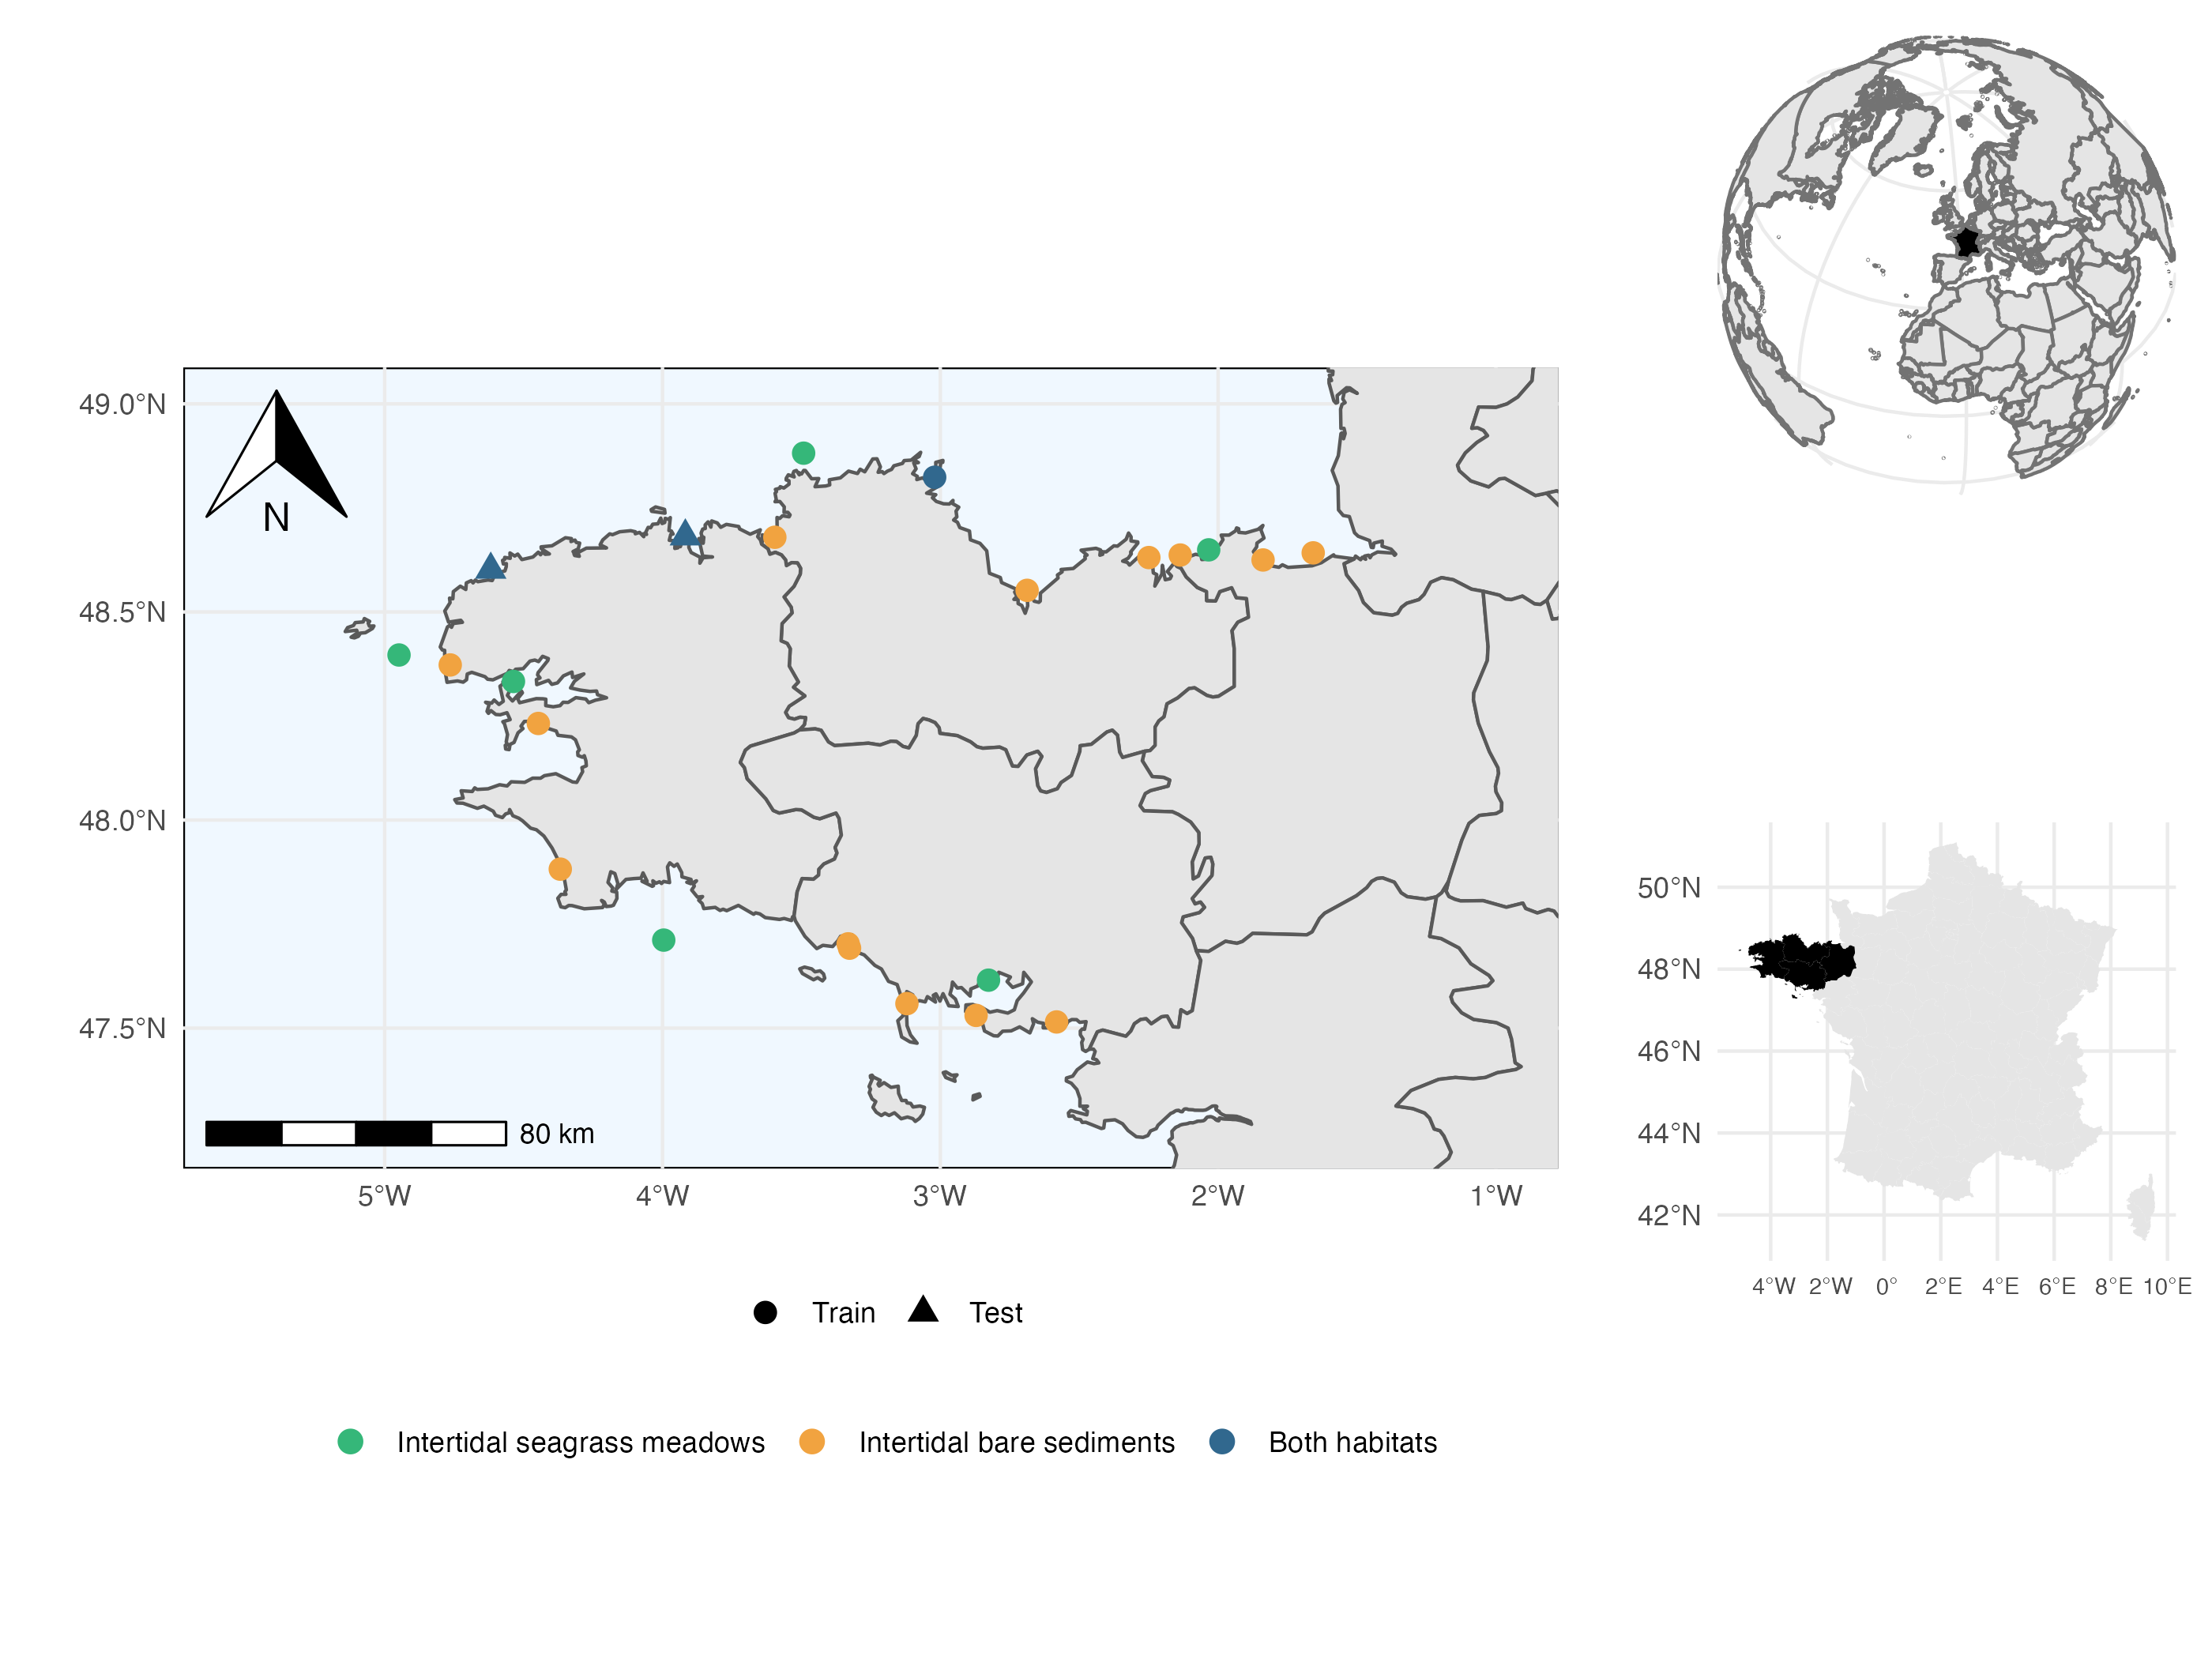
\includegraphics{03-Chapitre1/figures/supplementary/fig_supp1.png}
\caption{Map of the sampled sites. Point shapes vary according to their
contribution to model training set (circles ; used to evaluate model
explanatory power) as opposed to the two sites retained for independent
model testing (triangles ; used to evaluate model predictive power).
Point colours vary according to the presence or absence of the two
habitats in each site. The two test sites include the two habitats
(i.e.~seagrass and bare sand) and were chosen because they occur in
environmental conditions that can be considered average at the scale of
the region (thereby limiting extrapolation of the model) but still
harbour different communities, representative of the known diversity
gradient across the region.}\label{fig:chapt1supp1}
}
\end{figure}

\begin{figure}
\hypertarget{fig:chapt1supp2}{%
\centering
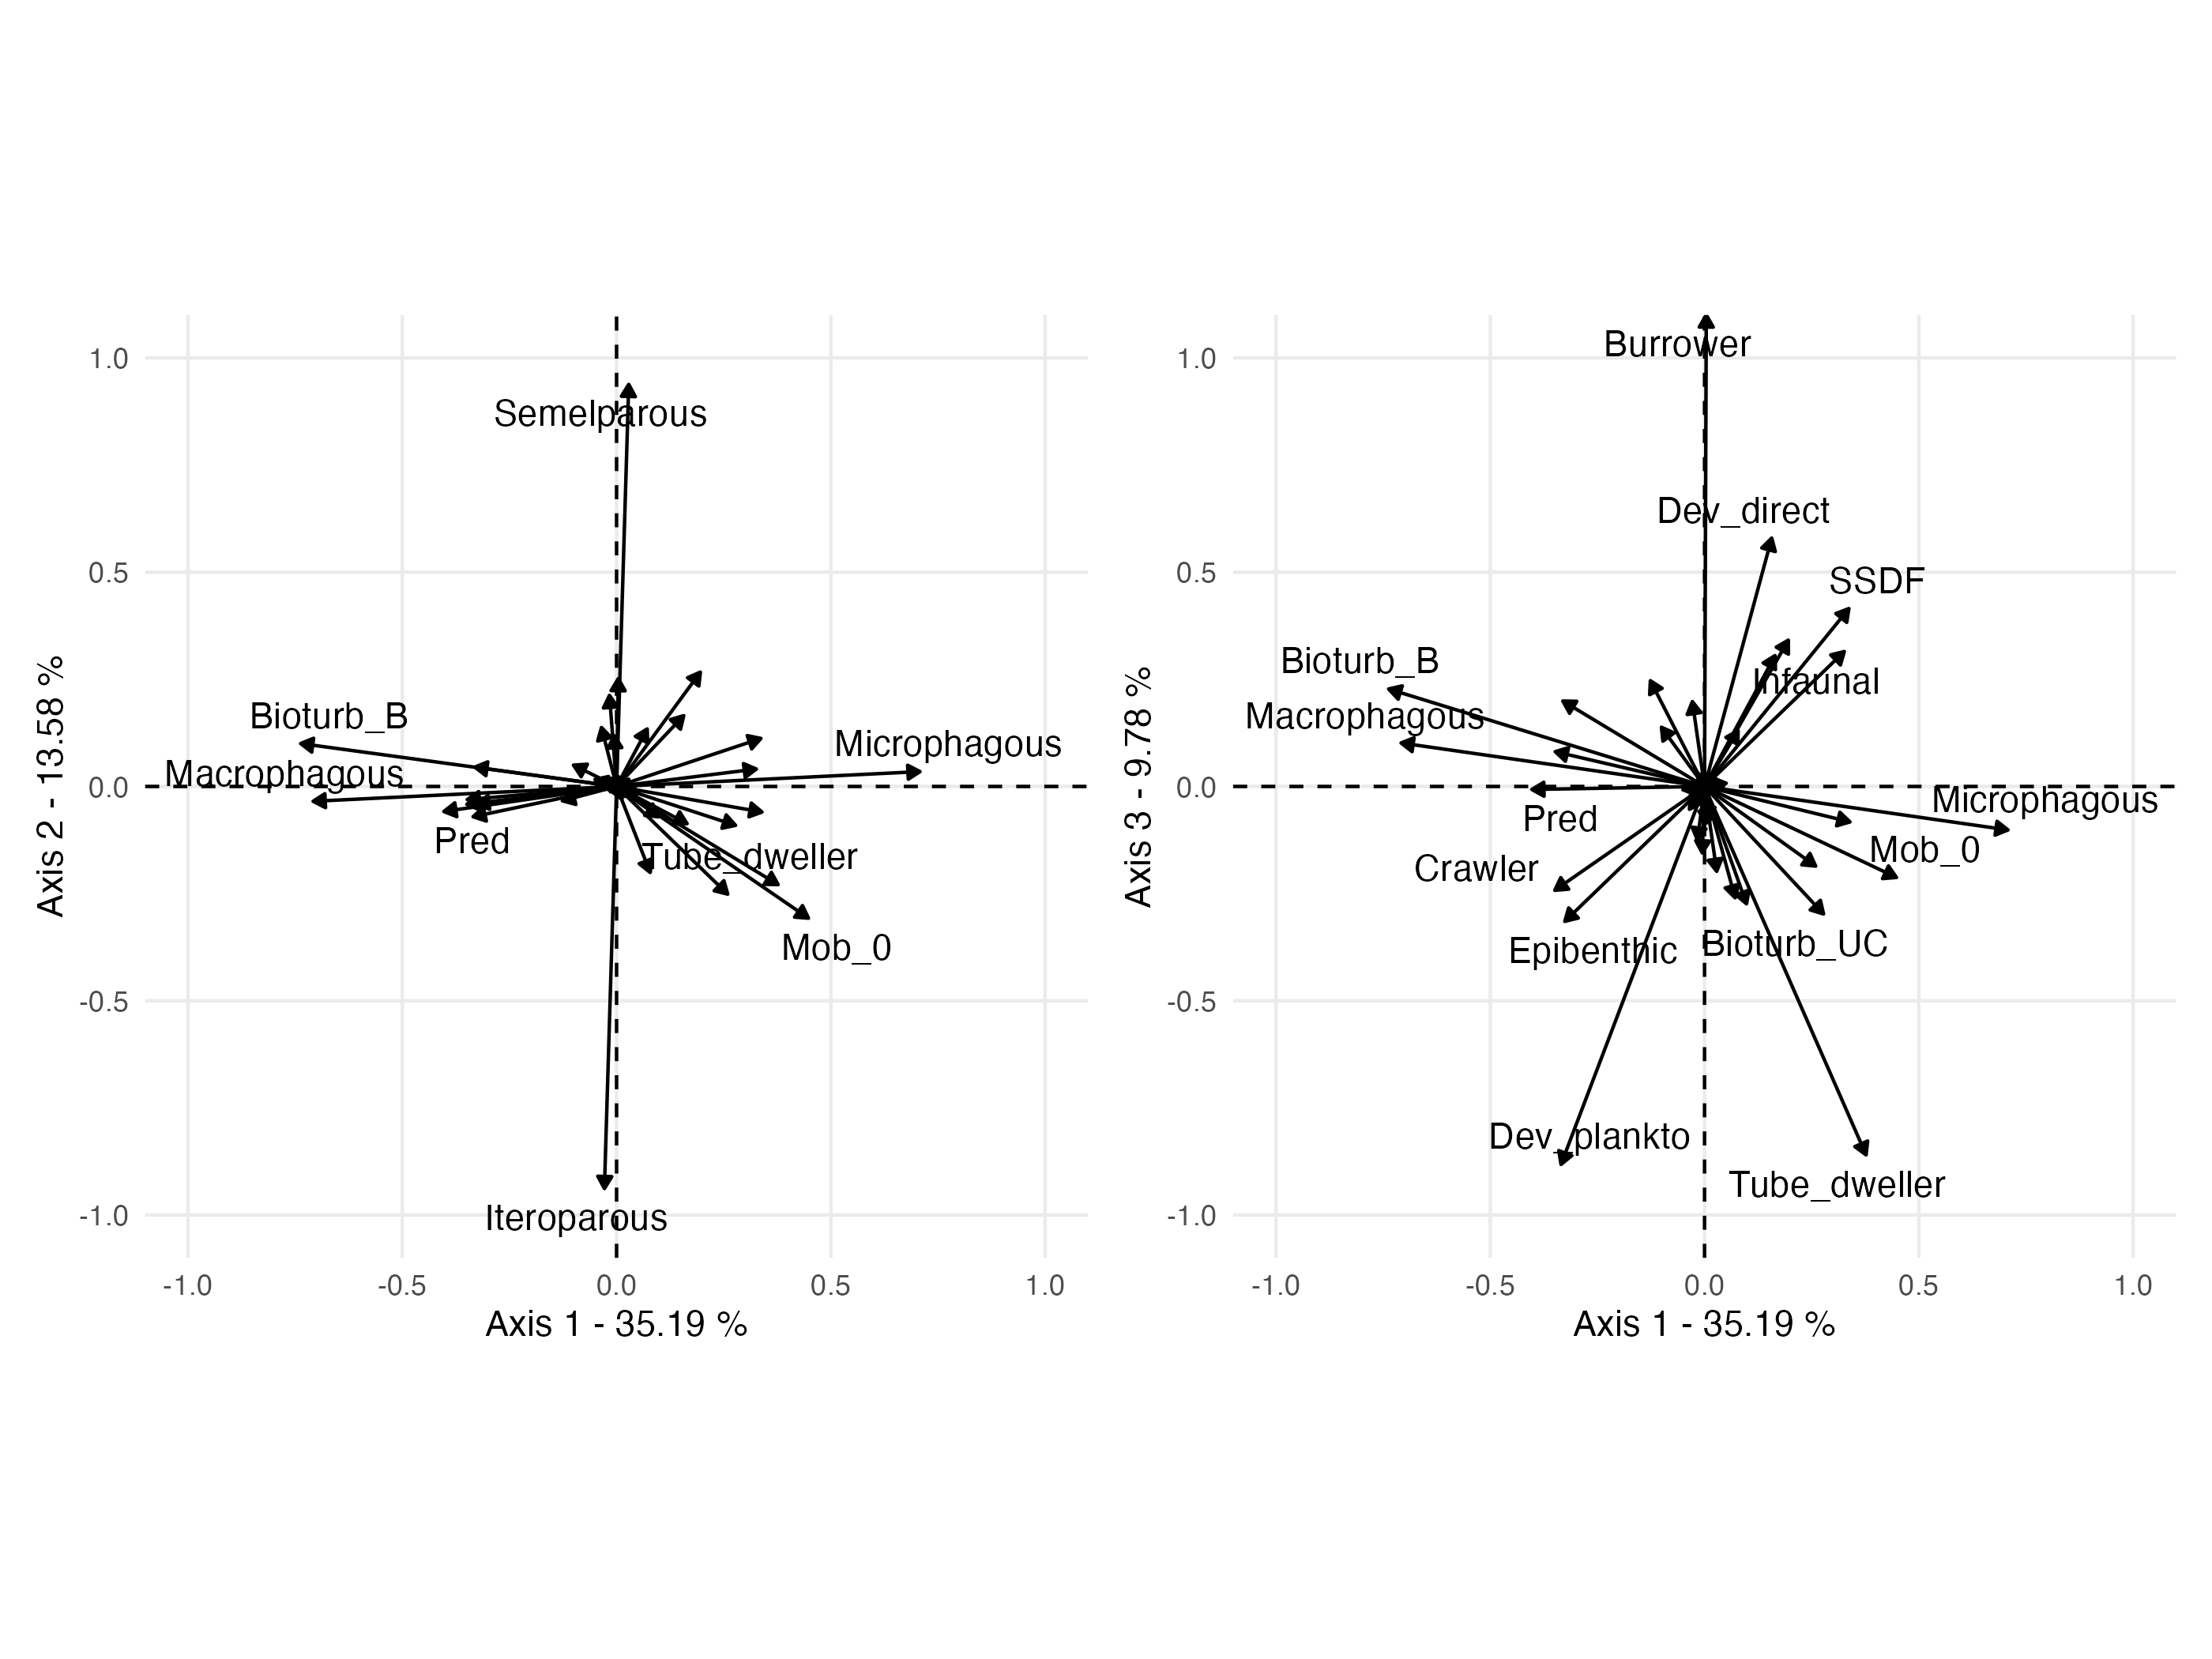
\includegraphics{03-Chapitre1/figures/supplementary/fig_supp2.png}
\caption{Fuzzy PCA of the species-by-trait matrix. The first three axes
represent 58.55\% of the total variance. The first axis distinguishes
sessile microphagous species (top positive values) from mobile
macrophagous predatory species (bottom negative values). The second axis
is a gradient of reproductive strategies (semelparous vs iteroparous).
The third axis distinguishes burrowers with direct development from
tube-dwellers with planktonic development. For abbreviations and meaning
of the trait modalities, see
\textcite{Boye_2019a}.}\label{fig:chapt1supp2}
}
\end{figure}

\begin{figure}
\hypertarget{fig:chapt1supp3}{%
\centering
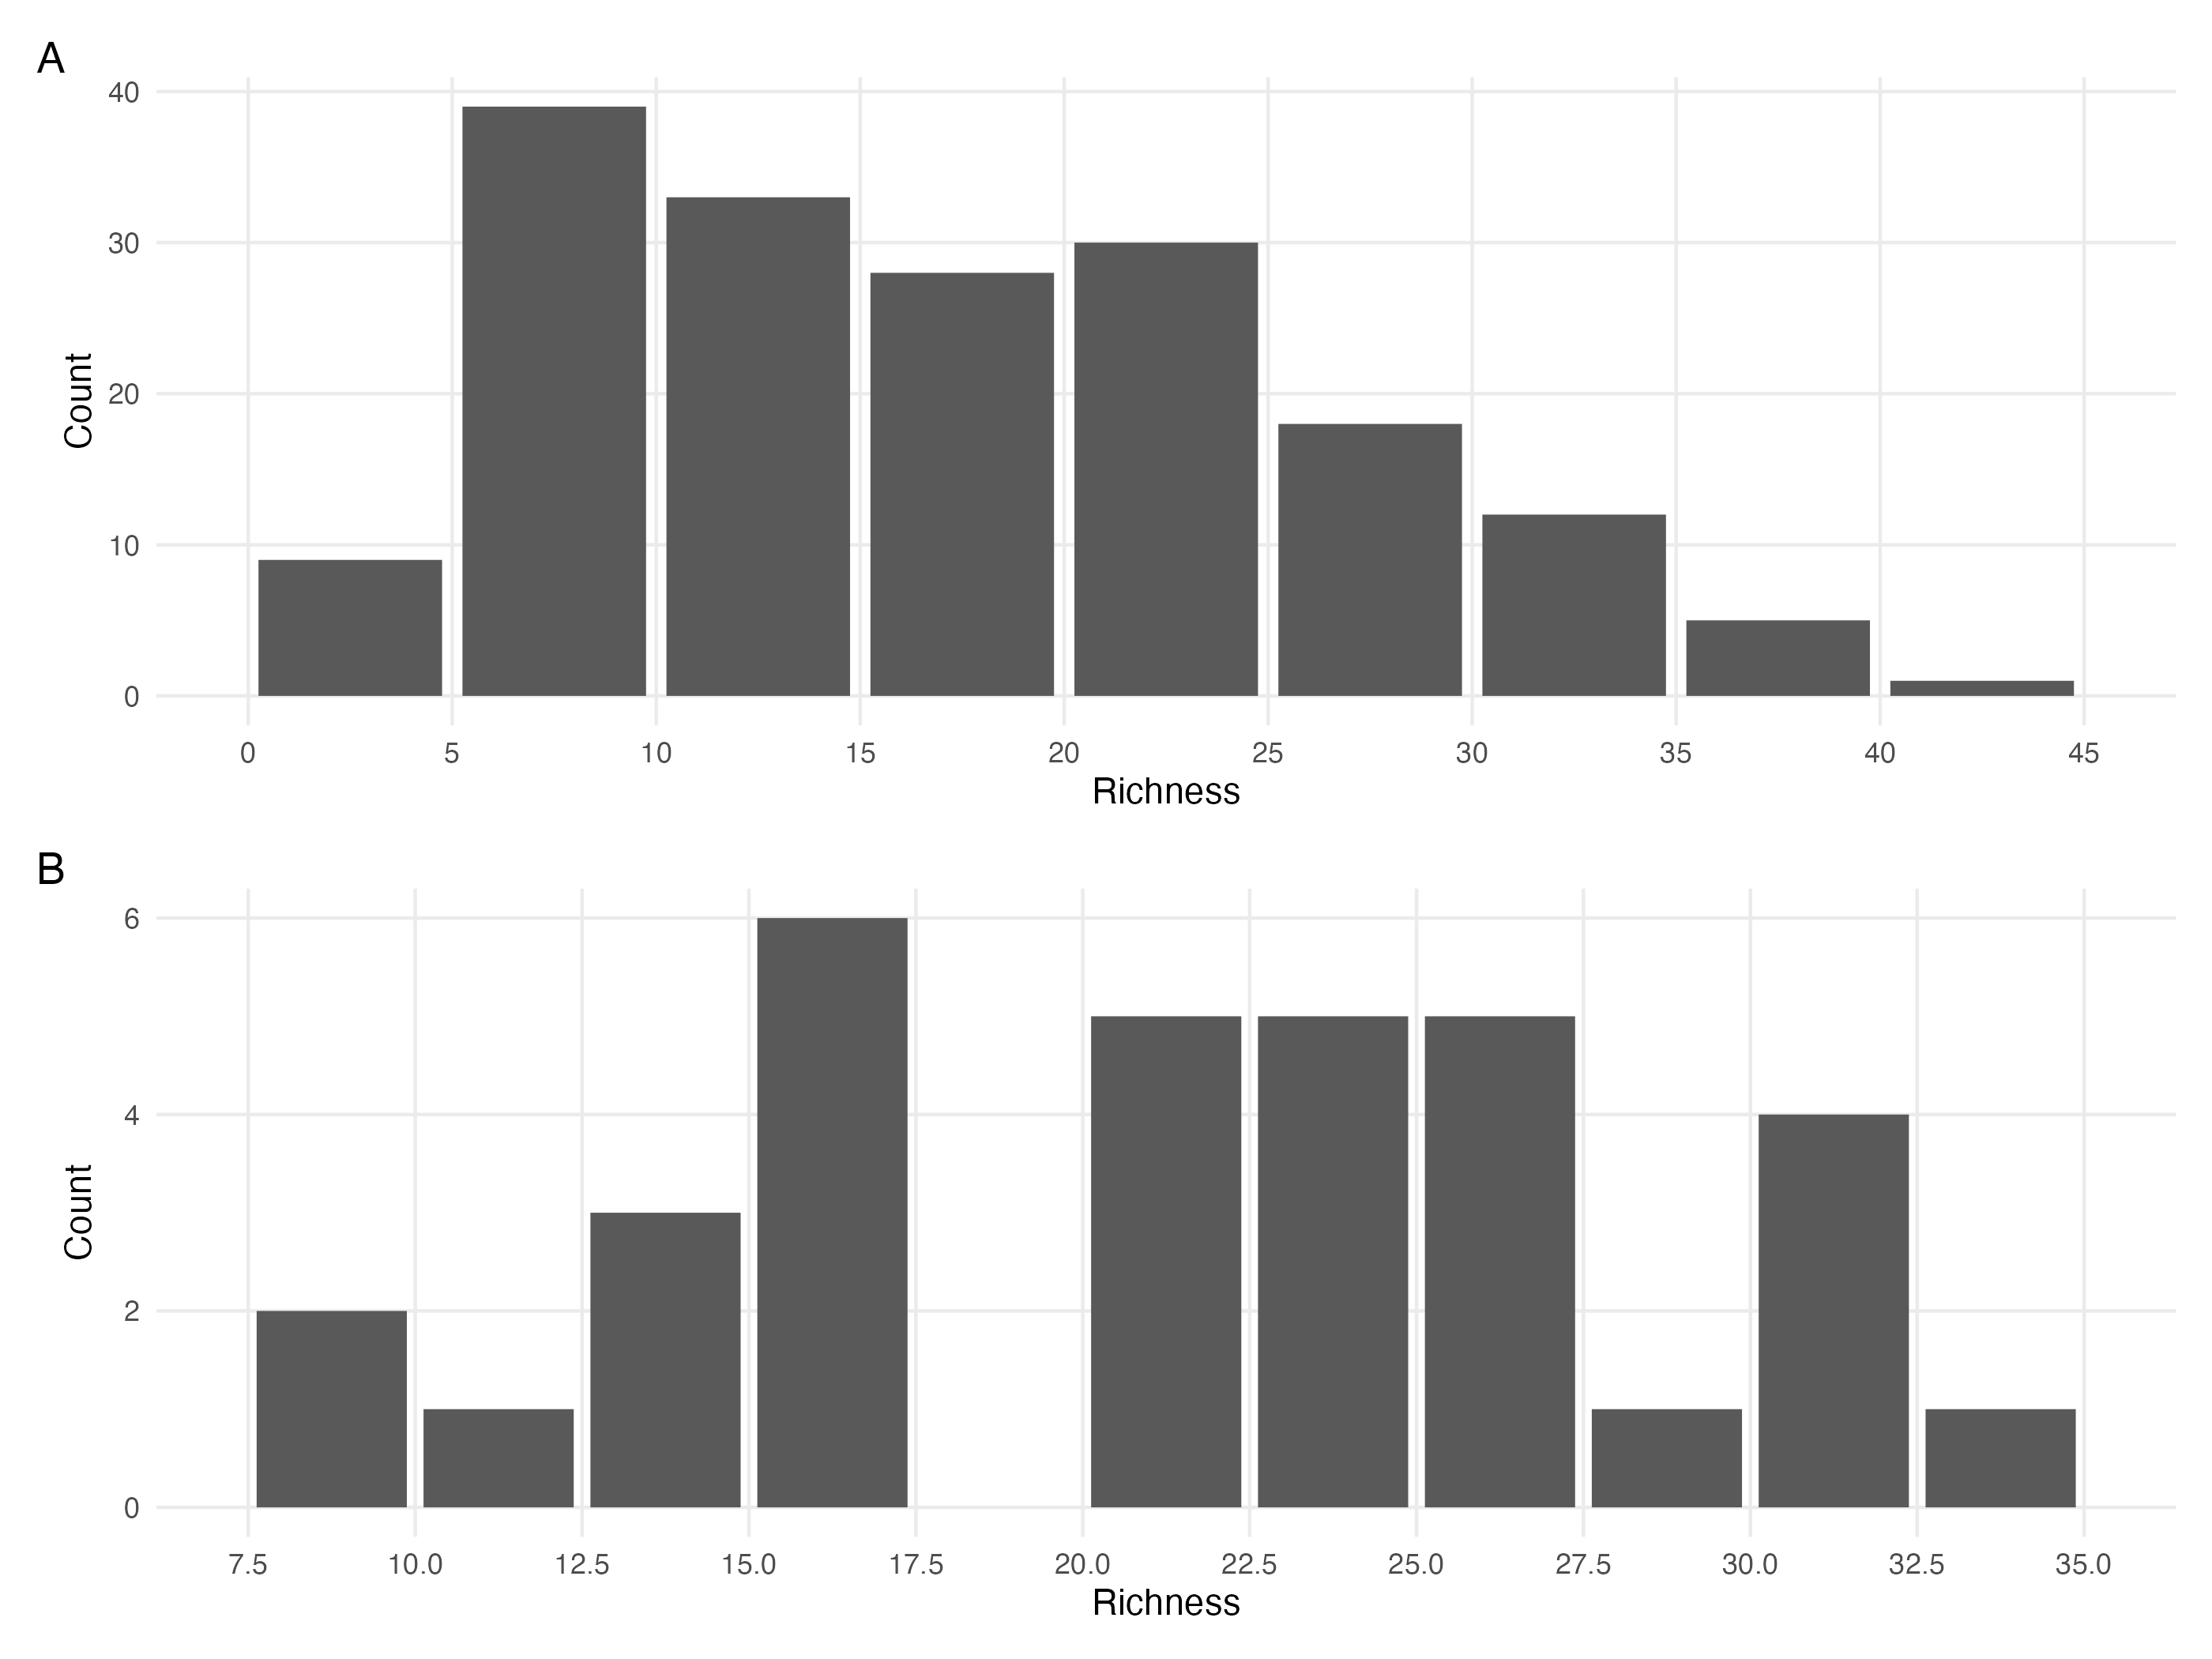
\includegraphics{03-Chapitre1/figures/supplementary/fig_supp3.png}
\caption{A. Distribution of the number of species in the samples (site
times habitat times year) of the train dataset. B. Distribution of the
number of species in the samples (site times habitat times year) of the
test dataset.}\label{fig:chapt1supp3}
}
\end{figure}

\begin{figure}
\hypertarget{fig:chapt1supp4}{%
\centering
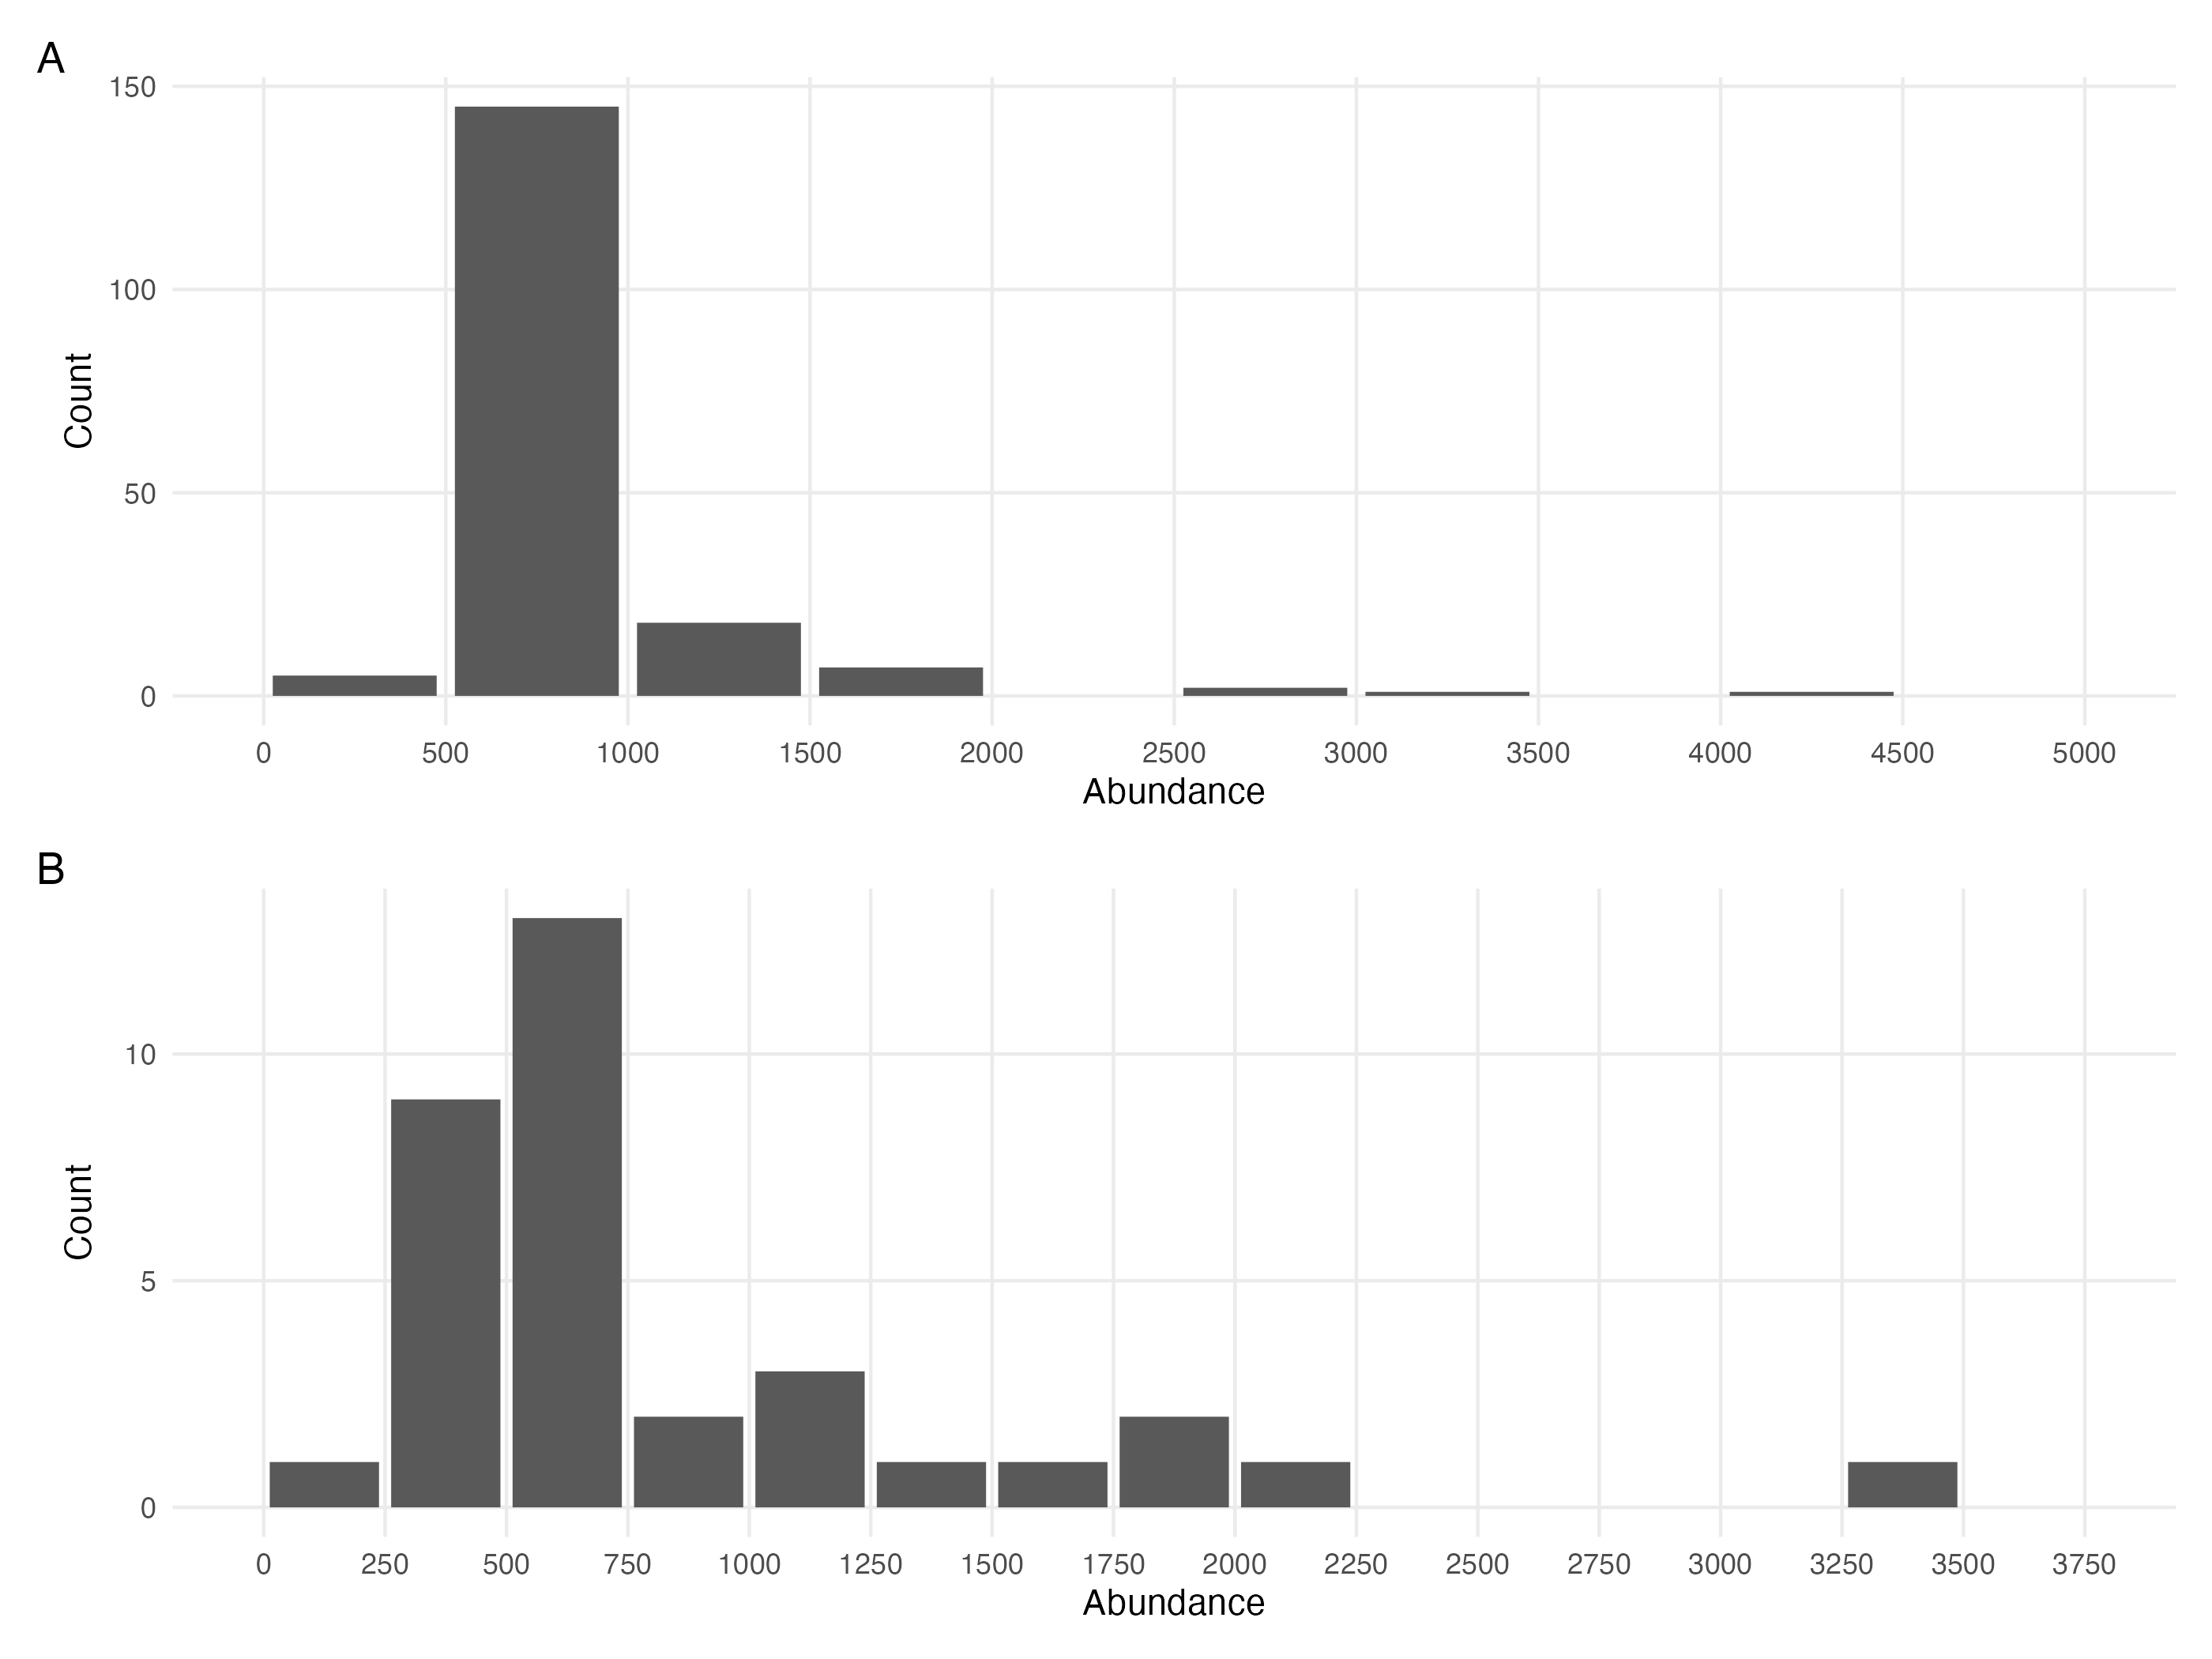
\includegraphics{03-Chapitre1/figures/supplementary/fig_supp4.png}
\caption{A. Distribution of the total number of individuals (abundance)
in the samples (site times habitat times year) of the train dataset. B.
Distribution of the total number of individuals (abundance) in the
samples (site times habitat times year) of the test
dataset.}\label{fig:chapt1supp4}
}
\end{figure}

\hypertarget{environmental-data-acquisition}{%
\subsection*{Environmental data
acquisition}\label{environmental-data-acquisition}}

The models used in this study incorporate a dataset consisting of seven
environmental variables related to oceanography, hydrography, and
granulometry obtained from \textcite{Boye_2019b} The oceanographic
variables include the standard deviation of salinity, surface water
temperature, mean velocity of currents, and fetch, which were obtained
from the PREVIMER database \autocite{Lecornu_2009} based on the MARS3D
model \autocite{Lazure_2008}. The variables were averaged by extracting
daily data for the sampled year at the site coordinates and the eight
adjacent cells. The fetch was calculated as the average length of nine
radiating fetch segments with a maximum distance of 300km. The
granulometry variables were derived from sediment cores that were taken
along with associated fauna. The cores were dried, separated into 15
fractions, and the Trask index was calculated as the ratio of the 25th
to 75th percentile of the grain distribution. Organic matter mass was
estimated through the loss of mass after combustion in an oven.

\clearpage

\hypertarget{appendixB-chapter1}{%
\section*{Appendix B - Model Convergence}\label{appendixB-chapter1}}
\addcontentsline{toc}{section}{Appendix B - Model Convergence}

\hypertarget{environmental-coefficients}{%
\subsection*{Environmental
coefficients}\label{environmental-coefficients}}

\hypertarget{tbl:chapt1beta_convergence}{}
\begin{longtable}[]{@{}
  >{\centering\arraybackslash}p{(\columnwidth - 8\tabcolsep) * \real{0.1905}}
  >{\raggedright\arraybackslash}p{(\columnwidth - 8\tabcolsep) * \real{0.1714}}
  >{\centering\arraybackslash}p{(\columnwidth - 8\tabcolsep) * \real{0.2286}}
  >{\raggedleft\arraybackslash}p{(\columnwidth - 8\tabcolsep) * \real{0.2095}}
  >{\raggedleft\arraybackslash}p{(\columnwidth - 8\tabcolsep) * \real{0.2000}}@{}}
\caption{\label{tbl:chapt1beta_convergence}Potential scale reduction
factors (PSRF) and effective sample sizes (ESS) for environmental
regression parameters (i.e beta coefficients) estimated estimated for
the four different models (Bench, Ph, TrPh, WhC) fitted either to
abundance or presence-absence data. For further details see Fig. S5 to
Fig. S12.}\tabularnewline
\toprule\noalign{}
\begin{minipage}[b]{\linewidth}\centering
Model
\end{minipage} & \begin{minipage}[b]{\linewidth}\raggedright
Data Type
\end{minipage} & \begin{minipage}[b]{\linewidth}\centering
Number of coefficients
\end{minipage} & \begin{minipage}[b]{\linewidth}\raggedleft
PSRF (mean \(\pm\) sd)
\end{minipage} & \begin{minipage}[b]{\linewidth}\raggedleft
ESS (mean \(\pm\) sd)
\end{minipage} \\
\midrule\noalign{}
\endfirsthead
\toprule\noalign{}
\begin{minipage}[b]{\linewidth}\centering
Model
\end{minipage} & \begin{minipage}[b]{\linewidth}\raggedright
Data Type
\end{minipage} & \begin{minipage}[b]{\linewidth}\centering
Number of coefficients
\end{minipage} & \begin{minipage}[b]{\linewidth}\raggedleft
PSRF (mean \(\pm\) sd)
\end{minipage} & \begin{minipage}[b]{\linewidth}\raggedleft
ESS (mean \(\pm\) sd)
\end{minipage} \\
\midrule\noalign{}
\endhead
\bottomrule\noalign{}
\endlastfoot
Benchmark & Abundance & 1485 & 1.18 \(\pm\) 0.267 & 701 \(\pm\) 576 \\
Benchmark & Presence/Absence & 1485 & 1.00 \(\pm\) 0.002 & 4967 \(\pm\)
417 \\
Phylogeny & Abundance & 1485 & 1.18 \(\pm\) 0.204 & 566 \(\pm\) 420 \\
Phylogeny & Presence/Absence & 1485 & 1.00 \(\pm\) 0.001 & 4947 \(\pm\)
408 \\
Traits \& Phylogeny & Abundance & 1485 & 1.21 \(\pm\) 0.317 & 489
\(\pm\) 358 \\
Traits \& Phylogeny & Presence/Absence & 1485 & 1.00 \(\pm\) 0.008 &
11459 \(\pm\) 2649 \\
Whole Community & Abundance & 4170 & 1.21 \(\pm\) 0.287 & 739 \(\pm\)
631 \\
Whole Community & Presence/Absence & 4170 & 1.00 \(\pm\) 0.002 & 4962
\(\pm\) 406 \\
\end{longtable}

\begin{figure}
\hypertarget{fig:chapt1bench_ab_beta}{%
\centering
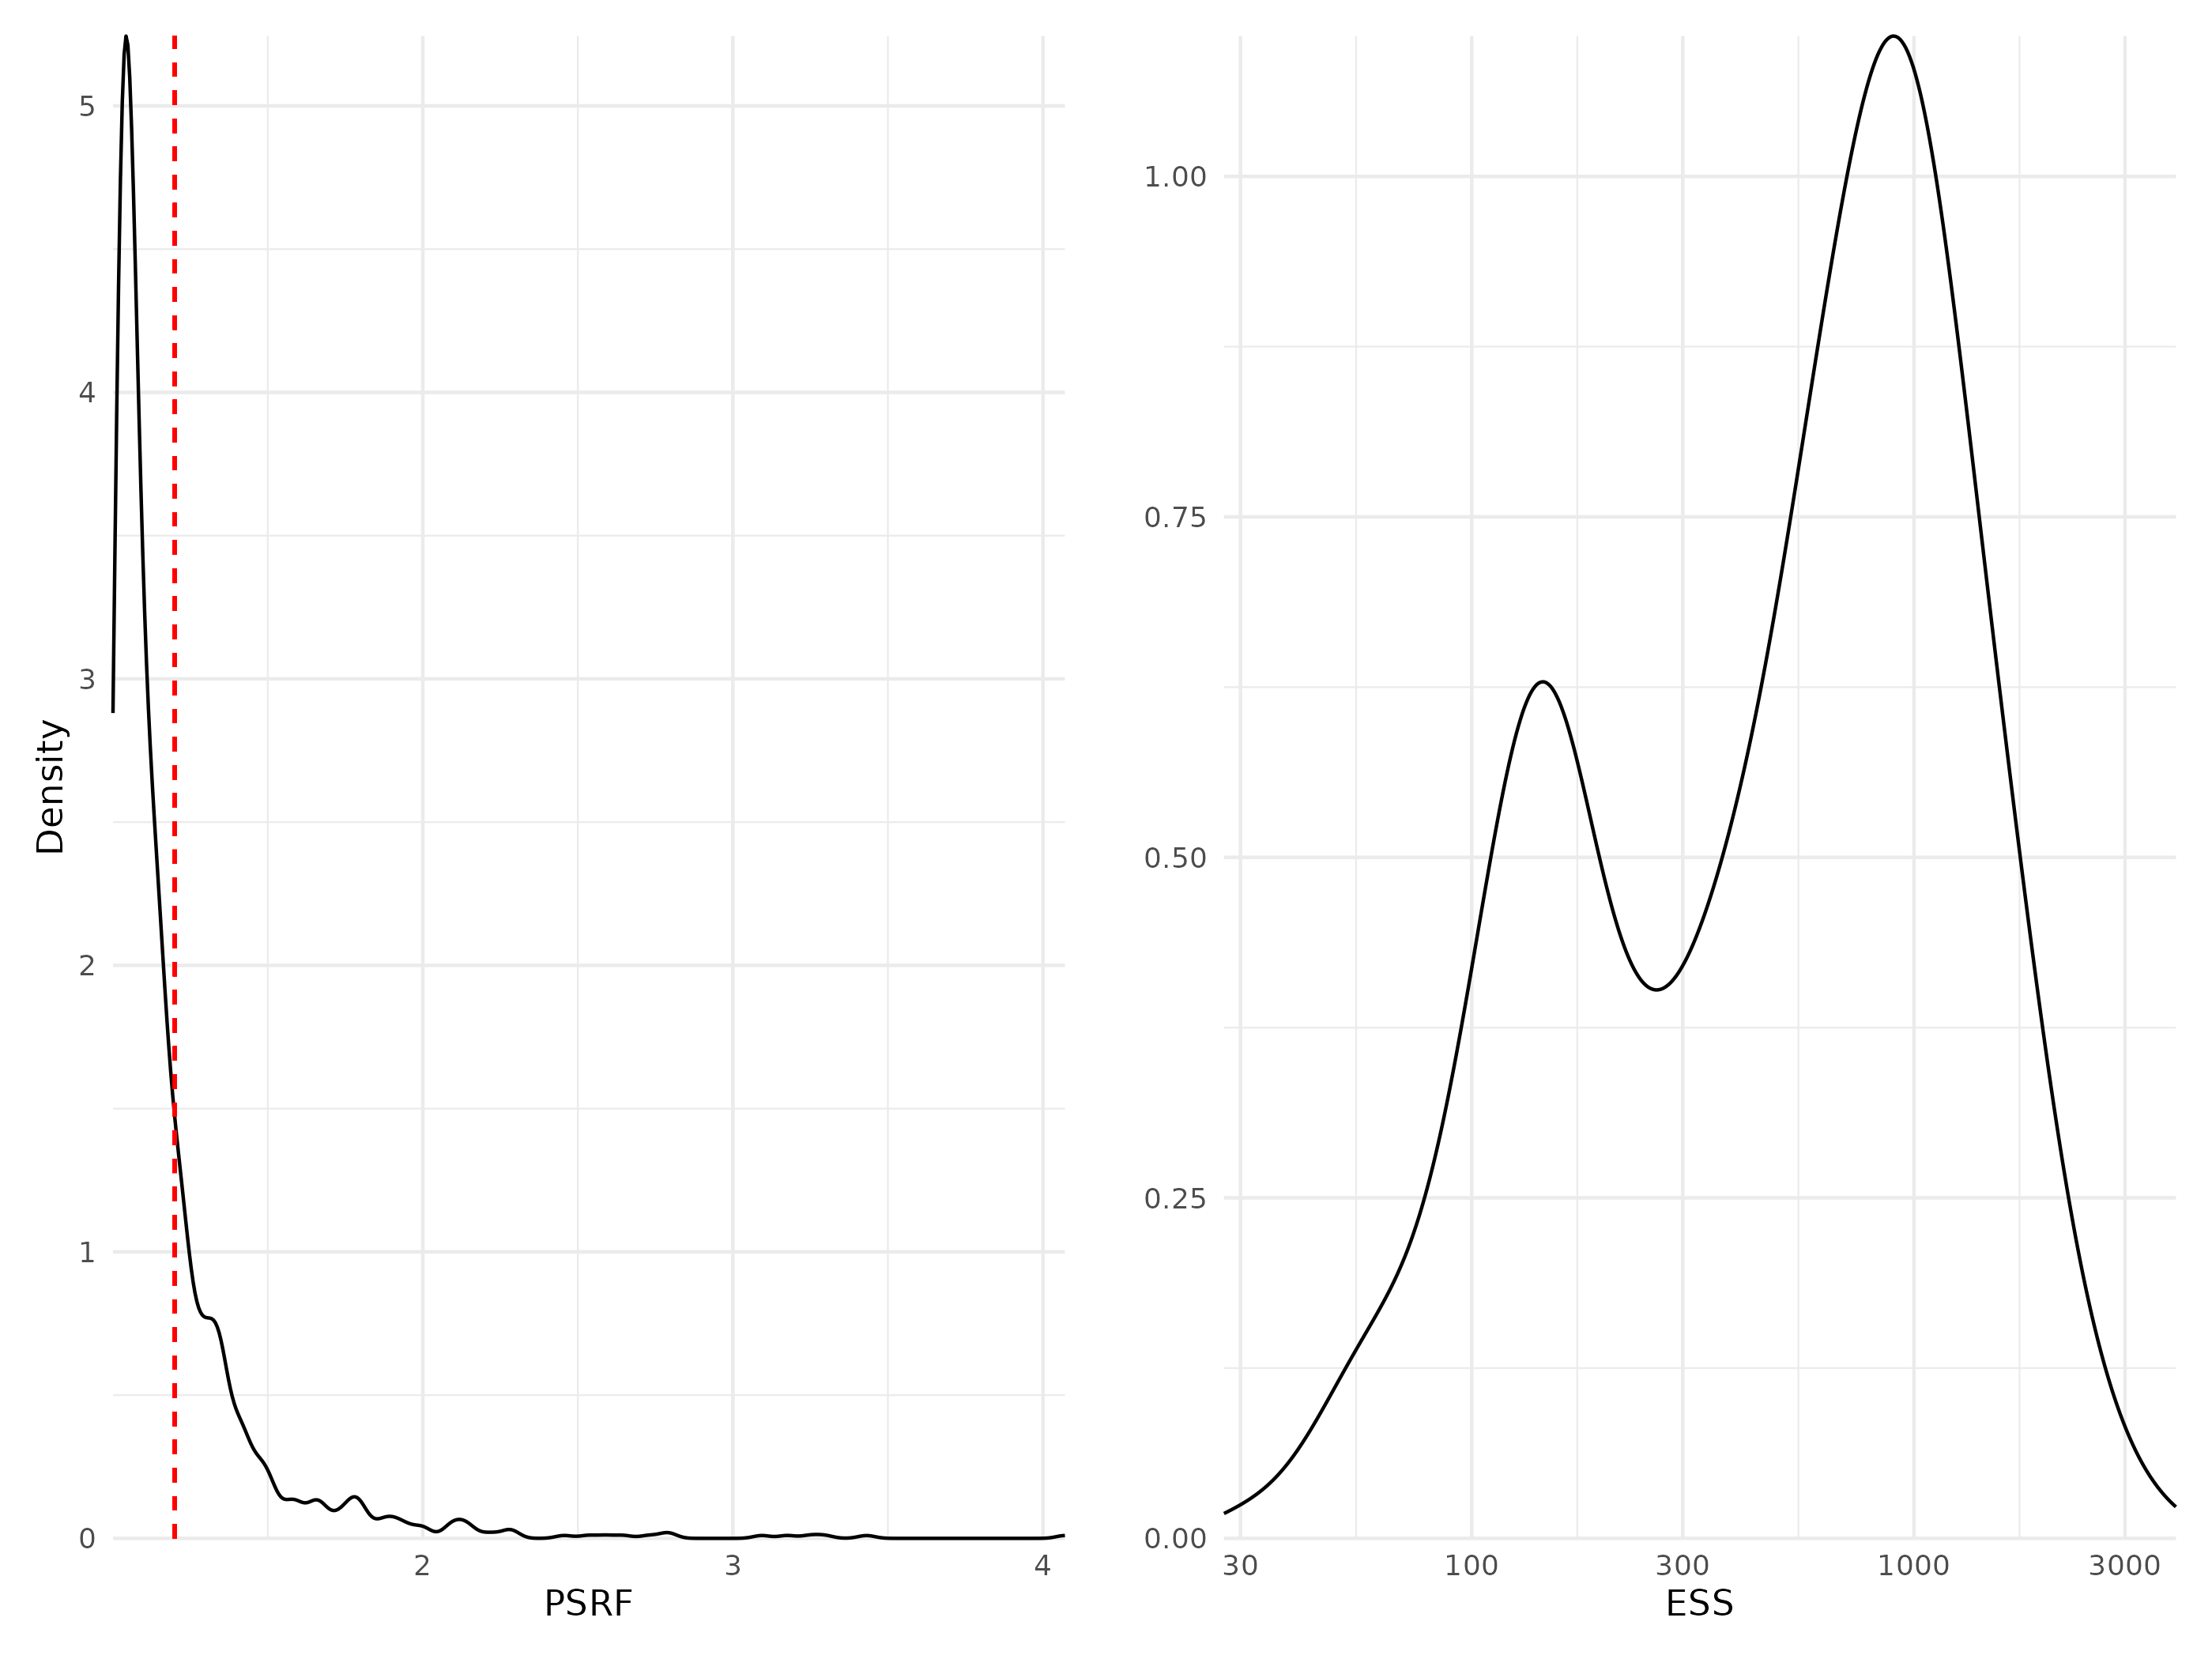
\includegraphics{03-Chapitre1/figures/supplementary/fig_supp_conv_beta_PolychaetaAB.png}
\caption{Density curves of potential scale reduction factors (PSRF see
\textcite{Brooks_1998}; left panel) and effective sample sizes (ESS;
right panel) for Beta regression parameters (i.e environmental
coefficients) estimated for the benchmark model fitted with abundance
data. For PSRF, values greater than 1.2 (dotted red line) indicate
potential convergence issues. ESS estimates the number of independent
samples used to estimate each parameter (the more the
better).}\label{fig:chapt1bench_ab_beta}
}
\end{figure}

\begin{figure}
\hypertarget{fig:chapt1bench_pa_beta}{%
\centering
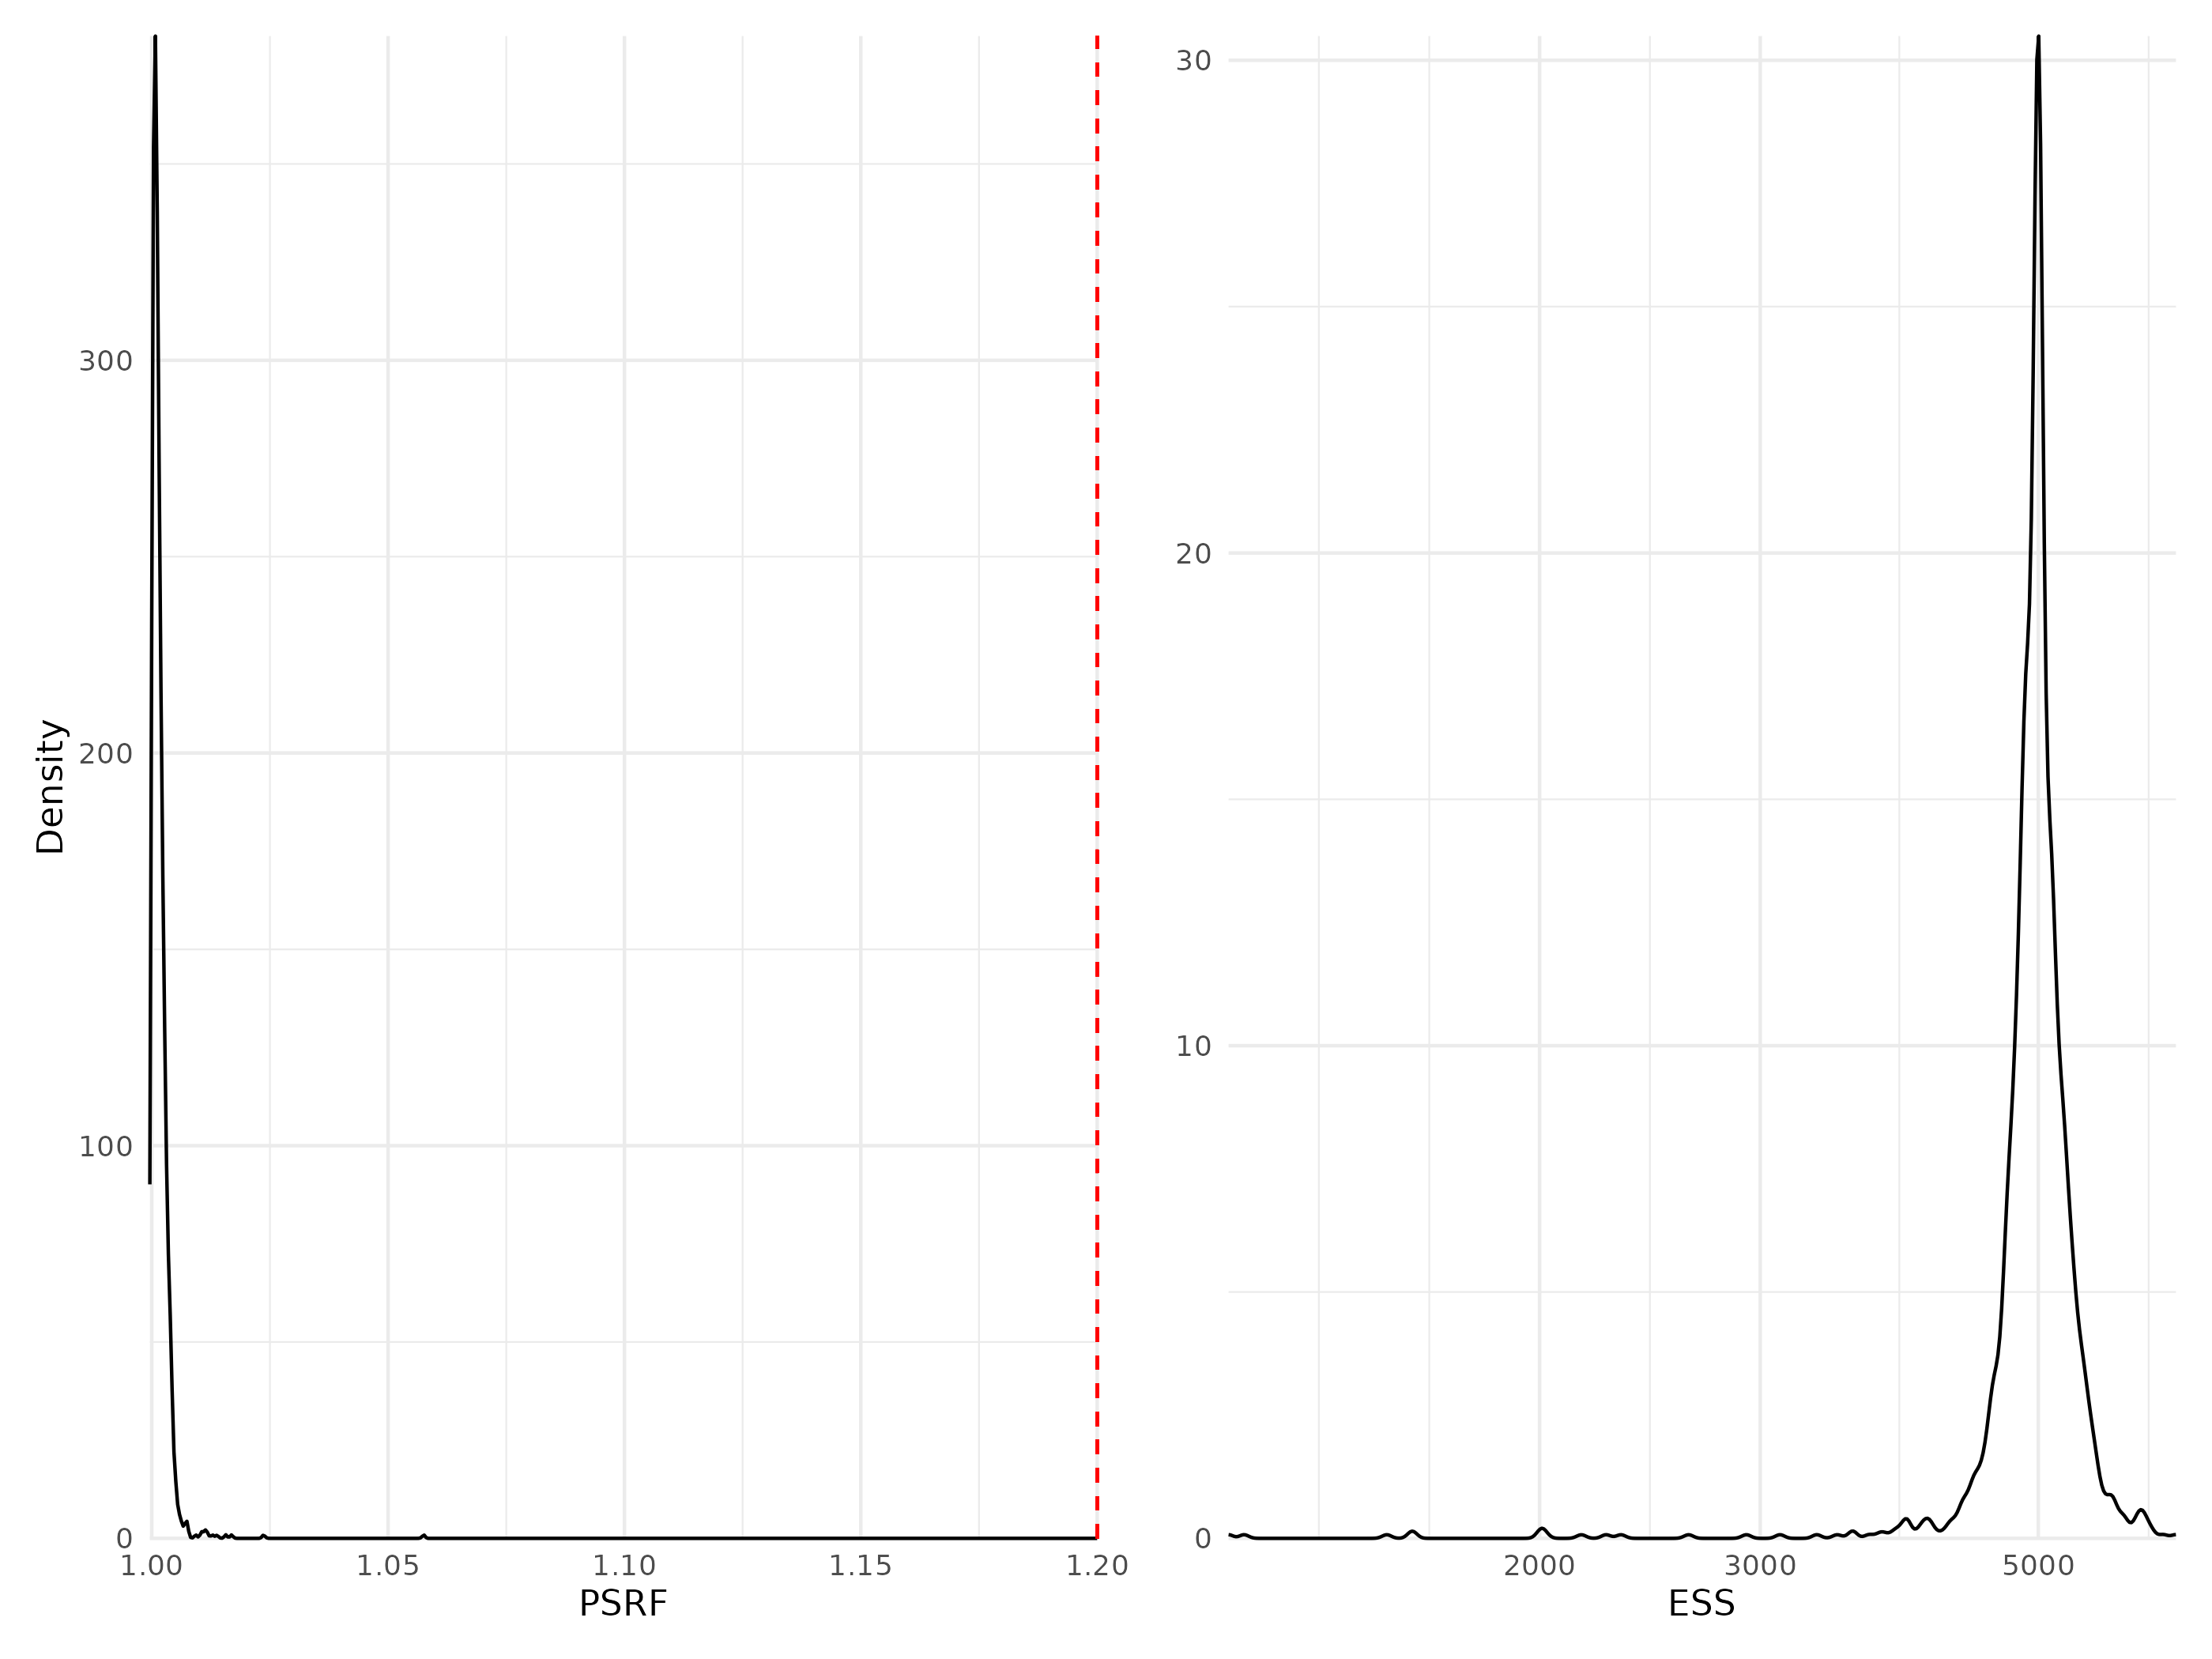
\includegraphics{03-Chapitre1/figures/supplementary/fig_supp_conv_beta_PolychaetaPA.png}
\caption{Density curves of potential scale reduction factors (PSRF see
\textcite{Brooks_1998}; left panel) and effective sample sizes (ESS;
right panel) for Beta regression parameters (i.e environmental
coefficients) estimated for the benchmark model fitted with
presence/absence data. For further details see Fig.
S5.}\label{fig:chapt1bench_pa_beta}
}
\end{figure}

\begin{figure}
\hypertarget{fig:chapt1phylo_ab_beta}{%
\centering
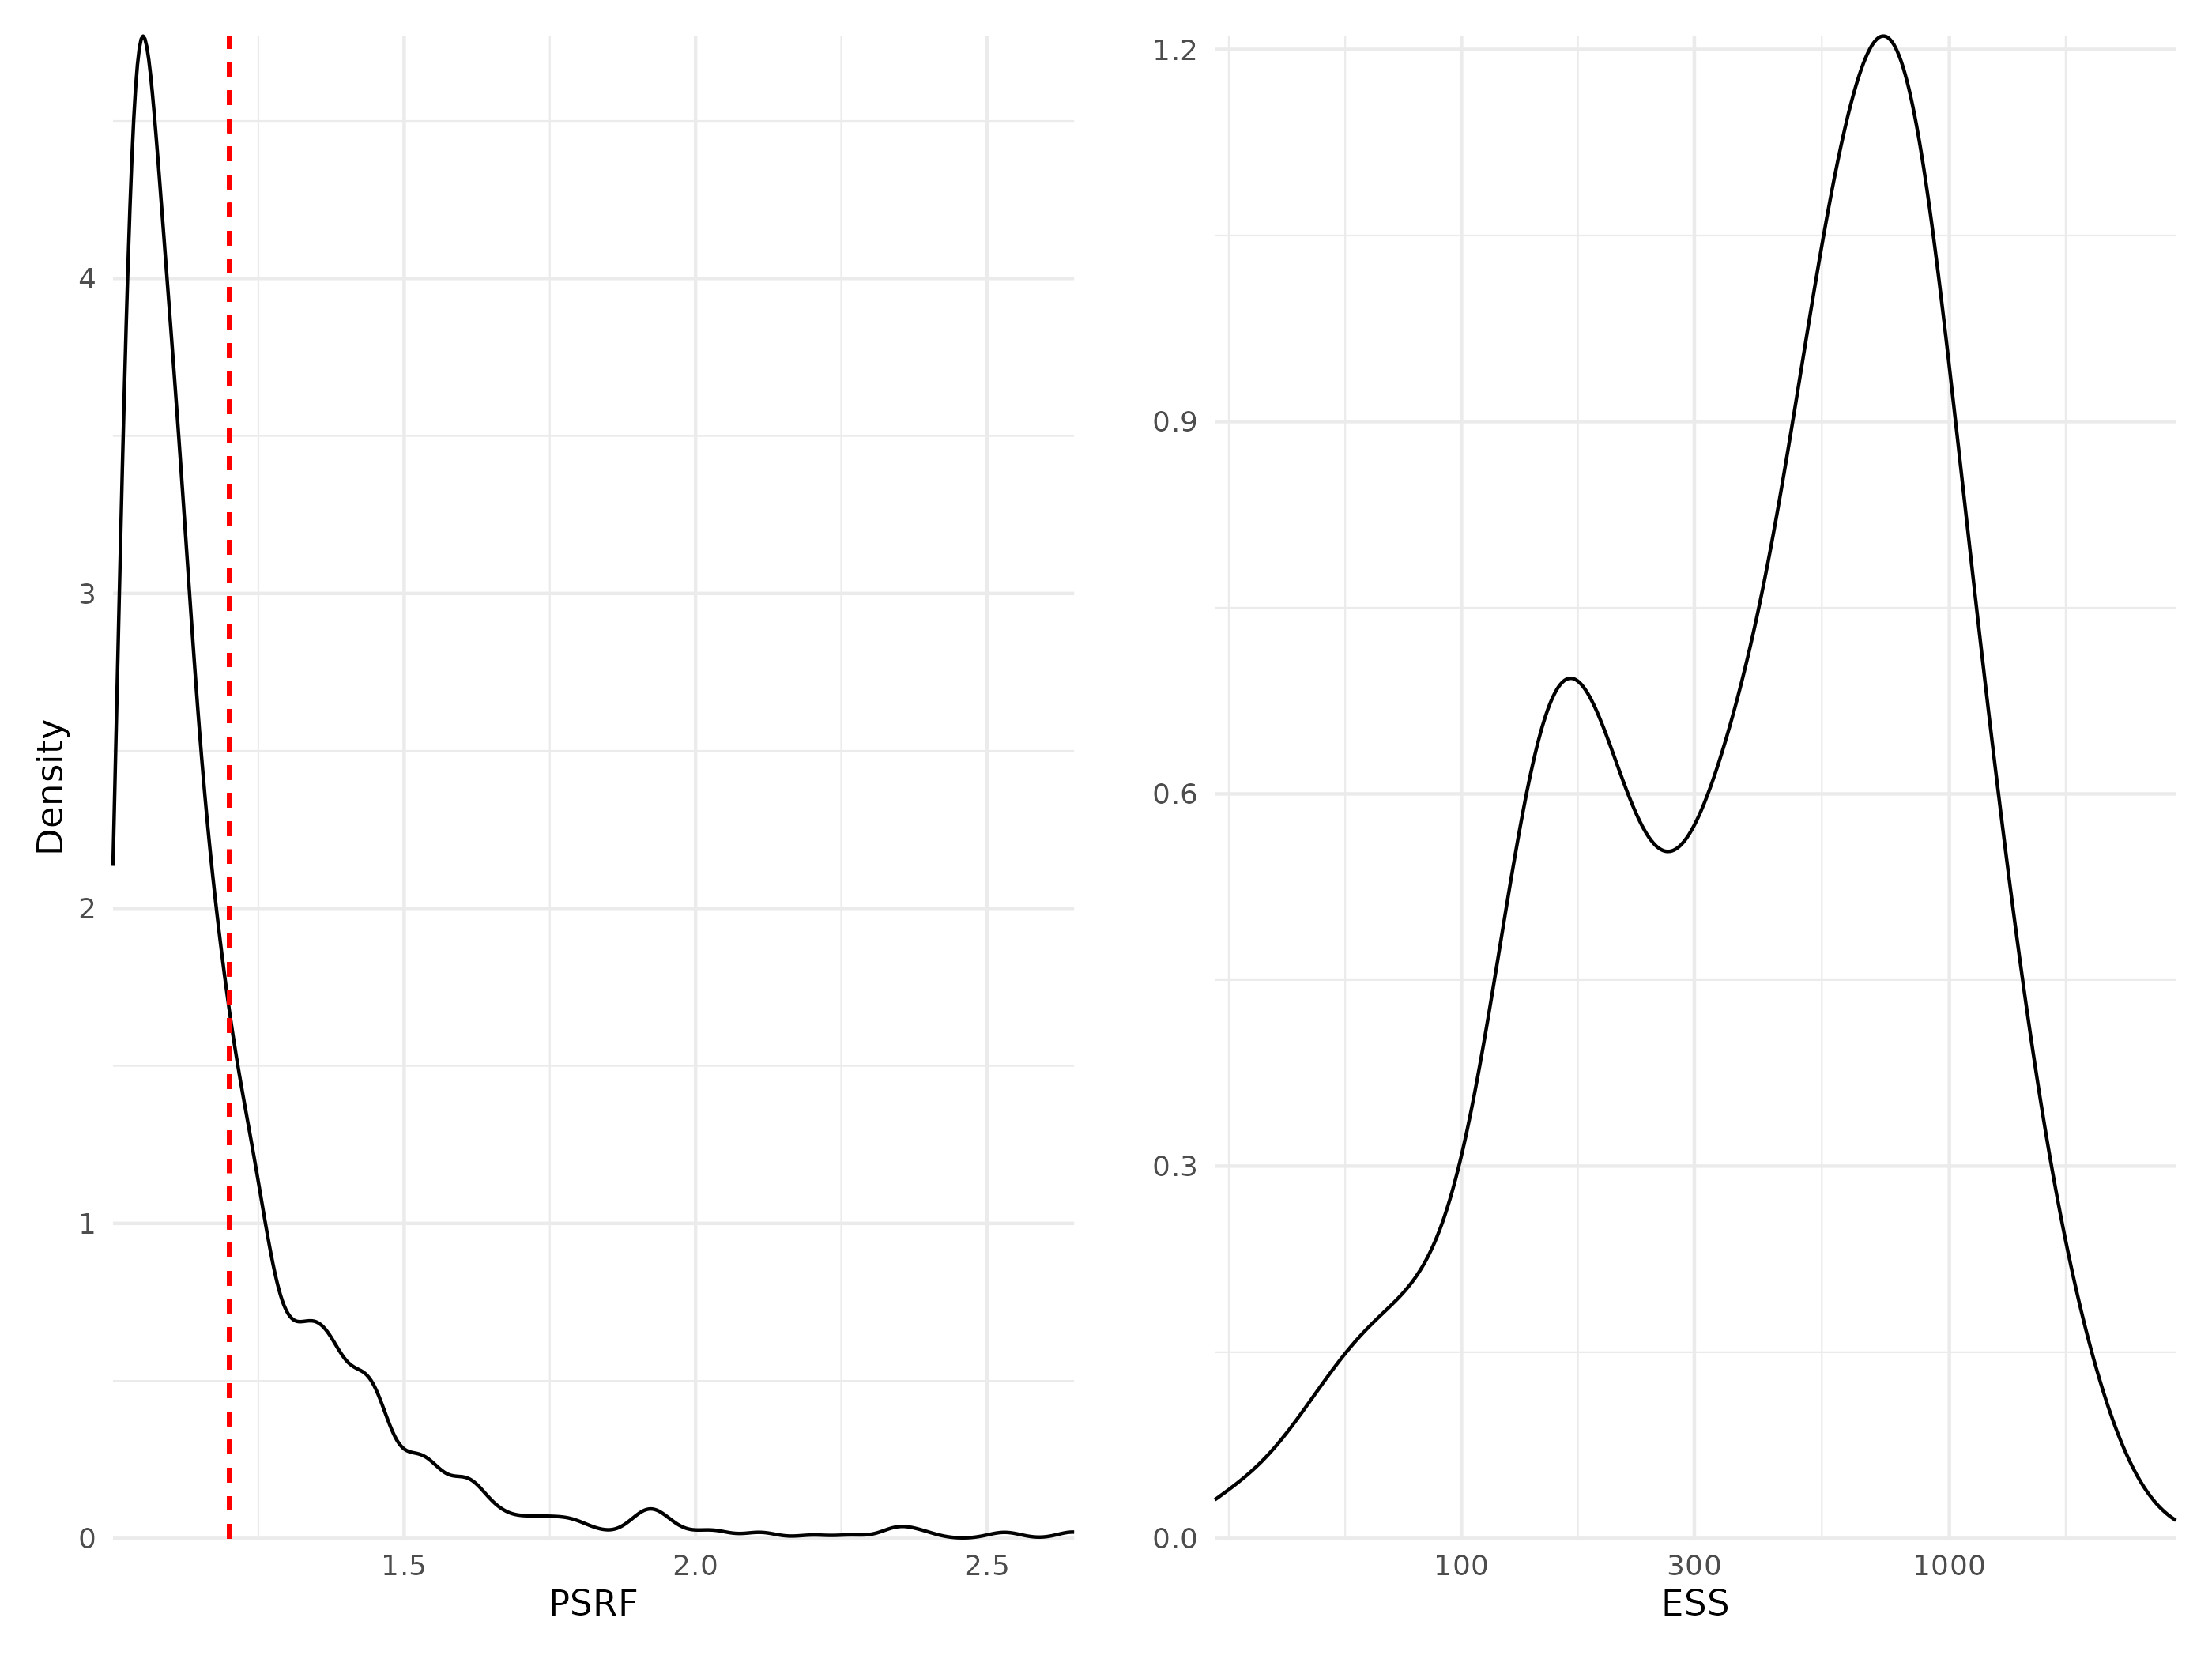
\includegraphics{03-Chapitre1/figures/supplementary/fig_supp_conv_beta_PolychaetaPhylogenyAB.png}
\caption{Density curves of potential scale reduction factors (PSRF see
\textcite{Brooks_1998}; left panel) and effective sample sizes (ESS;
right panel) for Beta regression parameters (i.e environmental
coefficients) estimated for the phylogeny model fitted with abundance
data. For further details see Fig. S5.}\label{fig:chapt1phylo_ab_beta}
}
\end{figure}

\begin{figure}
\hypertarget{fig:chapt1phylo_pa_beta}{%
\centering
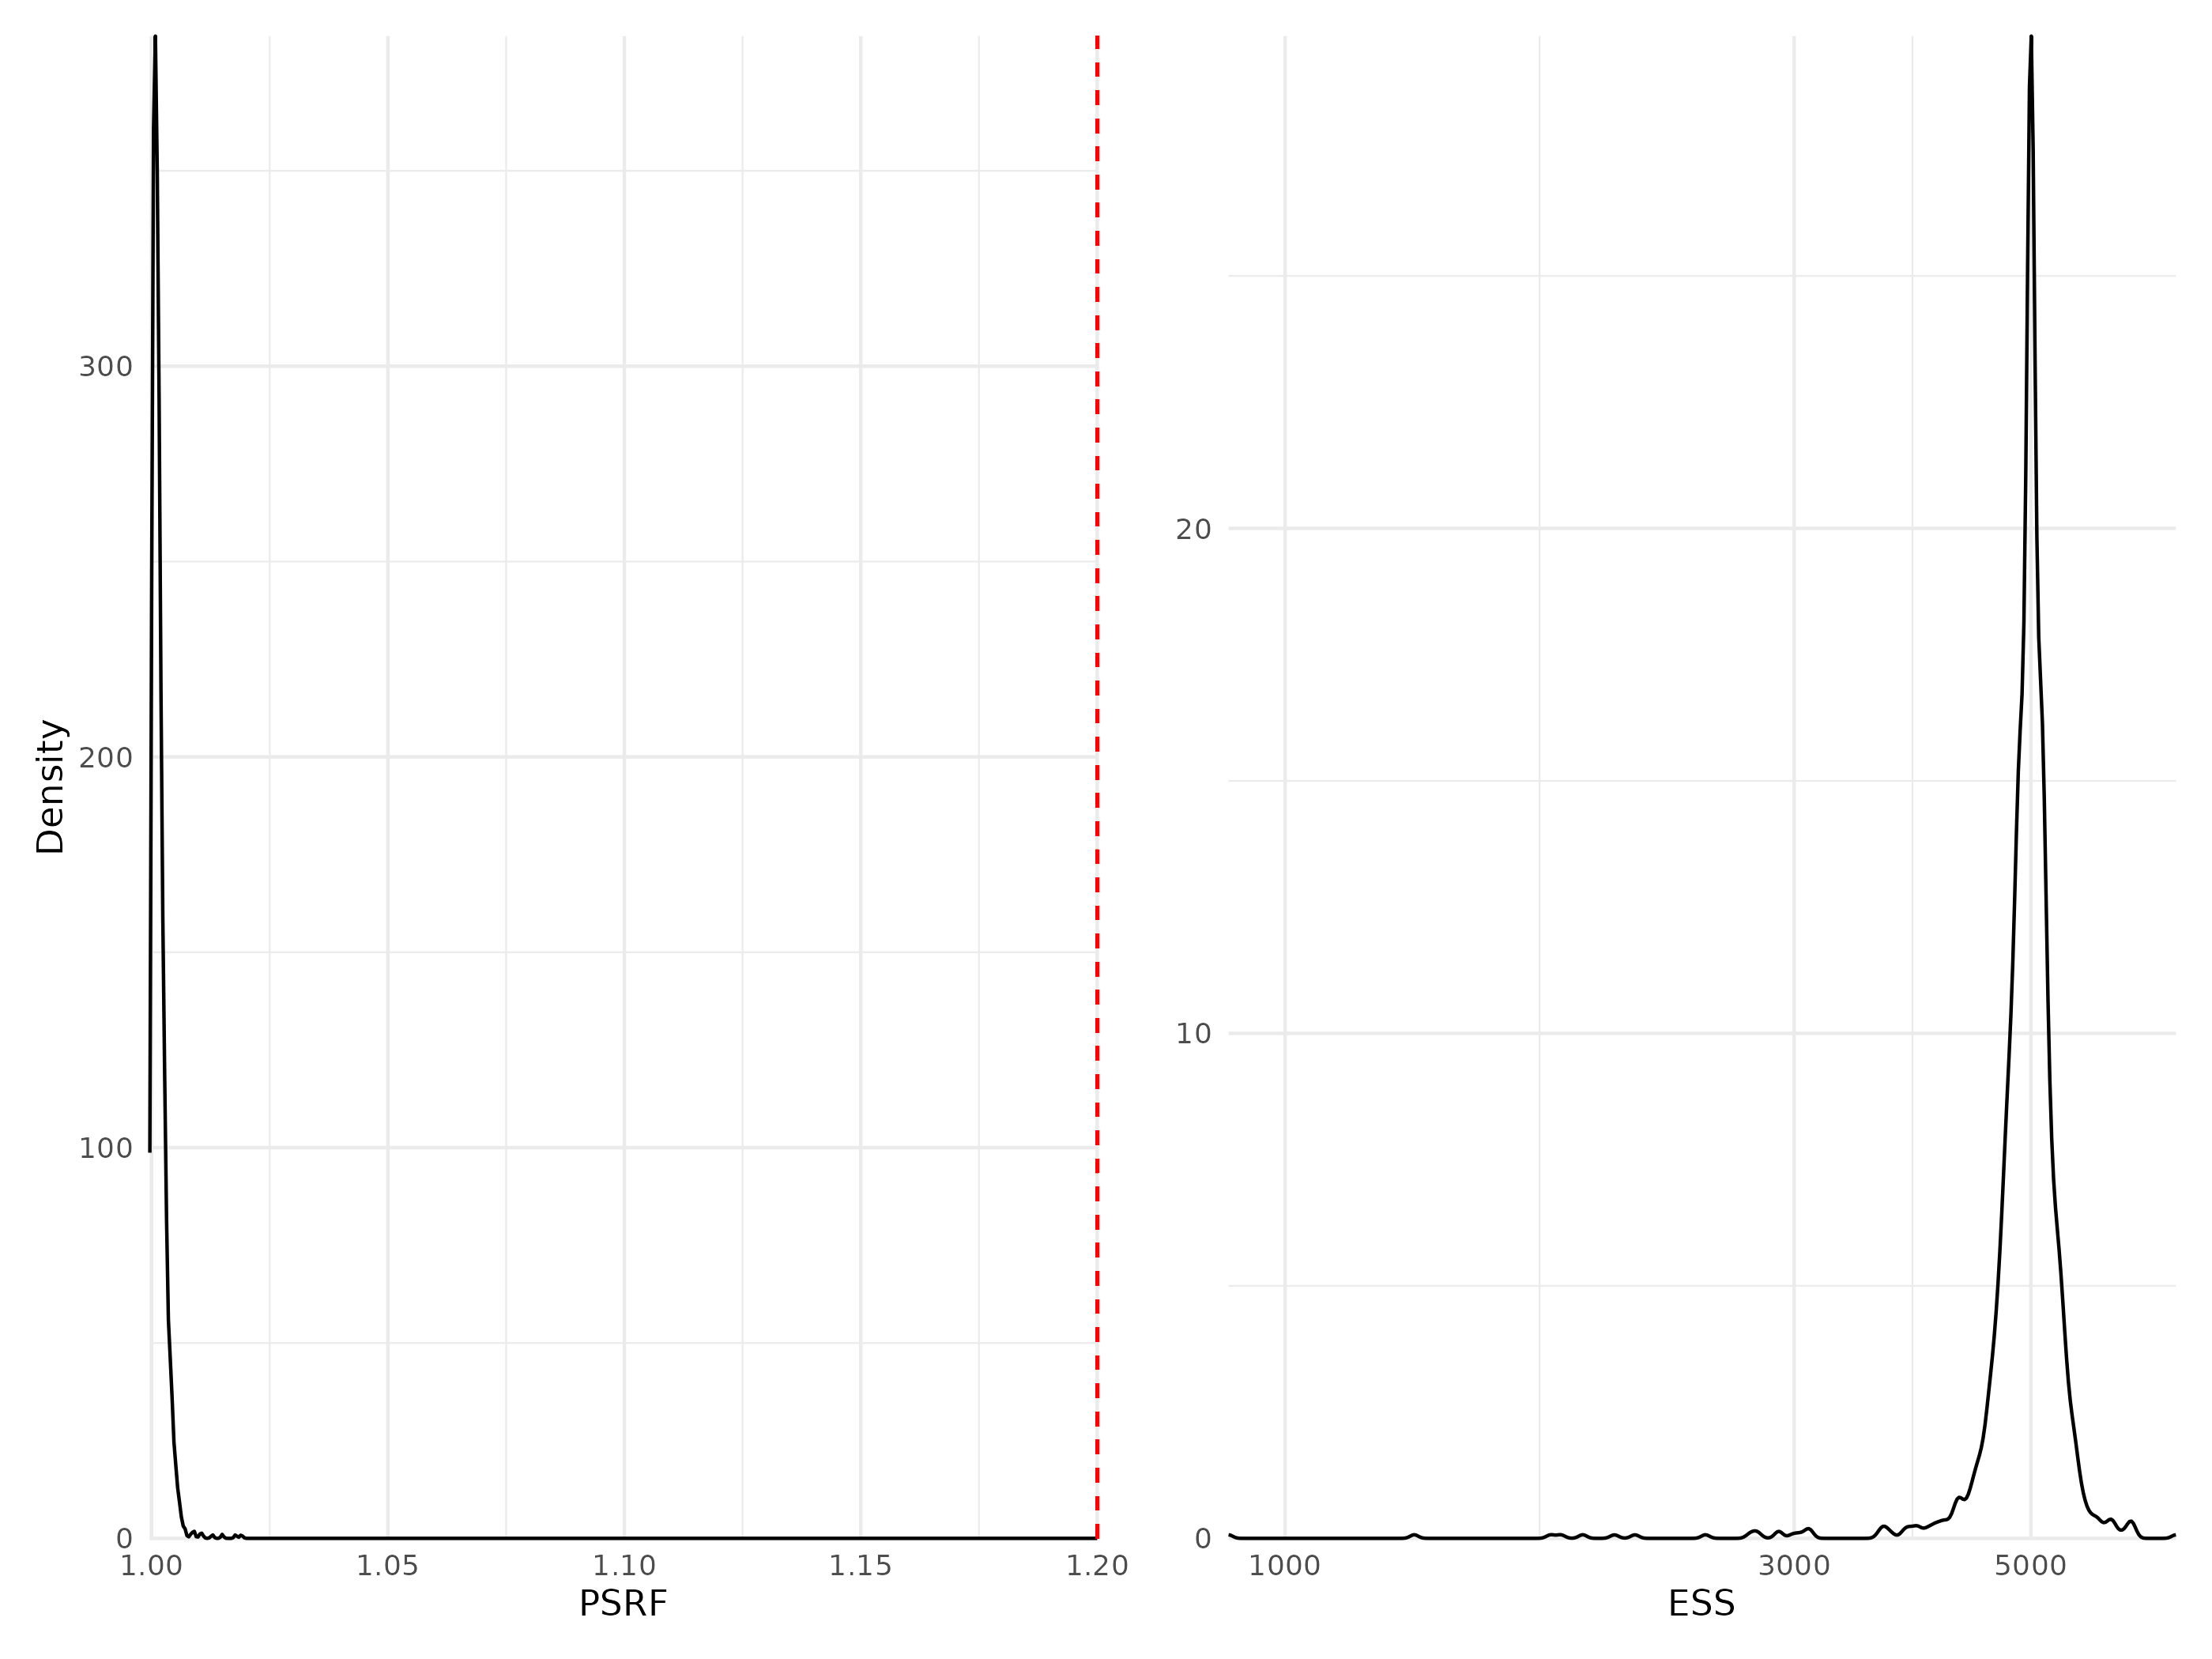
\includegraphics{03-Chapitre1/figures/supplementary/fig_supp_conv_beta_PolychaetaPhylogenyPA.png}
\caption{Density curves of potential scale reduction factors (PSRF see
\textcite{Brooks_1998}; left panel) and effective sample sizes (ESS;
right panel) for Beta regression parameters (i.e environmental
coefficients) estimated for the phylogeny model fitted with
presence/absence data. For further details see Fig.
S5.}\label{fig:chapt1phylo_pa_beta}
}
\end{figure}

\begin{figure}
\hypertarget{fig:chapt1phylo_traits_ab_beta}{%
\centering
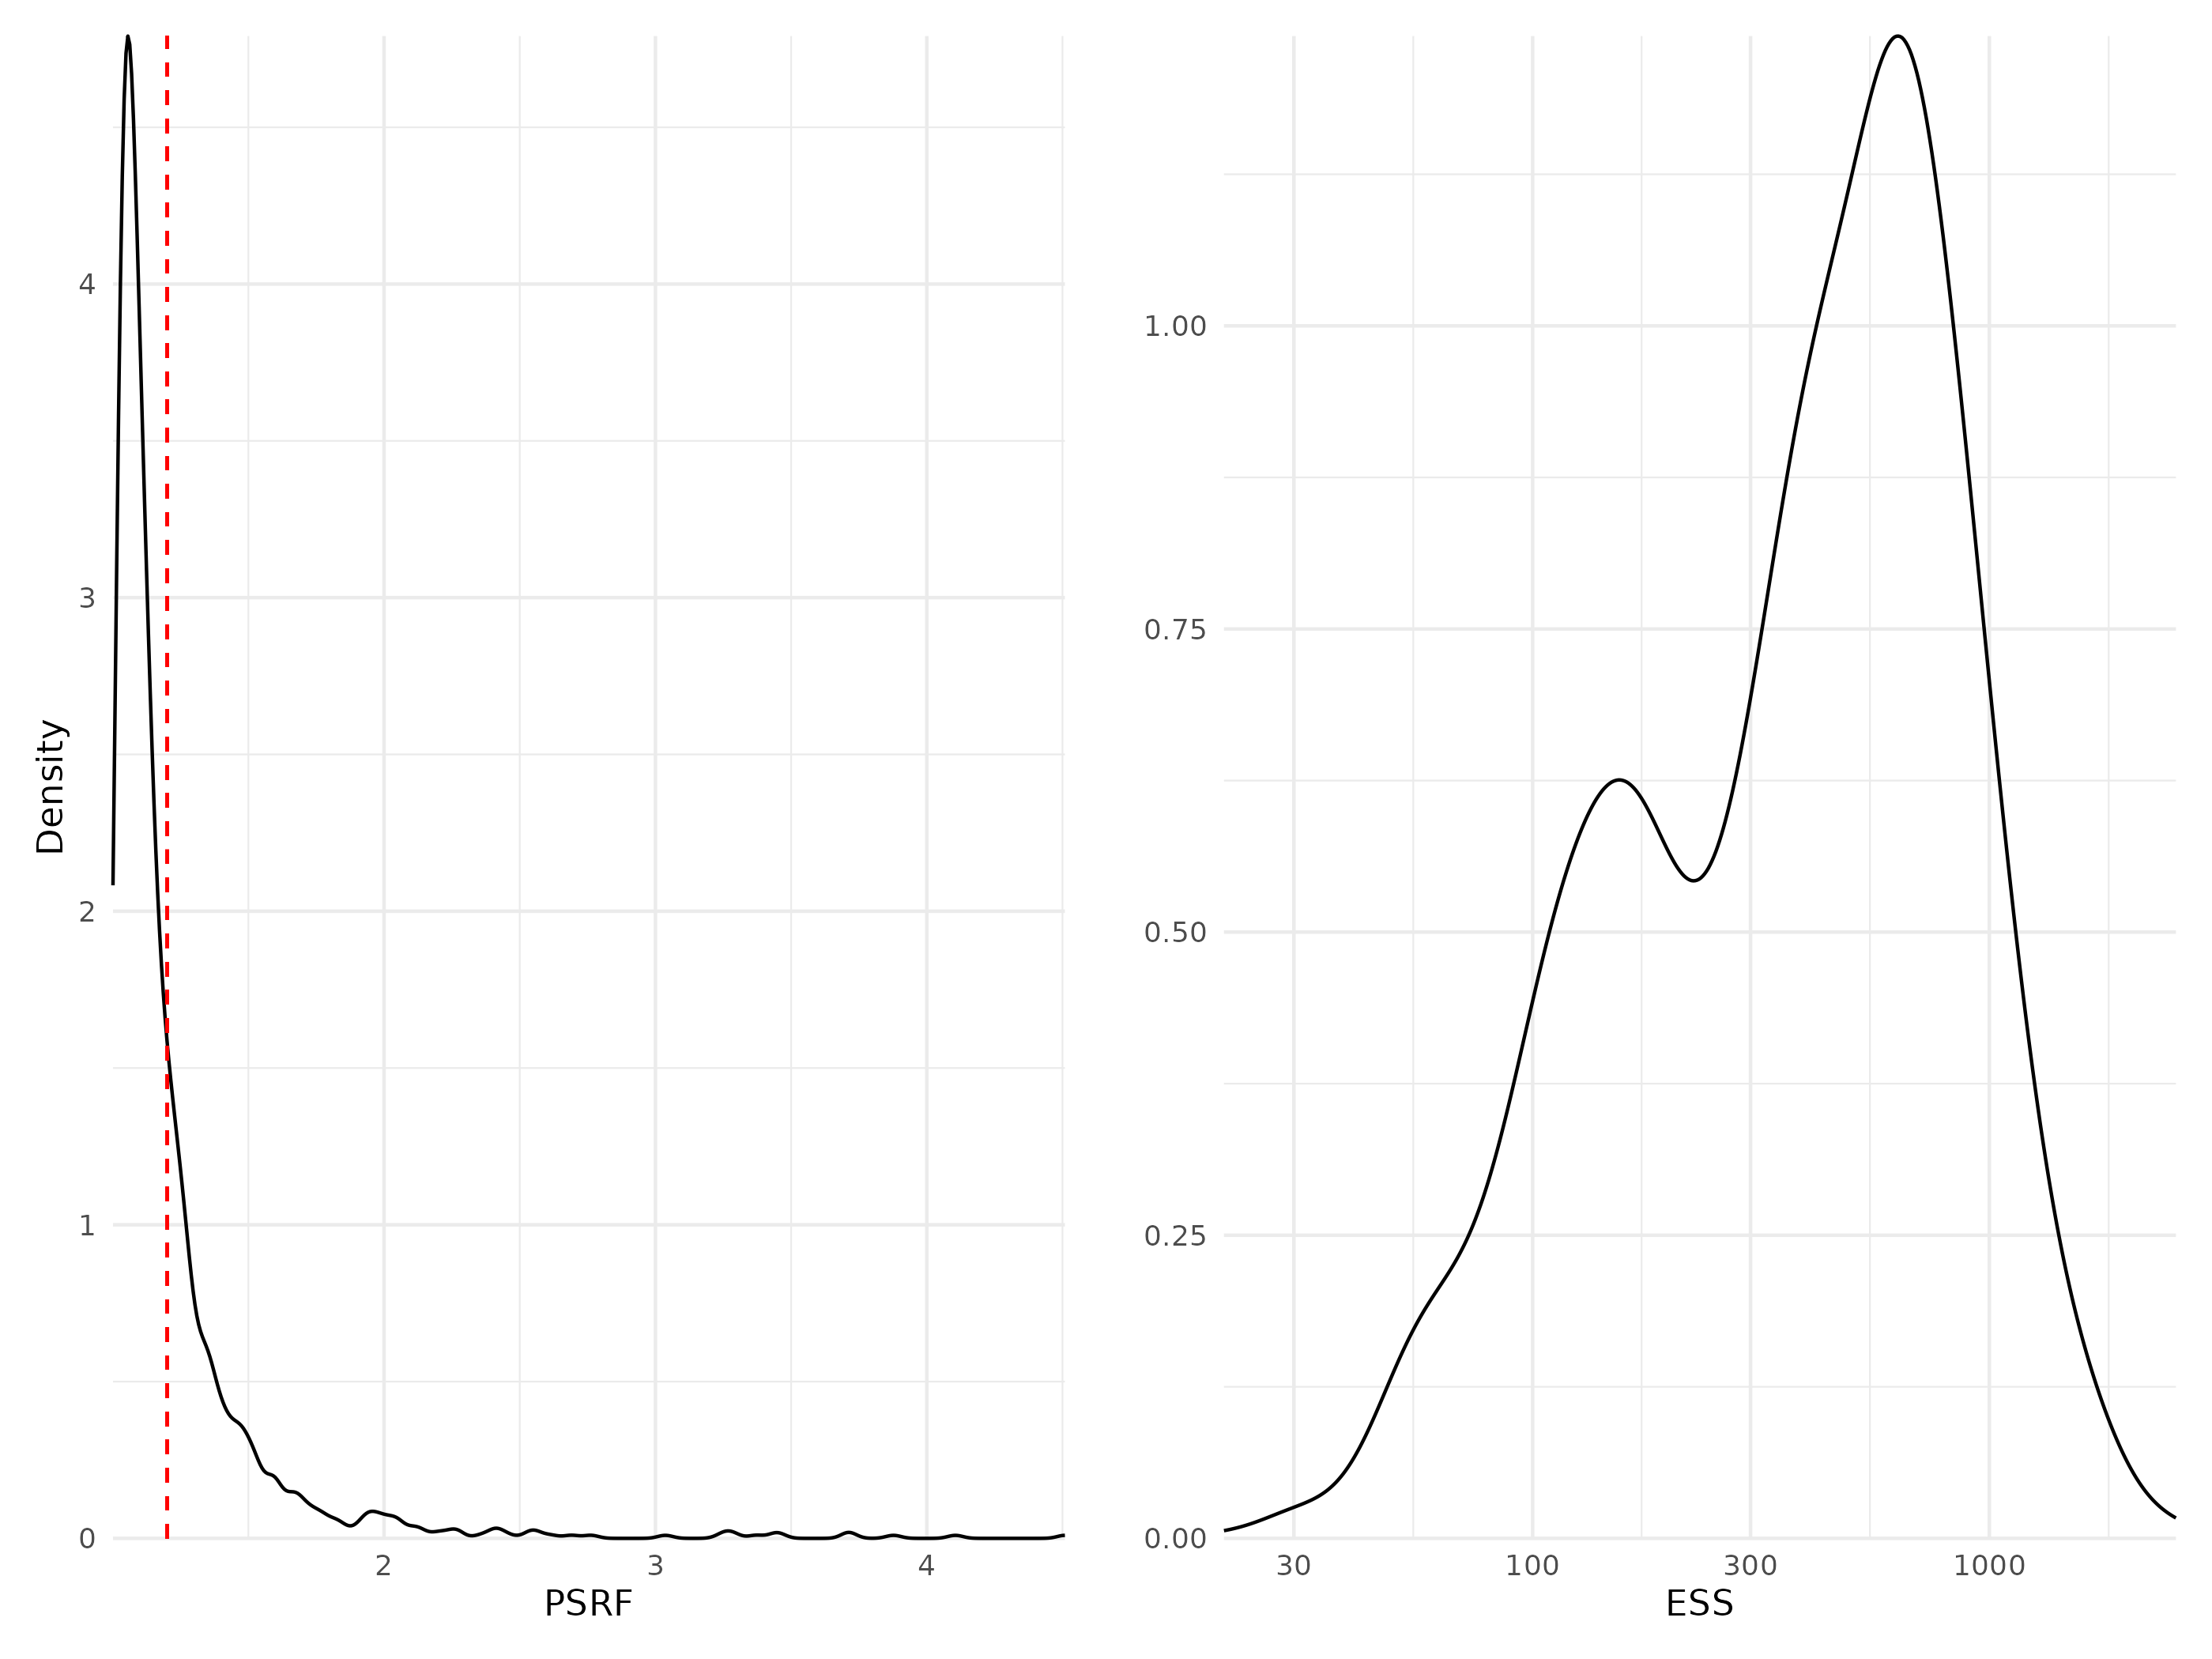
\includegraphics{03-Chapitre1/figures/supplementary/fig_supp_conv_beta_PolychaetaPhylogenyTraitsAB.png}
\caption{Density curves of potential scale reduction factors (PSRF see
\textcite{Brooks_1998}; left panel) and effective sample sizes (ESS;
right panel) for Beta regression parameters (i.e environmental
coefficients) estimated for the traits \& phylogeny model fitted with
abundance data. For further details see Fig.
S5.}\label{fig:chapt1phylo_traits_ab_beta}
}
\end{figure}

\begin{figure}
\hypertarget{fig:chapt1phylo_traits_pa_beta}{%
\centering
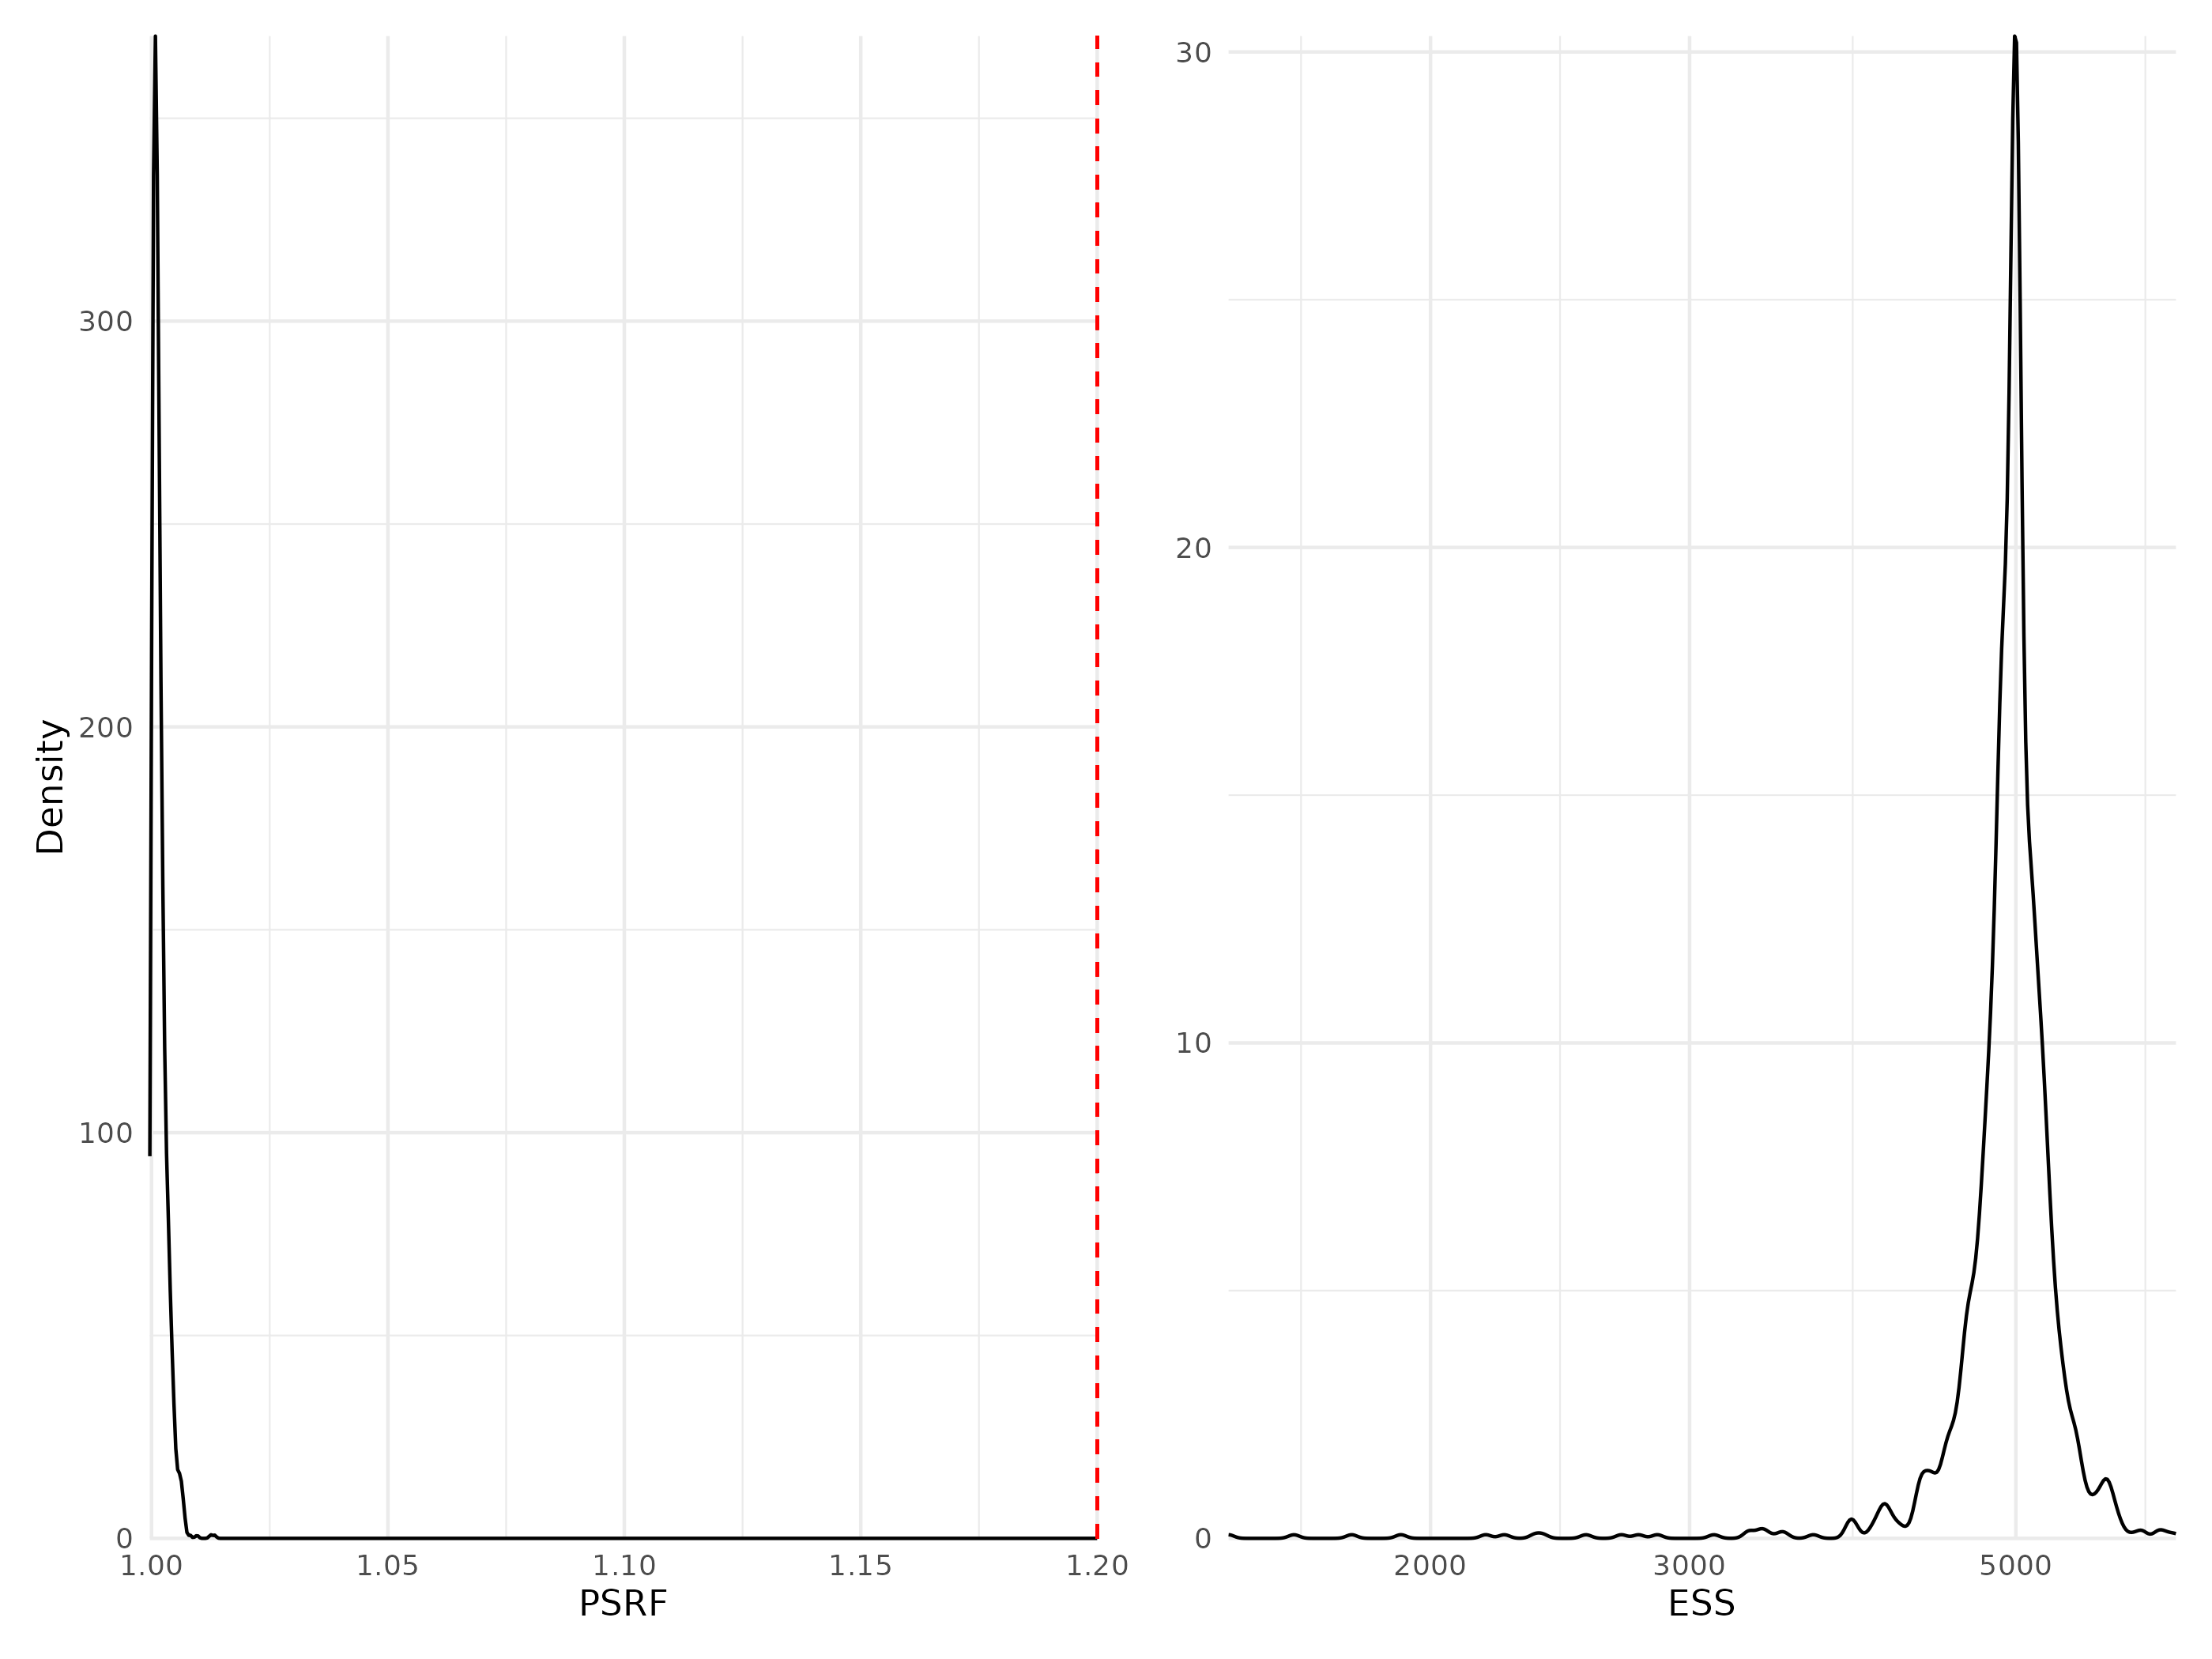
\includegraphics{03-Chapitre1/figures/supplementary/fig_supp_conv_beta_PolychaetaPhylogenyTraitsPA.png}
\caption{Density curves of potential scale reduction factors (PSRF see
\textcite{Brooks_1998}; left panel) and effective sample sizes (ESS;
right panel) for Beta regression parameters (i.e environmental
coefficients) estimated for the traits \& phylogeny model fitted with
presence/absence data. For further details see Fig.
S5.}\label{fig:chapt1phylo_traits_pa_beta}
}
\end{figure}

\begin{figure}
\hypertarget{fig:chapt1whole_comm_ab_beta}{%
\centering
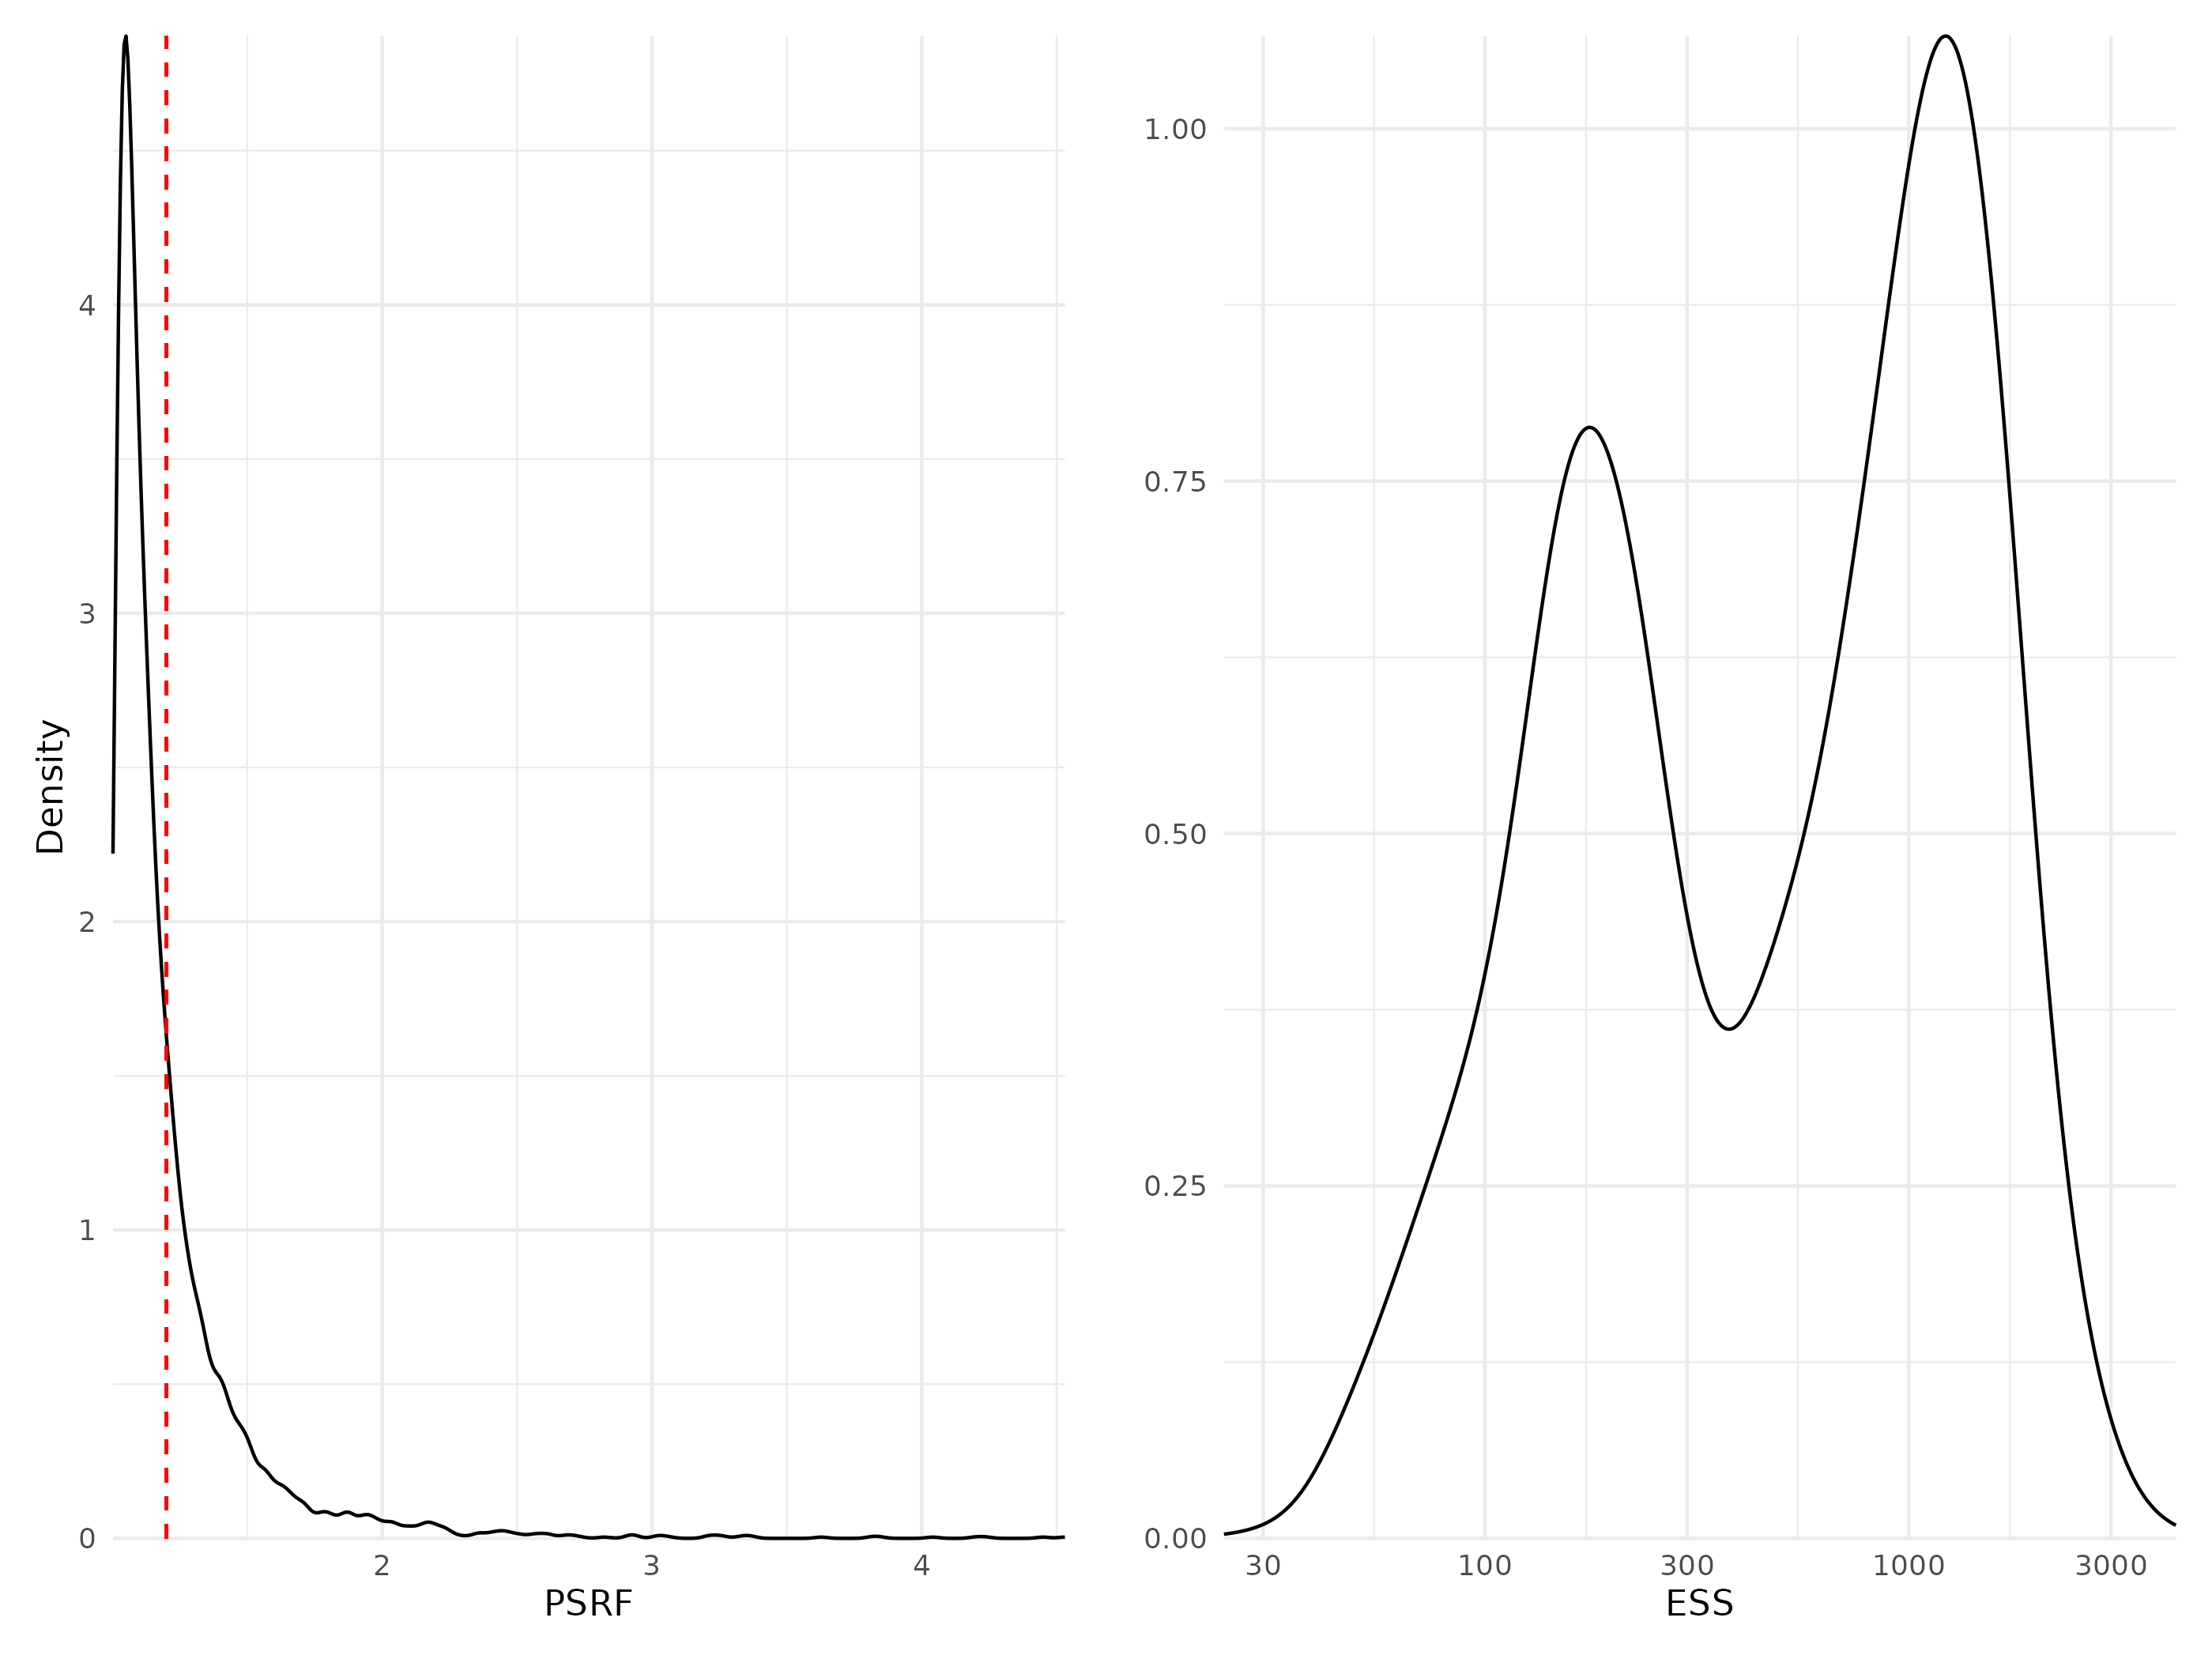
\includegraphics{03-Chapitre1/figures/supplementary/fig_supp_conv_beta_WholecommunityAB.png}
\caption{Density curves of potential scale reduction factors (PSRF see
\textcite{Brooks_1998}; left panel) and effective sample sizes (ESS;
right panel) for Beta regression parameters (i.e environmental
coefficients) estimated for the whole community model fitted with
abundance data. For further details see Fig.
S5.}\label{fig:chapt1whole_comm_ab_beta}
}
\end{figure}

\begin{figure}
\hypertarget{fig:chapt1whole_comm_pa_beta}{%
\centering
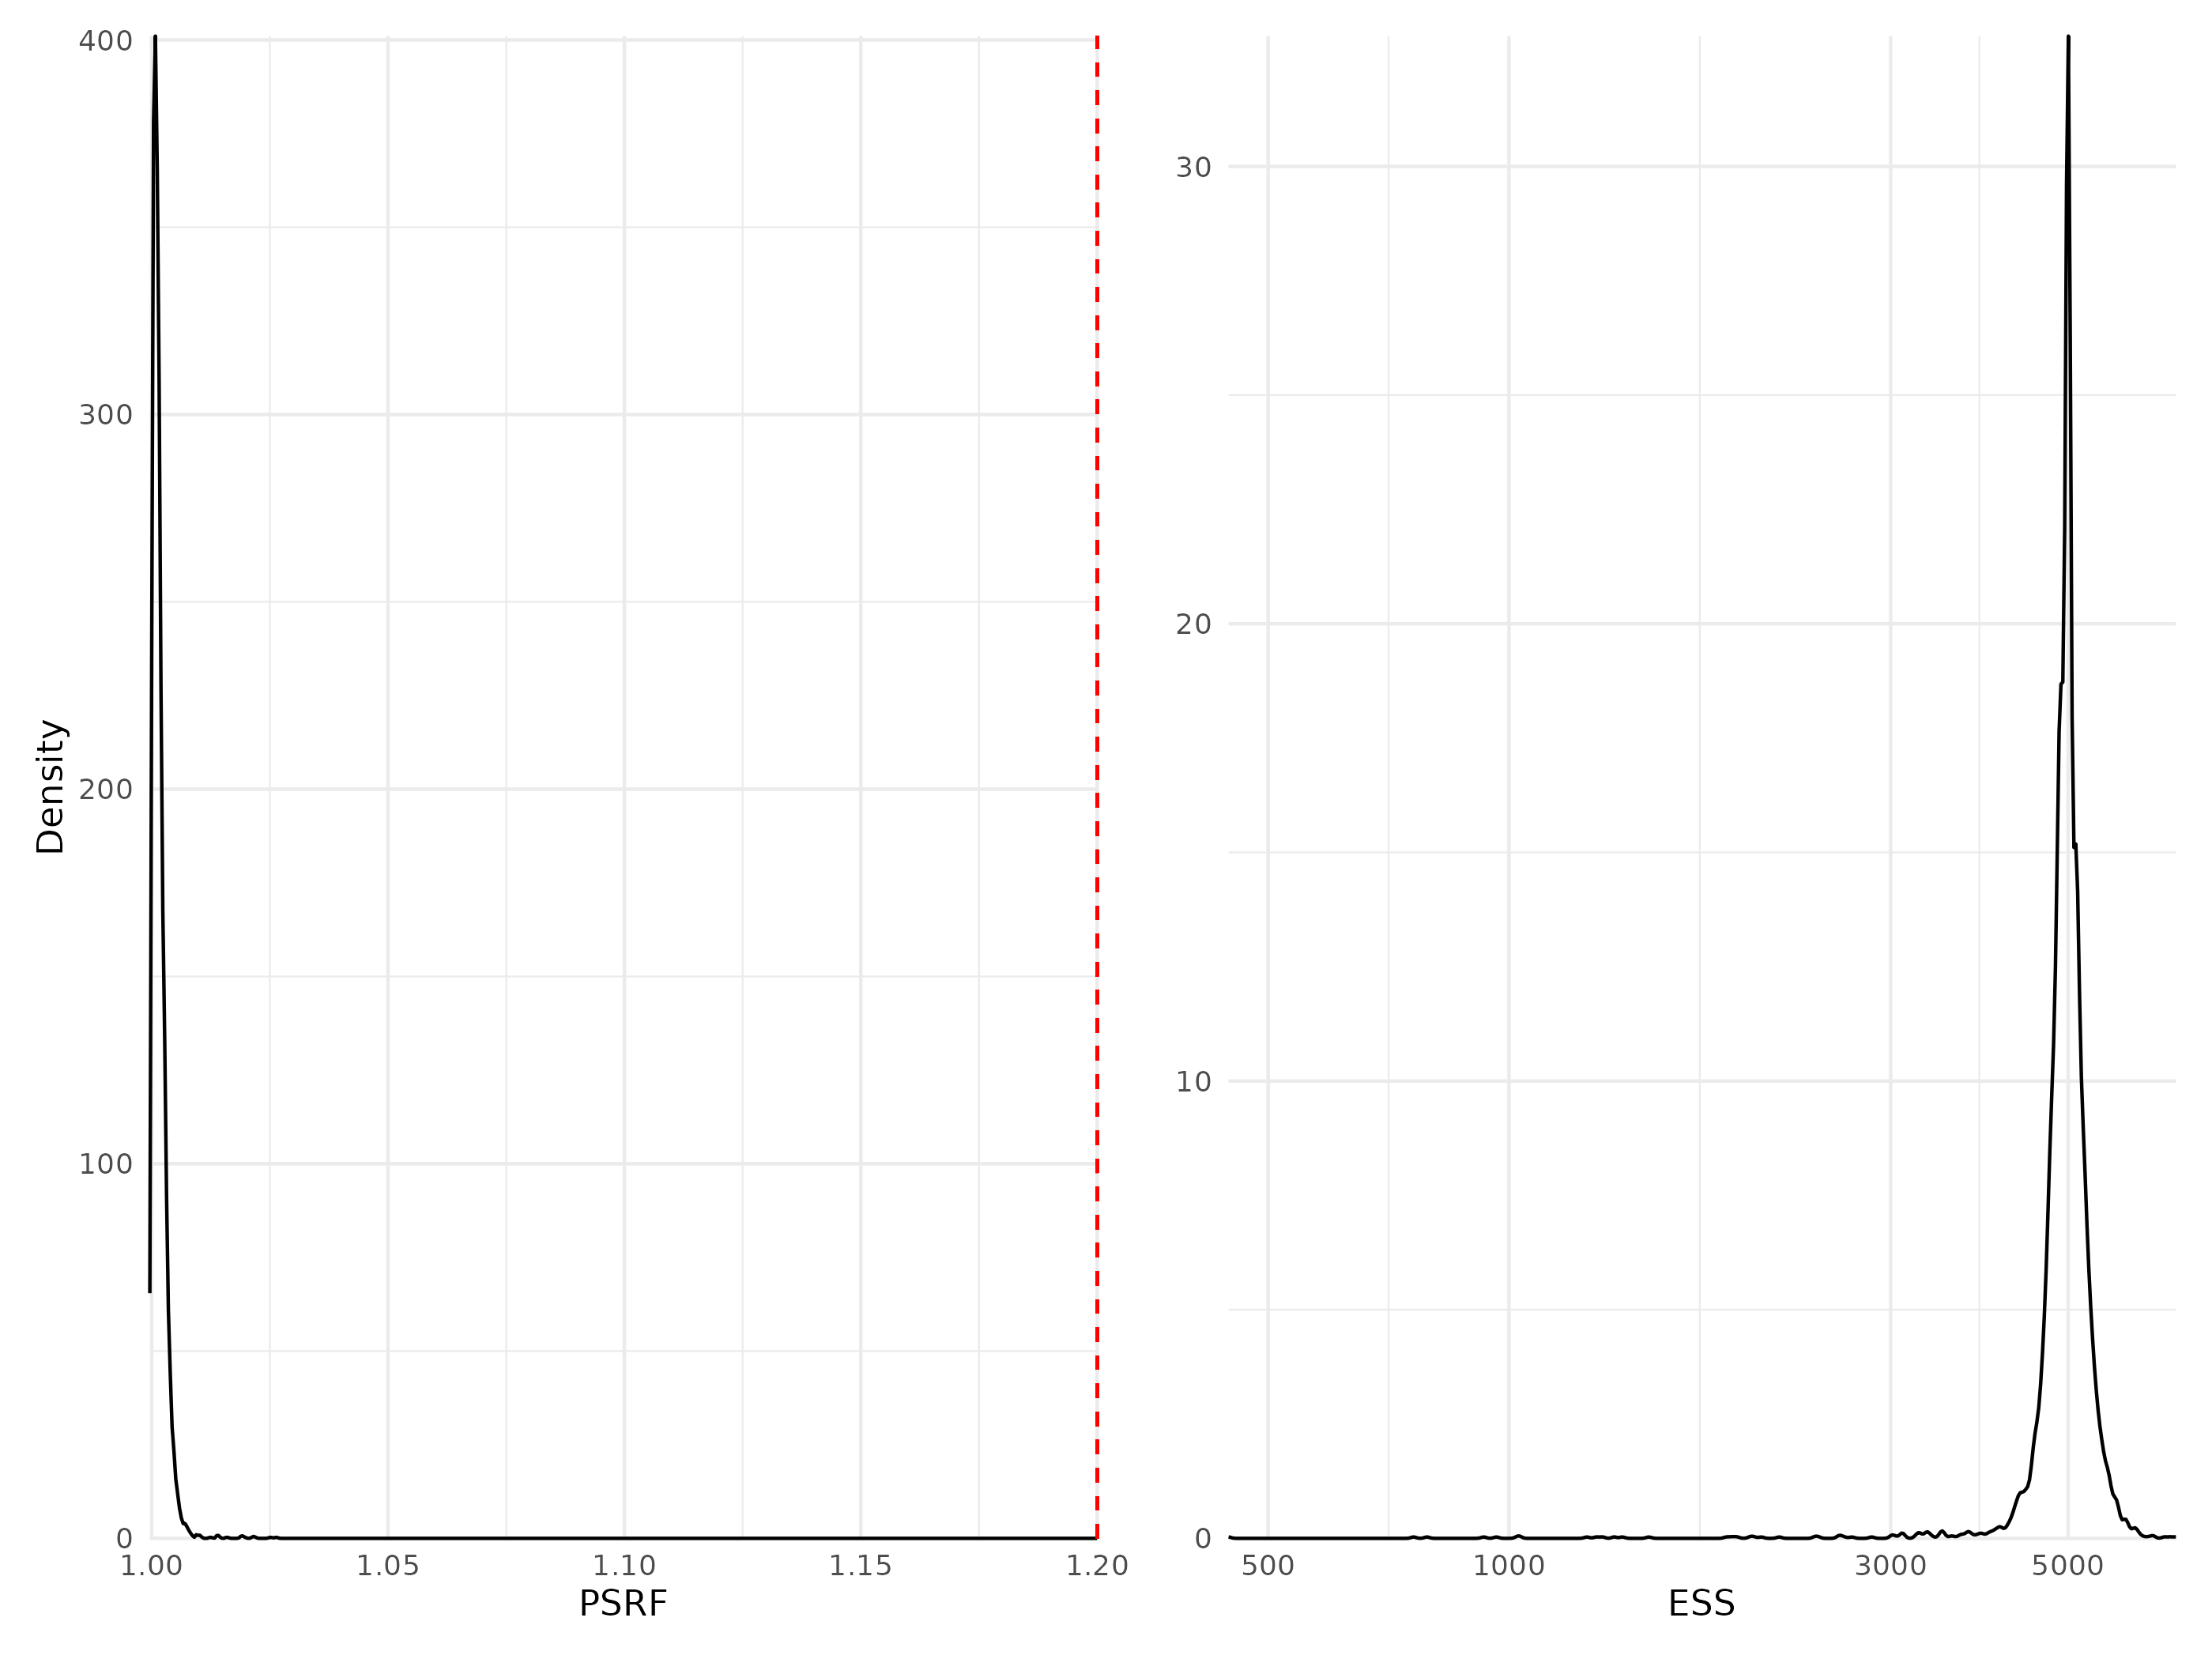
\includegraphics{03-Chapitre1/figures/supplementary/fig_supp_conv_beta_WholecommunityPA.png}
\caption{Density curves of potential scale reduction factors (PSRF see
\textcite{Brooks_1998}; left panel) and effective sample sizes (ESS;
right panel) for Beta regression parameters (i.e environmental
coefficients) estimated for the whole community model fitted with
presence/absence data. For further details see Fig.
S5.}\label{fig:chapt1whole_comm_pa_beta}
}
\end{figure}

\hypertarget{traits-coefficients}{%
\subsection*{Traits coefficients}\label{traits-coefficients}}

\hypertarget{tbl:chapt1gamma_convergence}{}
\begin{longtable}[]{@{}
  >{\raggedright\arraybackslash}p{(\columnwidth - 8\tabcolsep) * \real{0.1869}}
  >{\centering\arraybackslash}p{(\columnwidth - 8\tabcolsep) * \real{0.1869}}
  >{\raggedleft\arraybackslash}p{(\columnwidth - 8\tabcolsep) * \real{0.2243}}
  >{\raggedleft\arraybackslash}p{(\columnwidth - 8\tabcolsep) * \real{0.2056}}
  >{\raggedleft\arraybackslash}p{(\columnwidth - 8\tabcolsep) * \real{0.1963}}@{}}
\caption{\label{tbl:chapt1gamma_convergence}Potential scale reduction
factors (PSRF) and effective sample sizes (ESS) for traits regression
parameters (i.e gamma coefficients) estimated for the model including
trait information fitted either to abundance or presence-absence data.
For further details see Fig. S13 to Fig. S14.}\tabularnewline
\toprule\noalign{}
\begin{minipage}[b]{\linewidth}\raggedright
Model
\end{minipage} & \begin{minipage}[b]{\linewidth}\centering
Data type
\end{minipage} & \begin{minipage}[b]{\linewidth}\raggedleft
Number of coefficients
\end{minipage} & \begin{minipage}[b]{\linewidth}\raggedleft
PSRF (mean \(\pm\) sd)
\end{minipage} & \begin{minipage}[b]{\linewidth}\raggedleft
ESS (mean \(\pm\) sd)
\end{minipage} \\
\midrule\noalign{}
\endfirsthead
\toprule\noalign{}
\begin{minipage}[b]{\linewidth}\raggedright
Model
\end{minipage} & \begin{minipage}[b]{\linewidth}\centering
Data type
\end{minipage} & \begin{minipage}[b]{\linewidth}\raggedleft
Number of coefficients
\end{minipage} & \begin{minipage}[b]{\linewidth}\raggedleft
PSRF (mean \(\pm\) sd)
\end{minipage} & \begin{minipage}[b]{\linewidth}\raggedleft
ESS (mean \(\pm\) sd)
\end{minipage} \\
\midrule\noalign{}
\endhead
\bottomrule\noalign{}
\endlastfoot
Traits \& Phylogeny & Abundance & 60 & 1.08 \(\pm\) 0.092 & 1232 \(\pm\)
1209 \\
Traits \& Phylogeny & Presence/Absence & 60 & 1.00 \(\pm\) 0.001 & 13227
\(\pm\) 1897 \\
\end{longtable}

\begin{figure}
\hypertarget{fig:chapt1phylo_traits_ab_gamma}{%
\centering
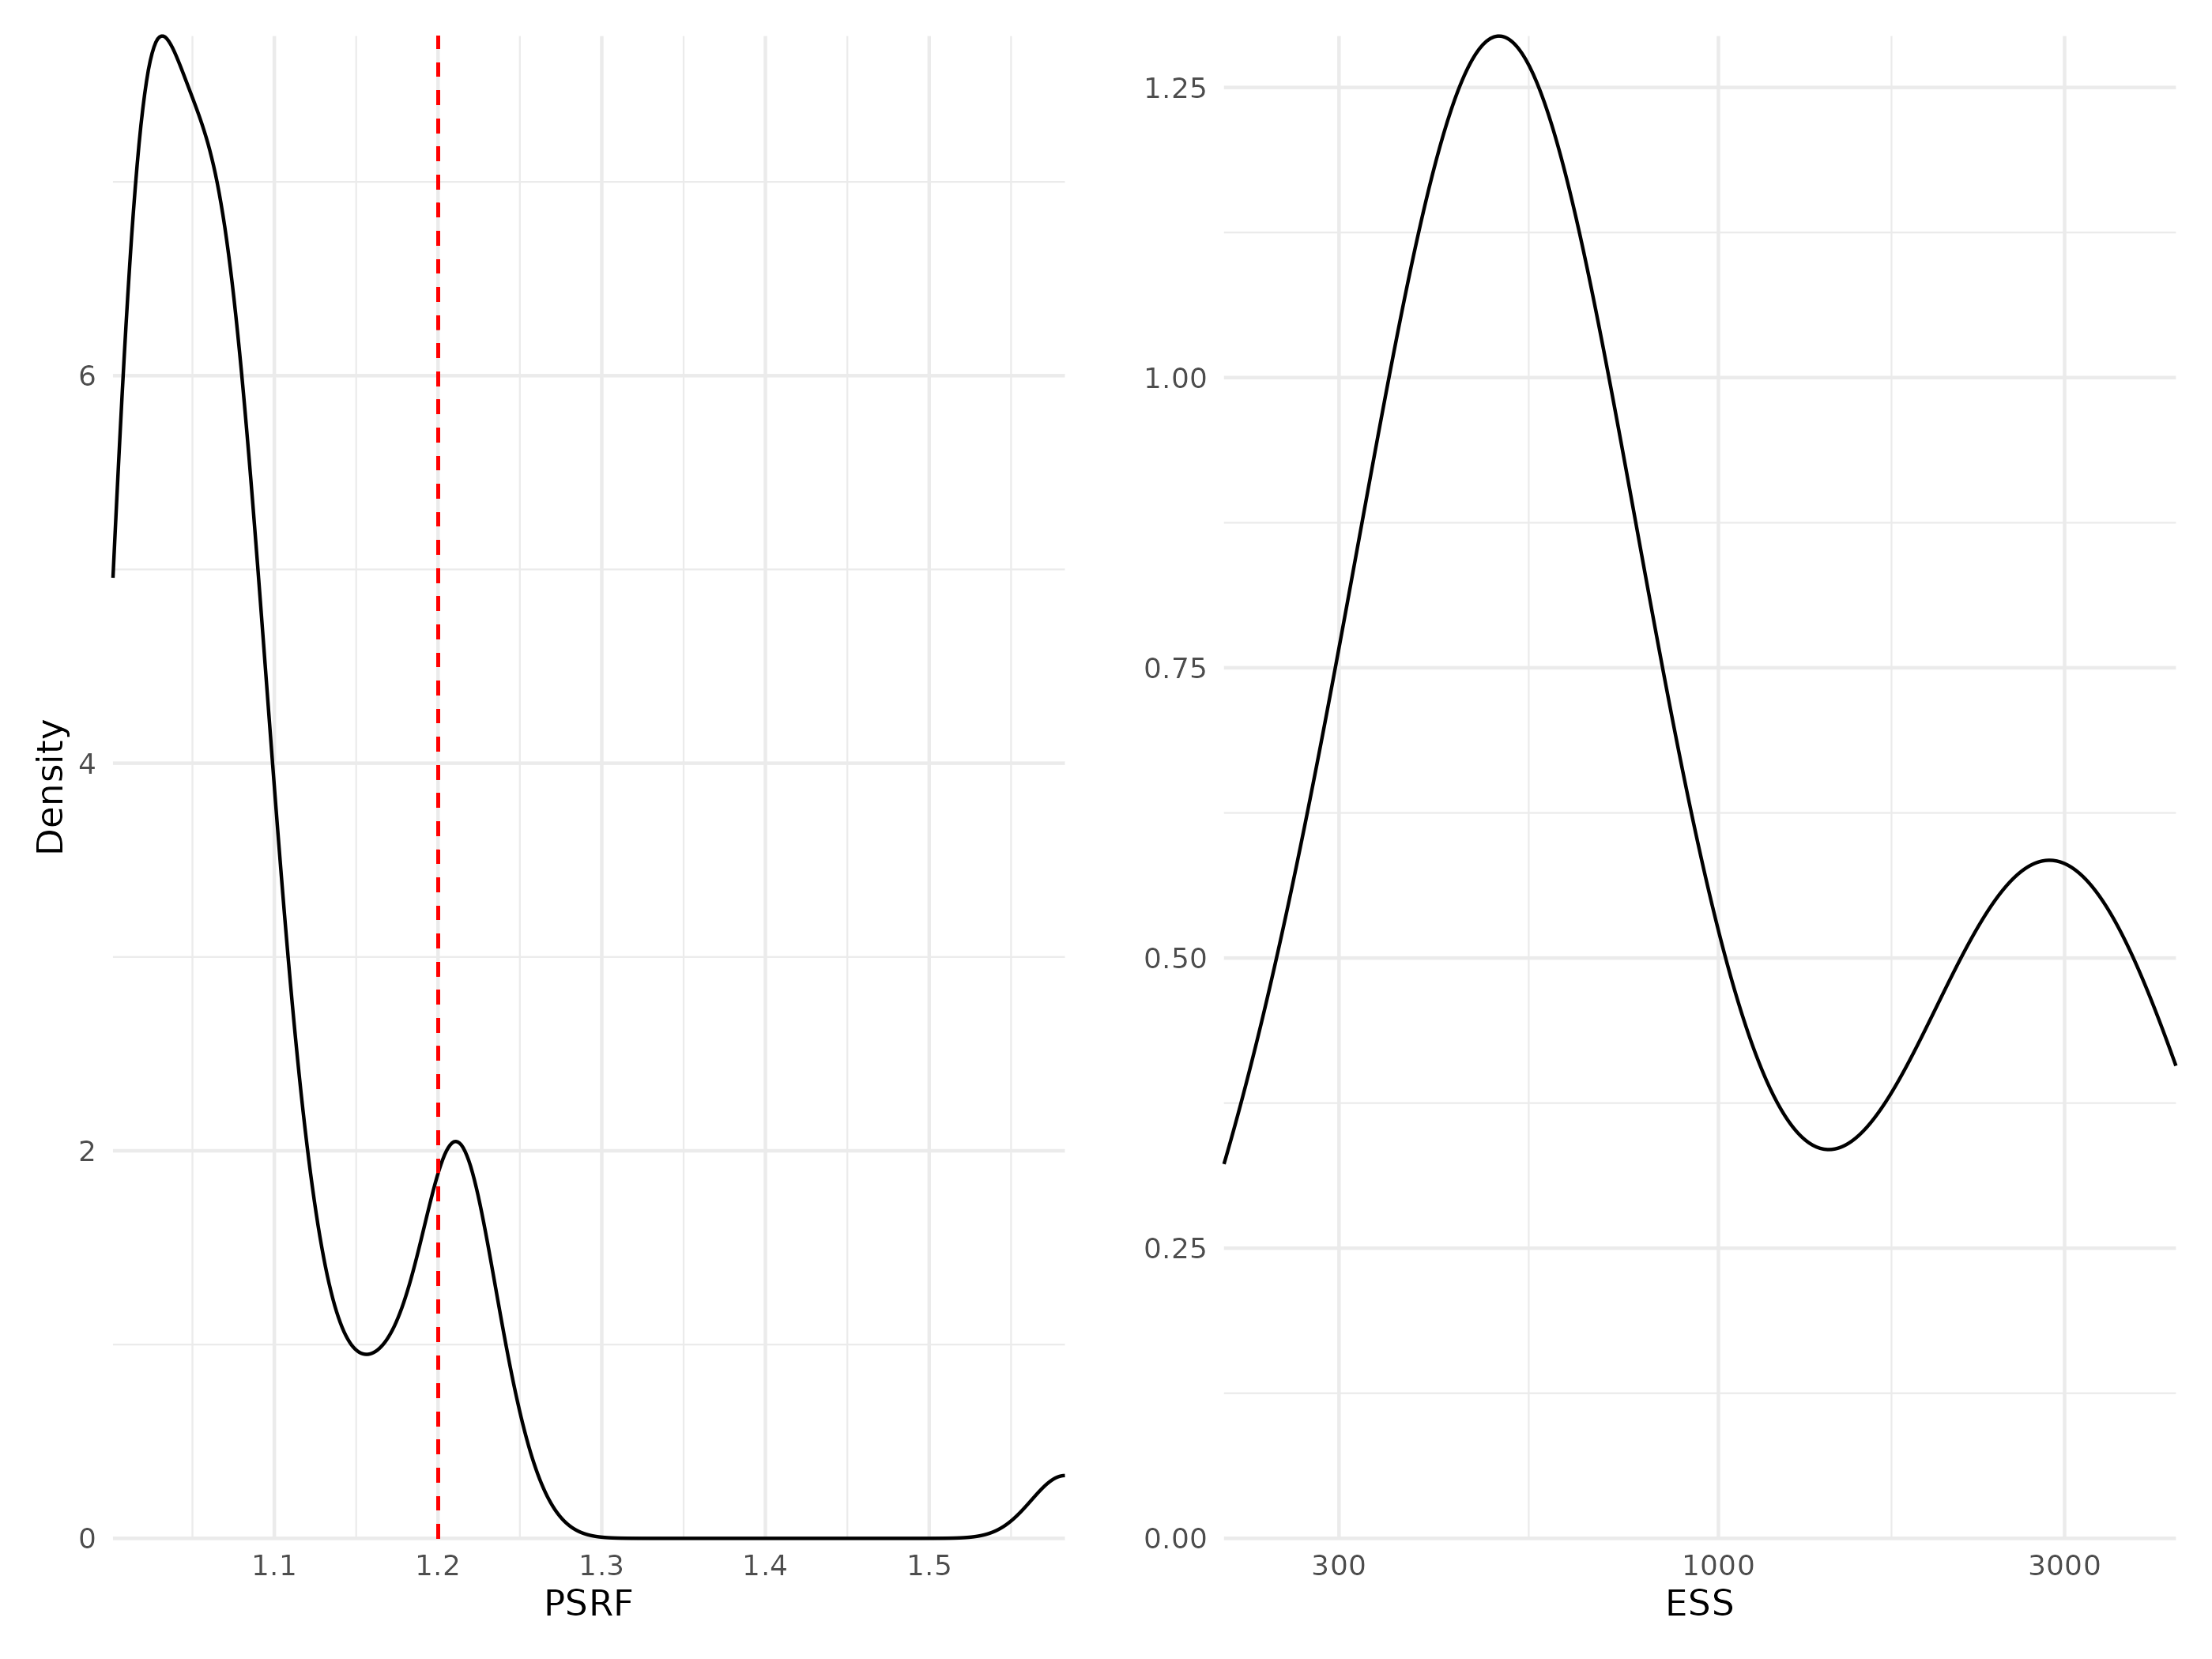
\includegraphics{03-Chapitre1/figures/supplementary/fig_supp_conv_gamma_PolychaetaPhylogenyTraitsAB.png}
\caption{Density curves of potential scale reduction factors (PSRF see
\textcite{Brooks_1998}; left panel) and effective sample sizes (ESS;
right panel) for Gamma regression parameters (i.e coefficients
associated with trait-environment interactions, modeling how species
traits influence their niches) estimated for the traits \& phylogeny
model fitted with abundance data. For further details see Fig.
S5.}\label{fig:chapt1phylo_traits_ab_gamma}
}
\end{figure}

\begin{figure}
\hypertarget{fig:chapt1phylo_traits_pa_gamma}{%
\centering
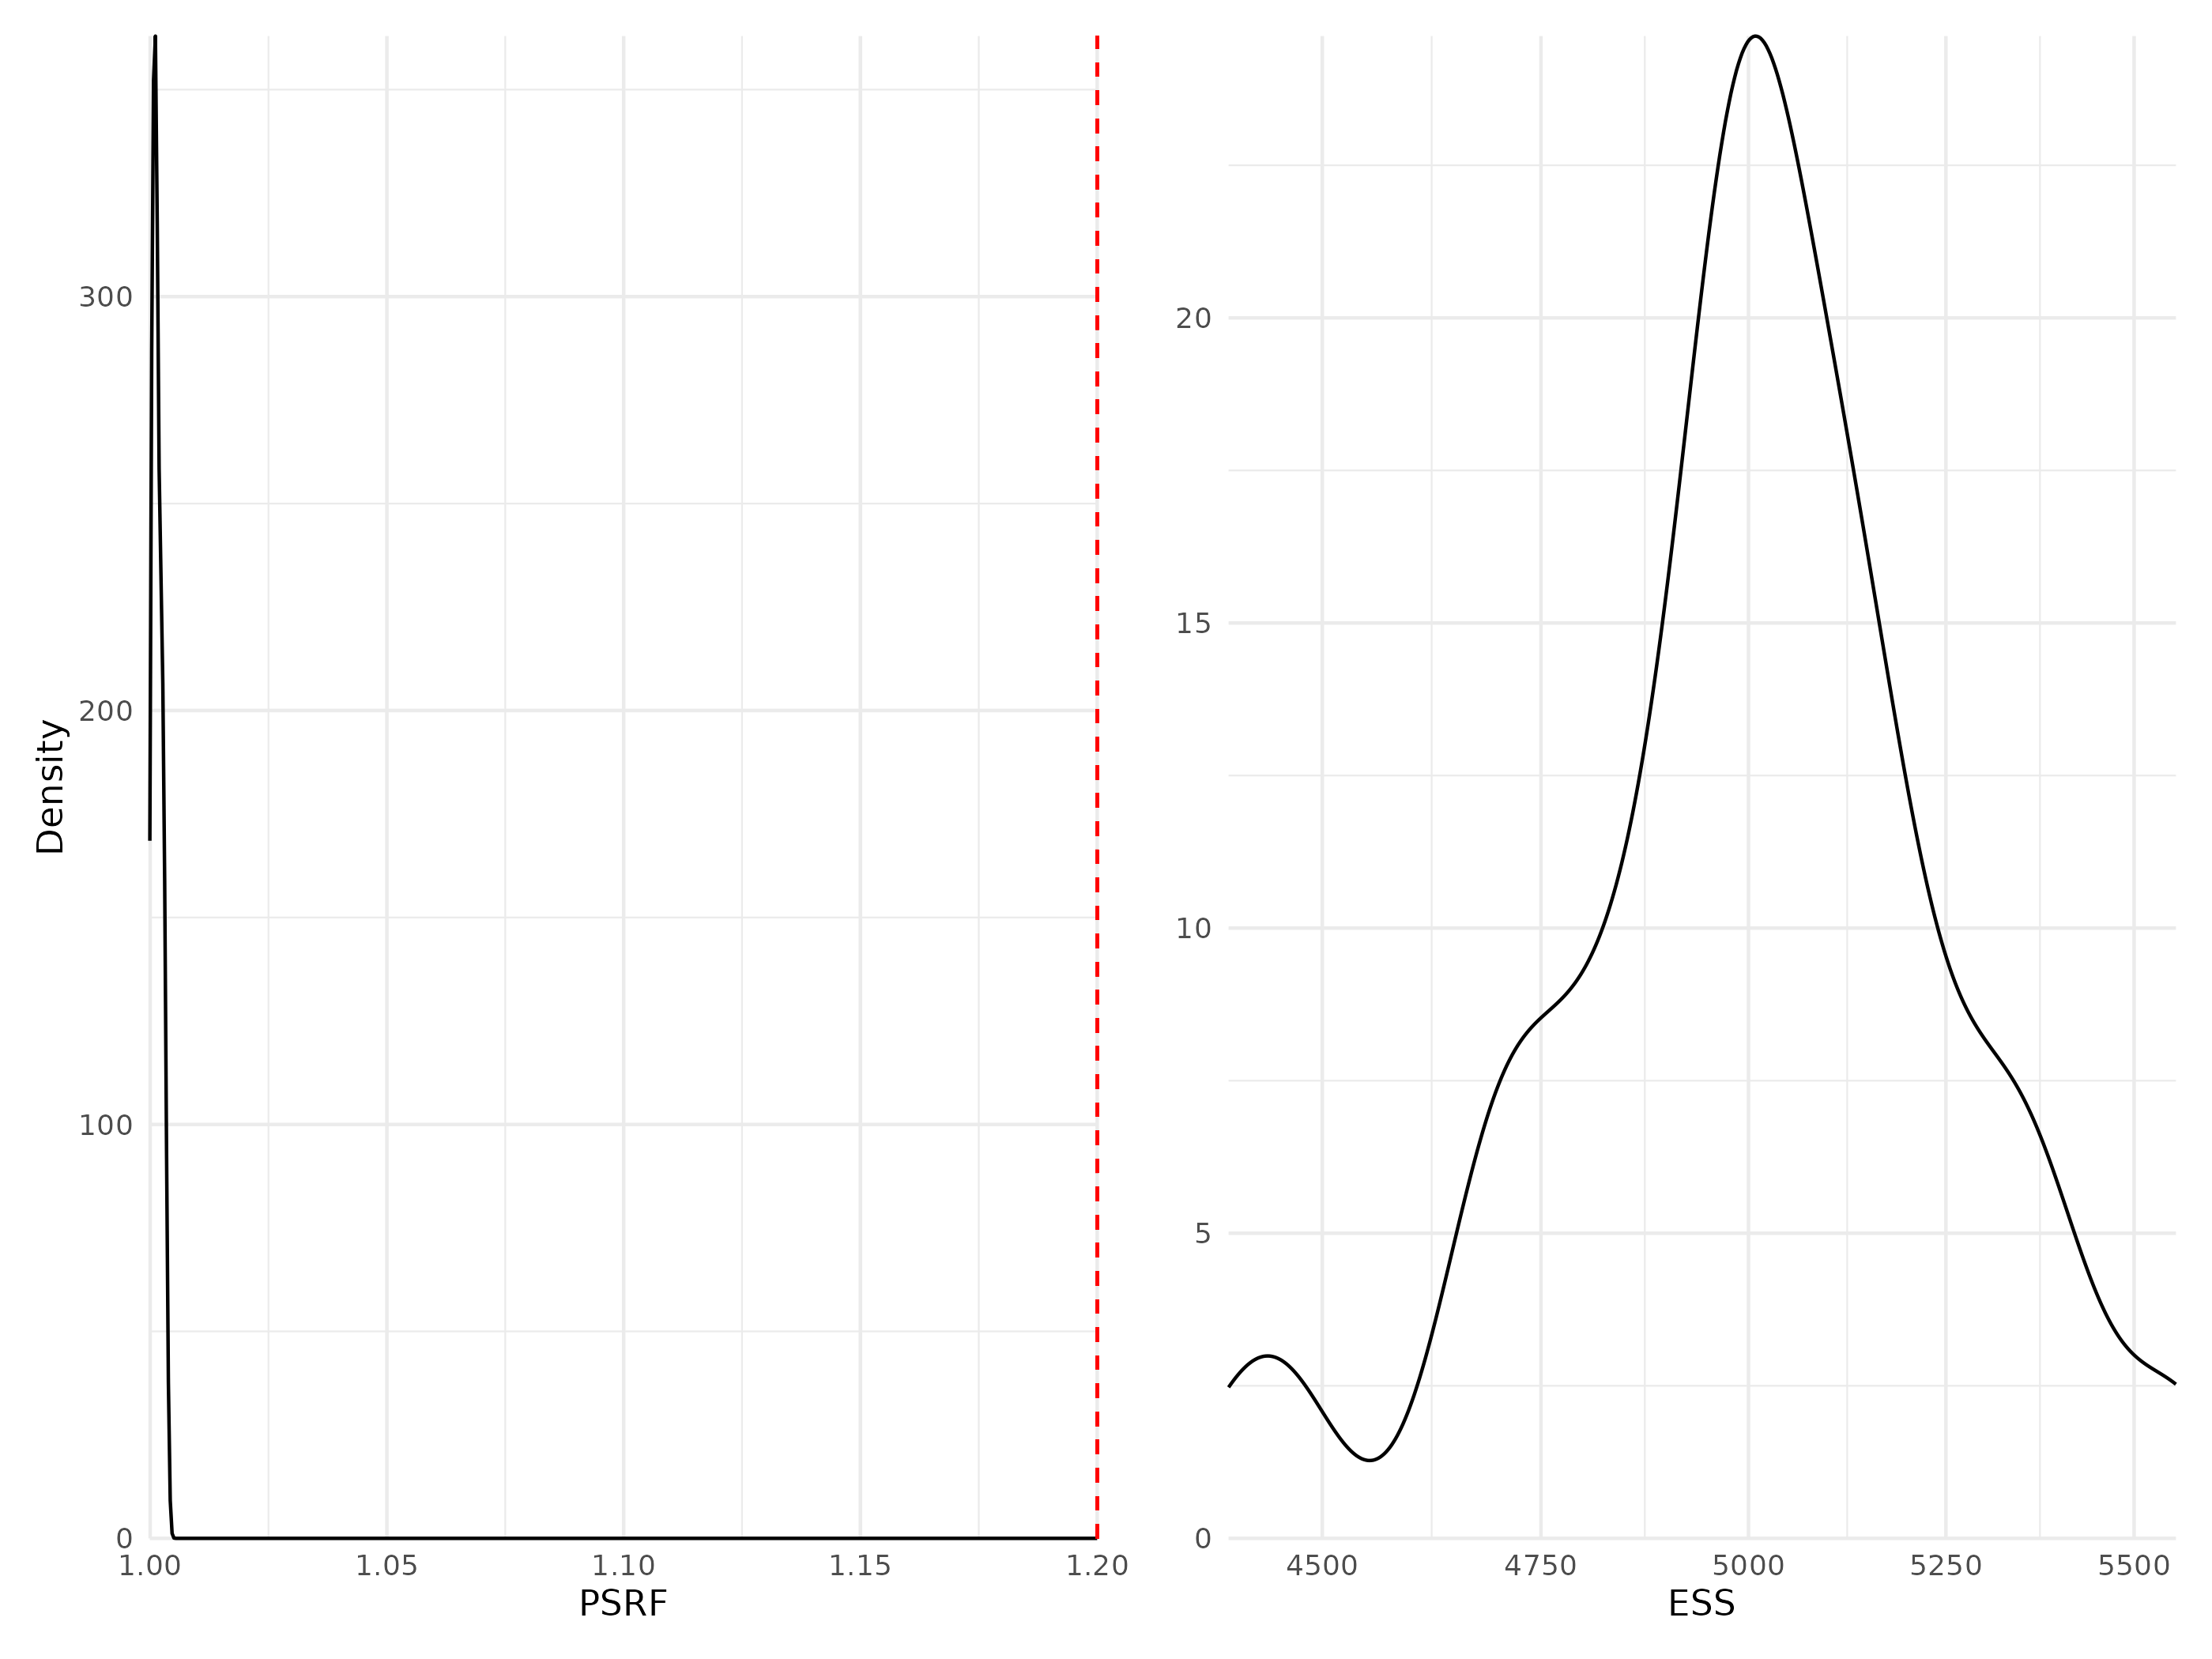
\includegraphics{03-Chapitre1/figures/supplementary/fig_supp_conv_gamma_PolychaetaPhylogenyTraitsPA.png}
\caption{Density curves of potential scale reduction factors (PSRF see
\textcite{Brooks_1998}; left panel) and effective sample sizes (ESS;
right panel) for Gamma regression parameters (i.e coefficients
associated with trait-environment interactions, modeling how species
traits influence their niches) estimated for the traits \& phylogeny
model fitted with presence/absence data. For further details see Fig.
S5.}\label{fig:chapt1phylo_traits_pa_gamma}
}
\end{figure}

\hypertarget{phylogeny-coefficients}{%
\subsection*{Phylogeny coefficients}\label{phylogeny-coefficients}}

\hypertarget{tbl:chapt1rho_convergence}{}
\begin{longtable}[]{@{}
  >{\raggedright\arraybackslash}p{(\columnwidth - 8\tabcolsep) * \real{0.2619}}
  >{\centering\arraybackslash}p{(\columnwidth - 8\tabcolsep) * \real{0.2143}}
  >{\centering\arraybackslash}p{(\columnwidth - 8\tabcolsep) * \real{0.2857}}
  >{\raggedleft\arraybackslash}p{(\columnwidth - 8\tabcolsep) * \real{0.1071}}
  >{\raggedleft\arraybackslash}p{(\columnwidth - 8\tabcolsep) * \real{0.1310}}@{}}
\caption{\label{tbl:chapt1rho_convergence}Potential scale reduction
factors (PSRF) and effective sample sizes (ESS) for rho regression
parameters (i.e phylogeny coefficient) estimated for the two models
including phylogenetic information (TrPh and Ph).}\tabularnewline
\toprule\noalign{}
\begin{minipage}[b]{\linewidth}\raggedright
Model
\end{minipage} & \begin{minipage}[b]{\linewidth}\centering
Data type
\end{minipage} & \begin{minipage}[b]{\linewidth}\centering
Number of coefficients
\end{minipage} & \begin{minipage}[b]{\linewidth}\raggedleft
PSRF
\end{minipage} & \begin{minipage}[b]{\linewidth}\raggedleft
ESS
\end{minipage} \\
\midrule\noalign{}
\endfirsthead
\toprule\noalign{}
\begin{minipage}[b]{\linewidth}\raggedright
Model
\end{minipage} & \begin{minipage}[b]{\linewidth}\centering
Data type
\end{minipage} & \begin{minipage}[b]{\linewidth}\centering
Number of coefficients
\end{minipage} & \begin{minipage}[b]{\linewidth}\raggedleft
PSRF
\end{minipage} & \begin{minipage}[b]{\linewidth}\raggedleft
ESS
\end{minipage} \\
\midrule\noalign{}
\endhead
\bottomrule\noalign{}
\endlastfoot
Phylogeny & Abundance & 1 & 1.07 & 649 \\
Phylogeny & Presence/Absence & 1 & 1.00 & 9349 \\
Traits \& Phylogeny & Abundance & 1 & 1.15 & 757 \\
Traits \& Phylogeny & Presence/Absence & 1 & 1.00 & 5000 \\
\end{longtable}

\hypertarget{link-between-model-convergence-and-species-response-curves}{%
\subsection*{Link between model convergence and species response
curves}\label{link-between-model-convergence-and-species-response-curves}}

\begin{figure}
\hypertarget{fig:chapt1supp15}{%
\centering
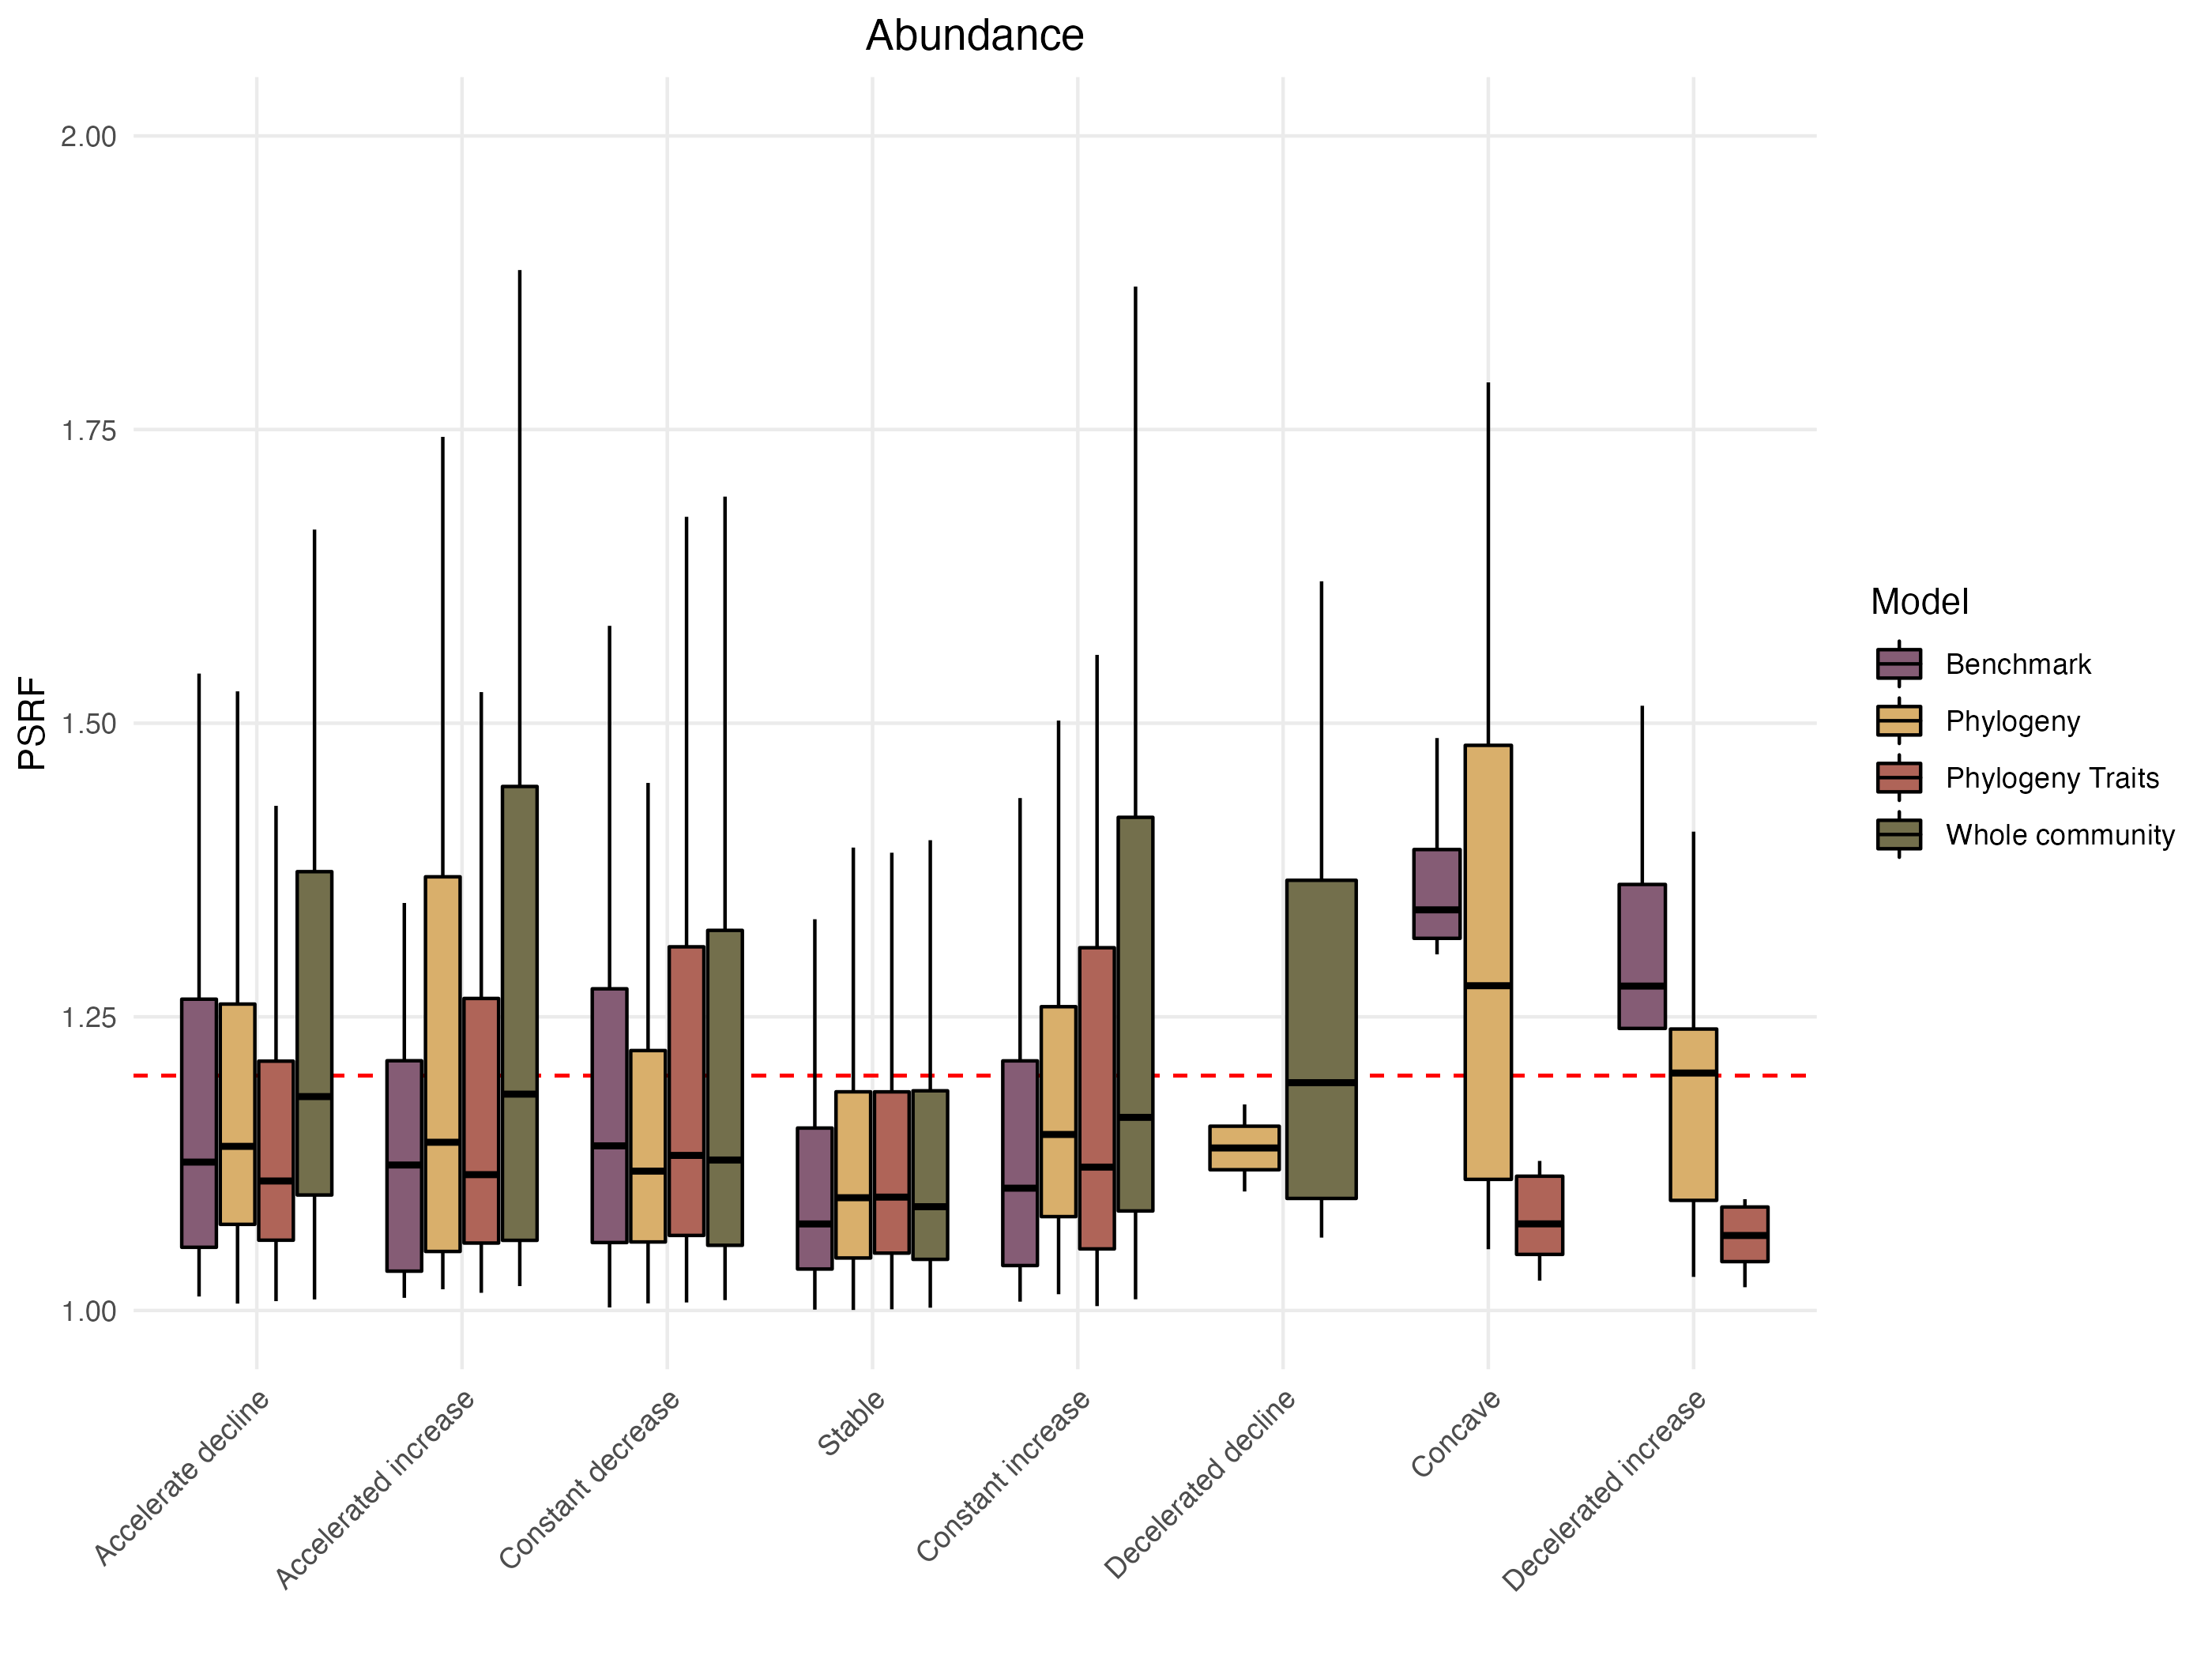
\includegraphics{03-Chapitre1/figures/supplementary/fig_supp15.png}
\caption{Distribution of the Potential scale reduction factors (PSRF) as
a function of the different shapes of the response curves classified
following the methodology proposed by \textcite{Rigal_2020} methods (see
section ``Assessing model performance and interpretability'' for more
details on the calculation methodology). Results for models fitted with
abundance data.}\label{fig:chapt1supp15}
}
\end{figure}

\begin{figure}
\hypertarget{fig:chapt1supp16}{%
\centering
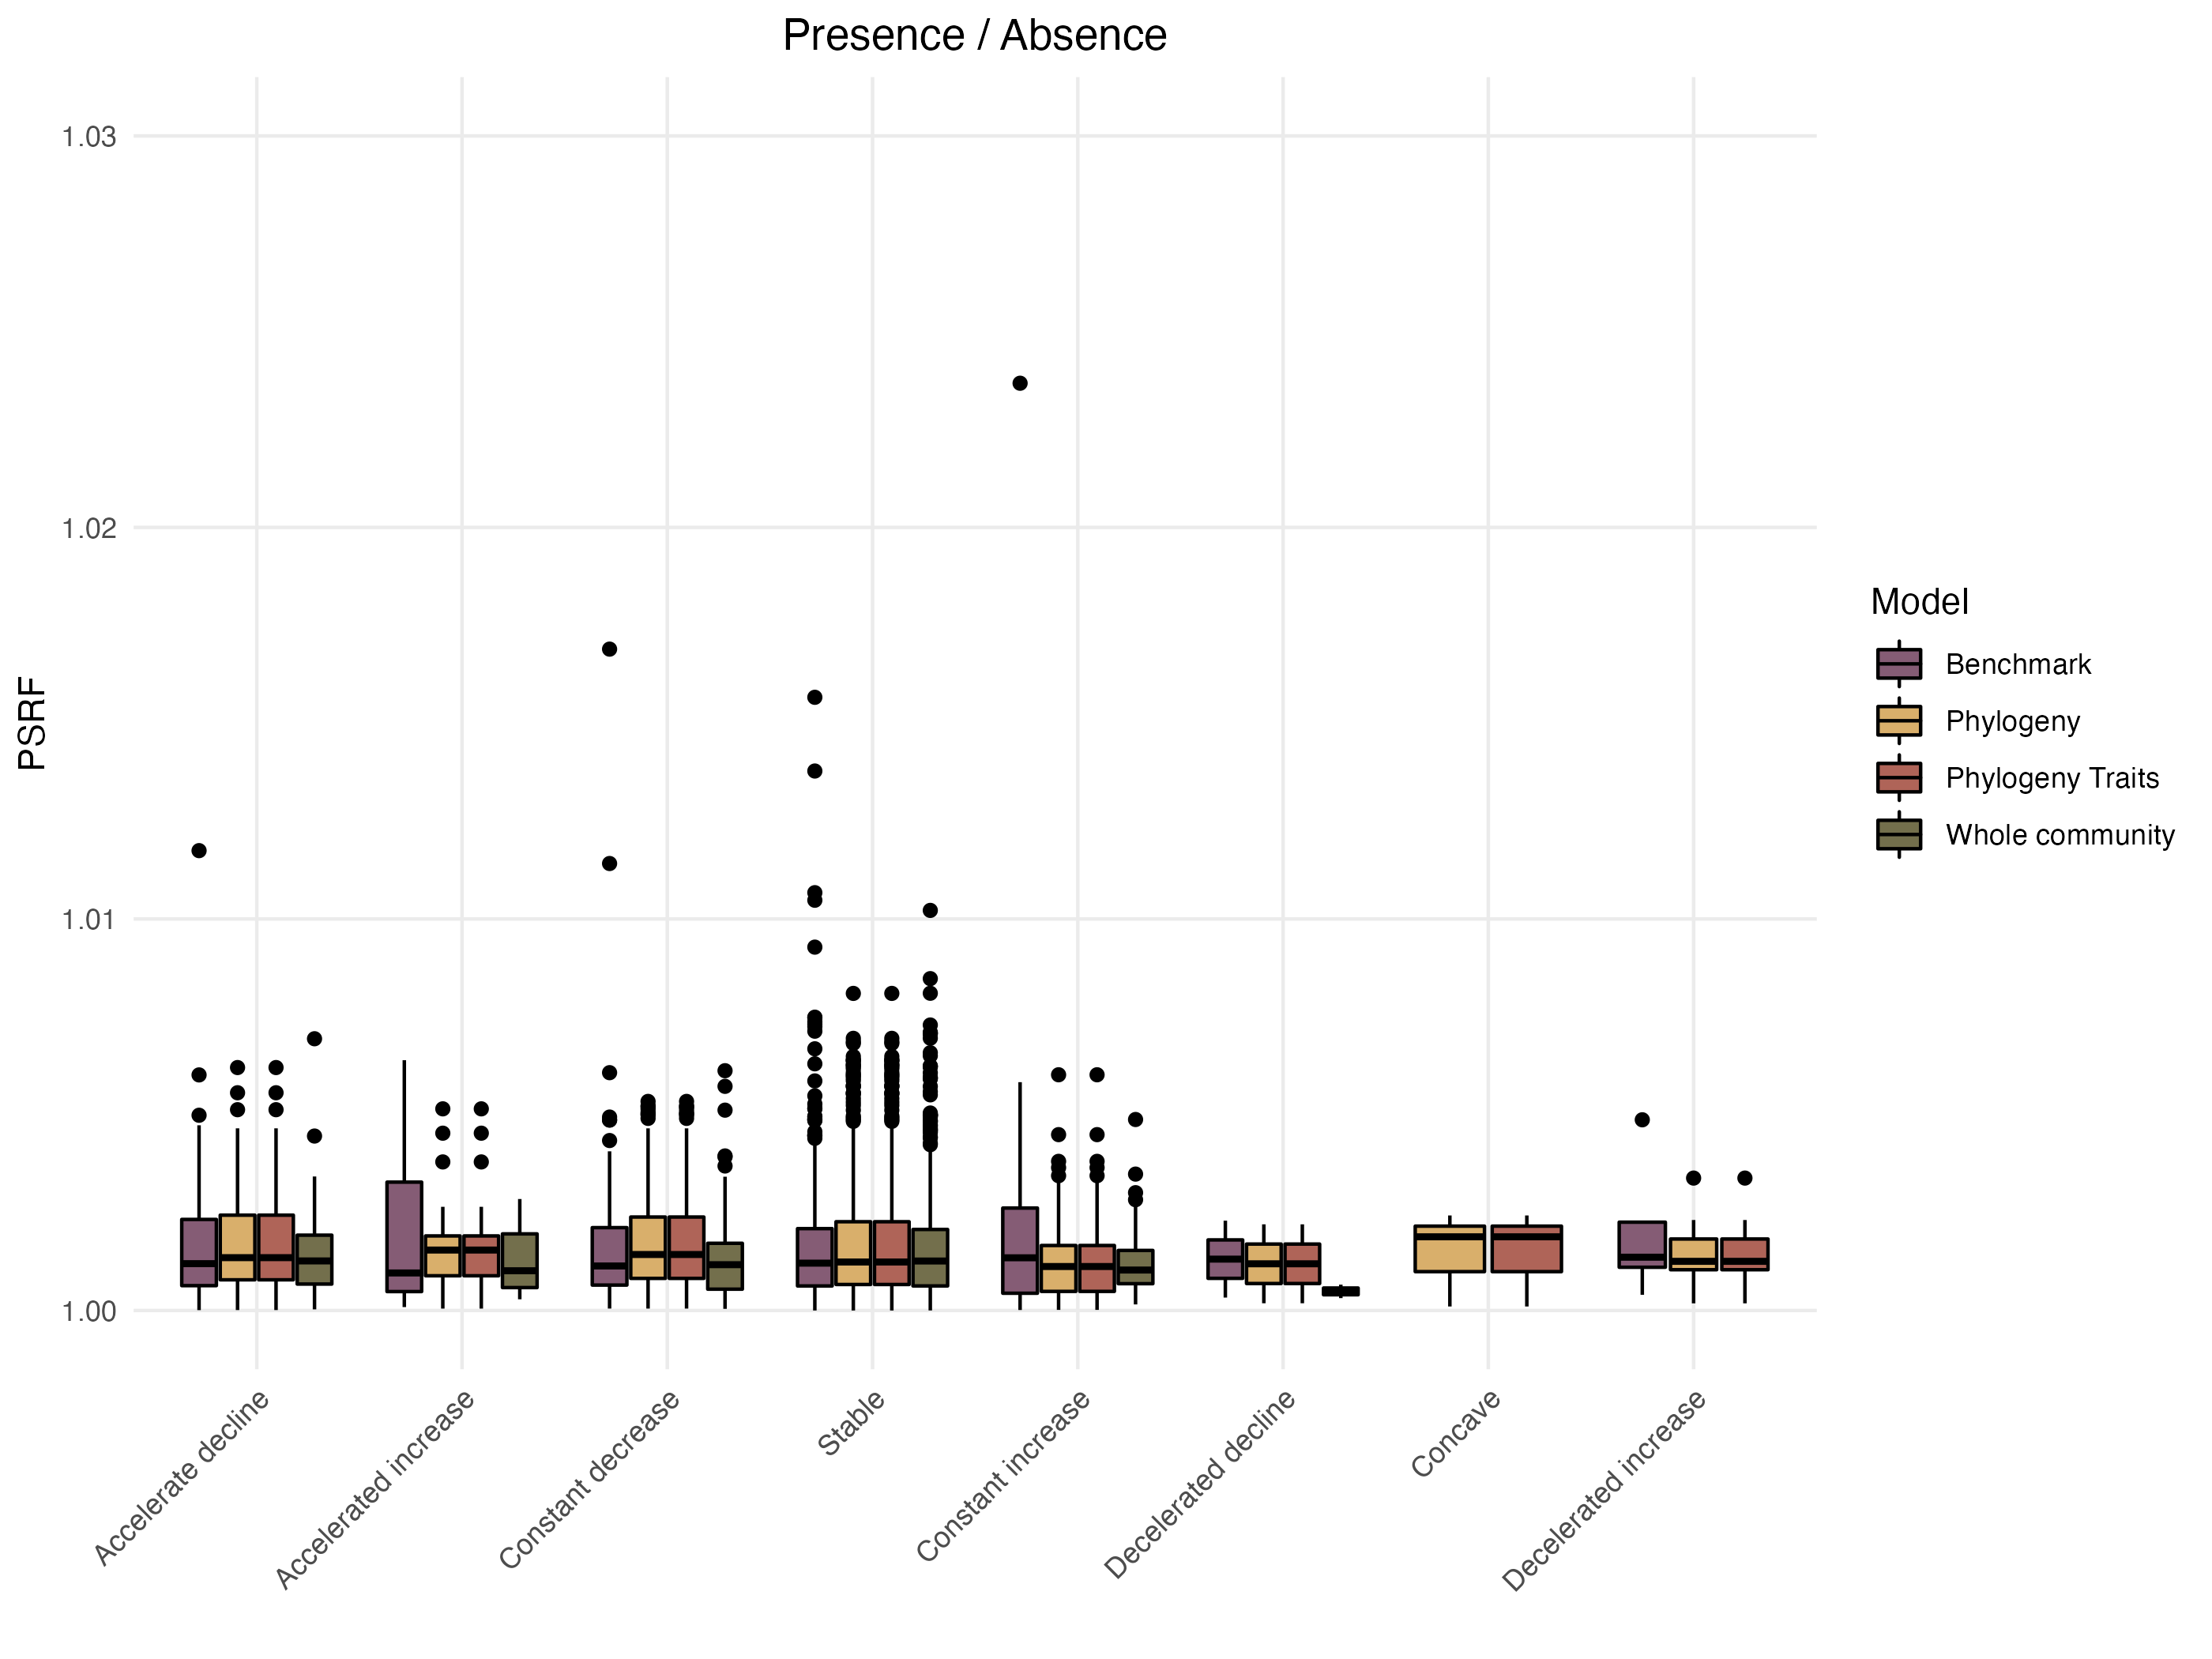
\includegraphics{03-Chapitre1/figures/supplementary/fig_supp16.png}
\caption{Distribution of the Potential scale reduction factors (PSRF) as
a function of the different shapes of the response curves classified
following the methodology proposed by \textcite{Rigal_2020} methods (see
section ``Assessing model performance and interpretability'' section for
more details on the calculation methodology). Results for models fitted
with presence/absence data.}\label{fig:chapt1supp16}
}
\end{figure}

\clearpage

\hypertarget{appendixC-chapter1}{%
\section*{Appendix C - Complementary Results}\label{appendixC-chapter1}}
\addcontentsline{toc}{section}{Appendix C - Complementary Results}

\begin{figure}
\hypertarget{fig:chapt1supp17}{%
\centering
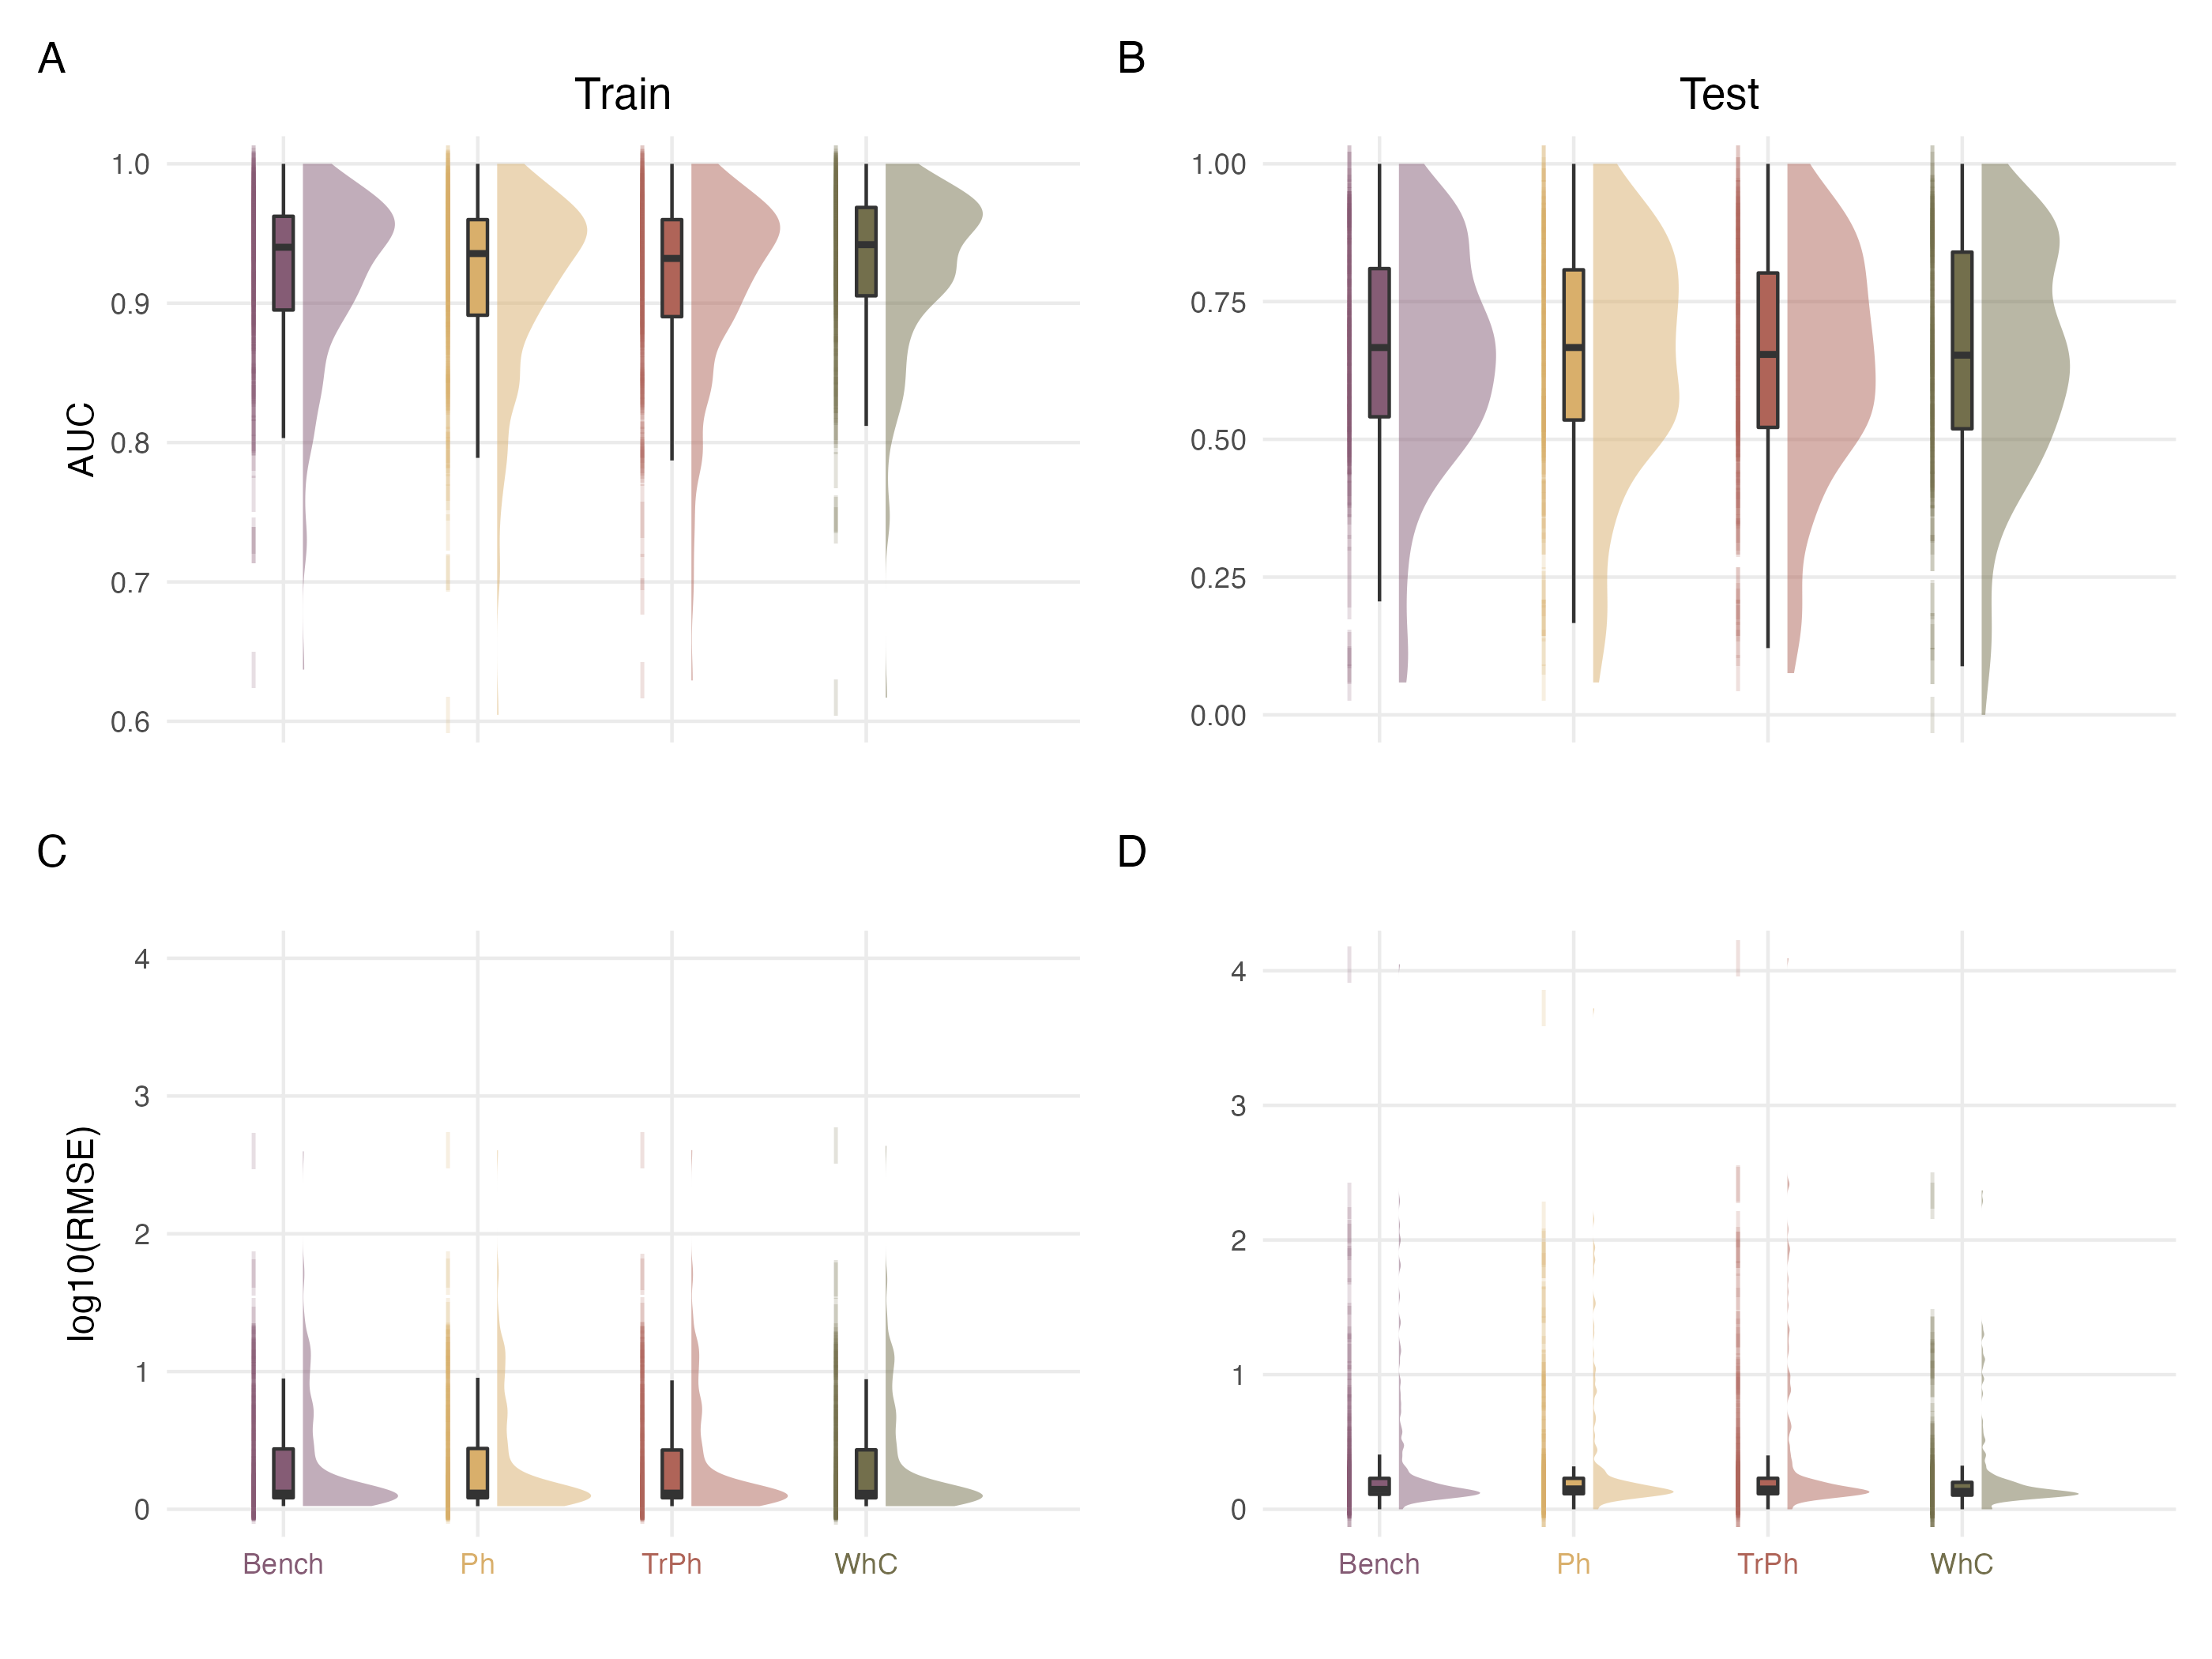
\includegraphics{03-Chapitre1/figures/supplementary/fig_supp17.png}
\caption{Comparison of explanatory (left column; Train set) and
predictive (right column; Test set) performance capacities of the
different model structures fitted on presence/absence (top panels) or
abundance (bottom panels) data}\label{fig:chapt1supp17}
}
\end{figure}

\begin{figure}
\hypertarget{fig:chapt1supp18}{%
\centering
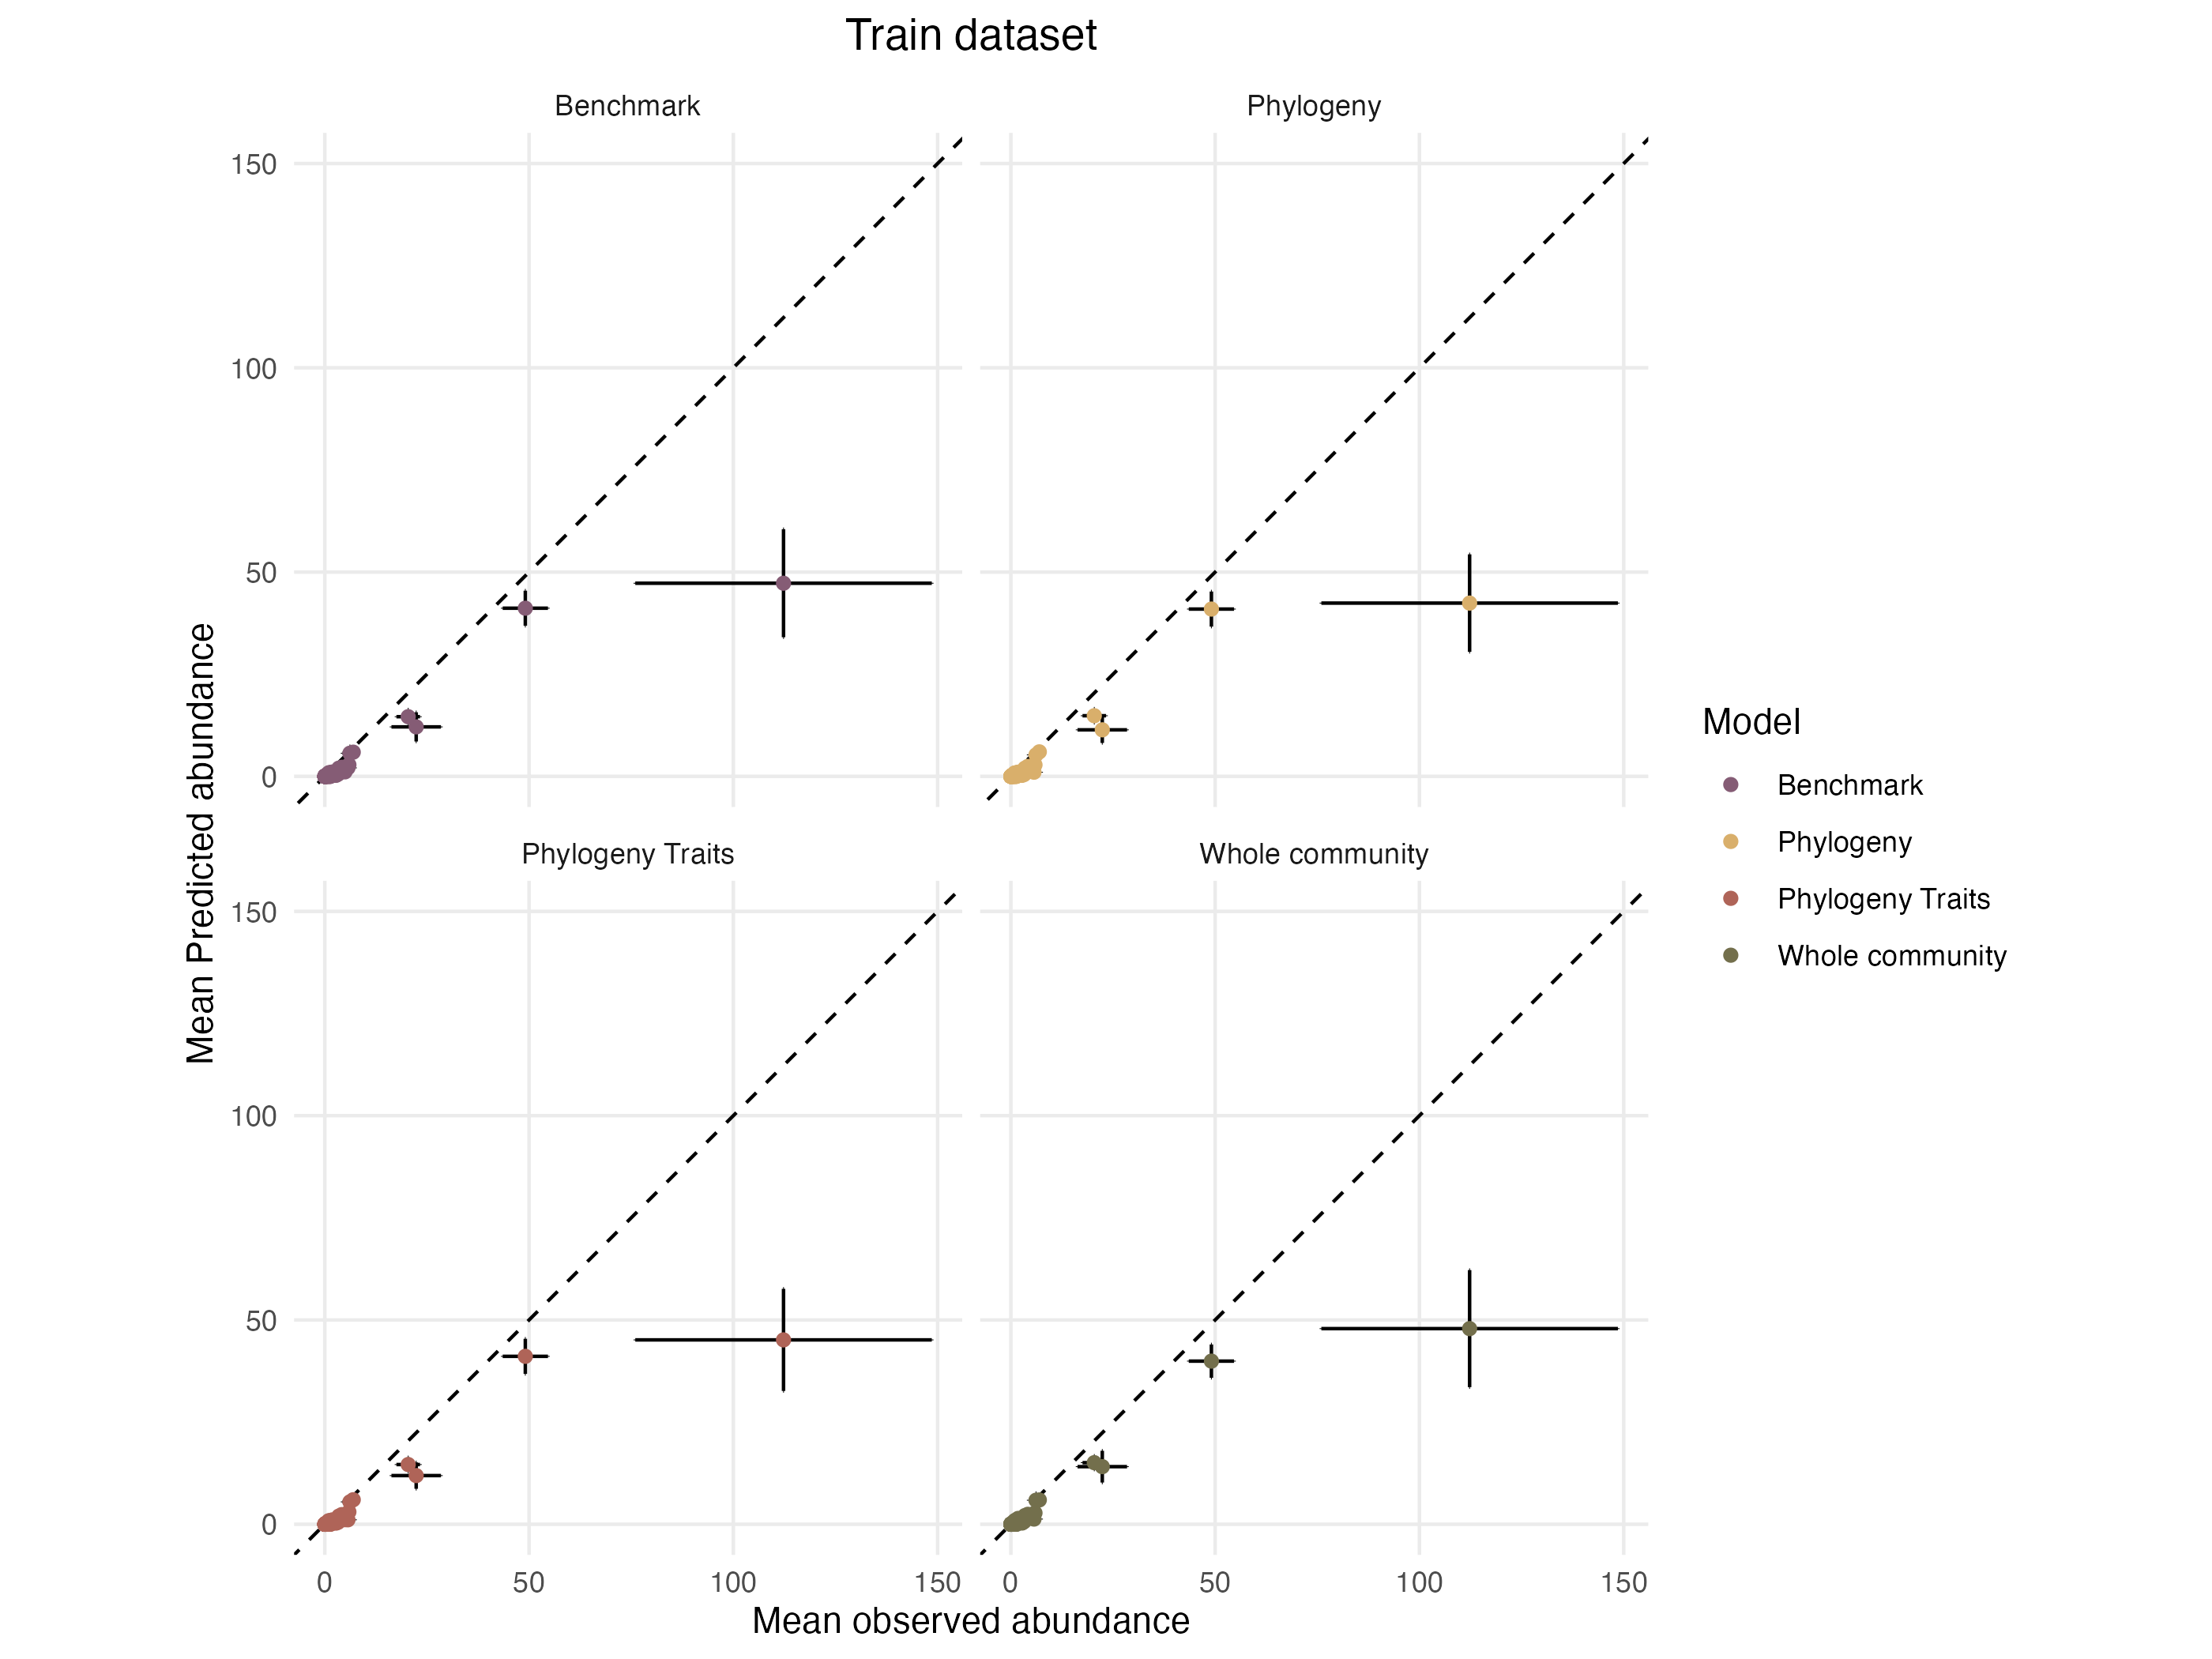
\includegraphics{03-Chapitre1/figures/supplementary/fig_supp18.png}
\caption{Mean predicted abundances as a function of mean observed
abundances in the training dataset. Each species is represented by a
dot, the error bars on each point indicate the standard error around the
mean relatively to each axis.}\label{fig:chapt1supp18}
}
\end{figure}

\begin{figure}
\hypertarget{fig:chapt1supp19}{%
\centering
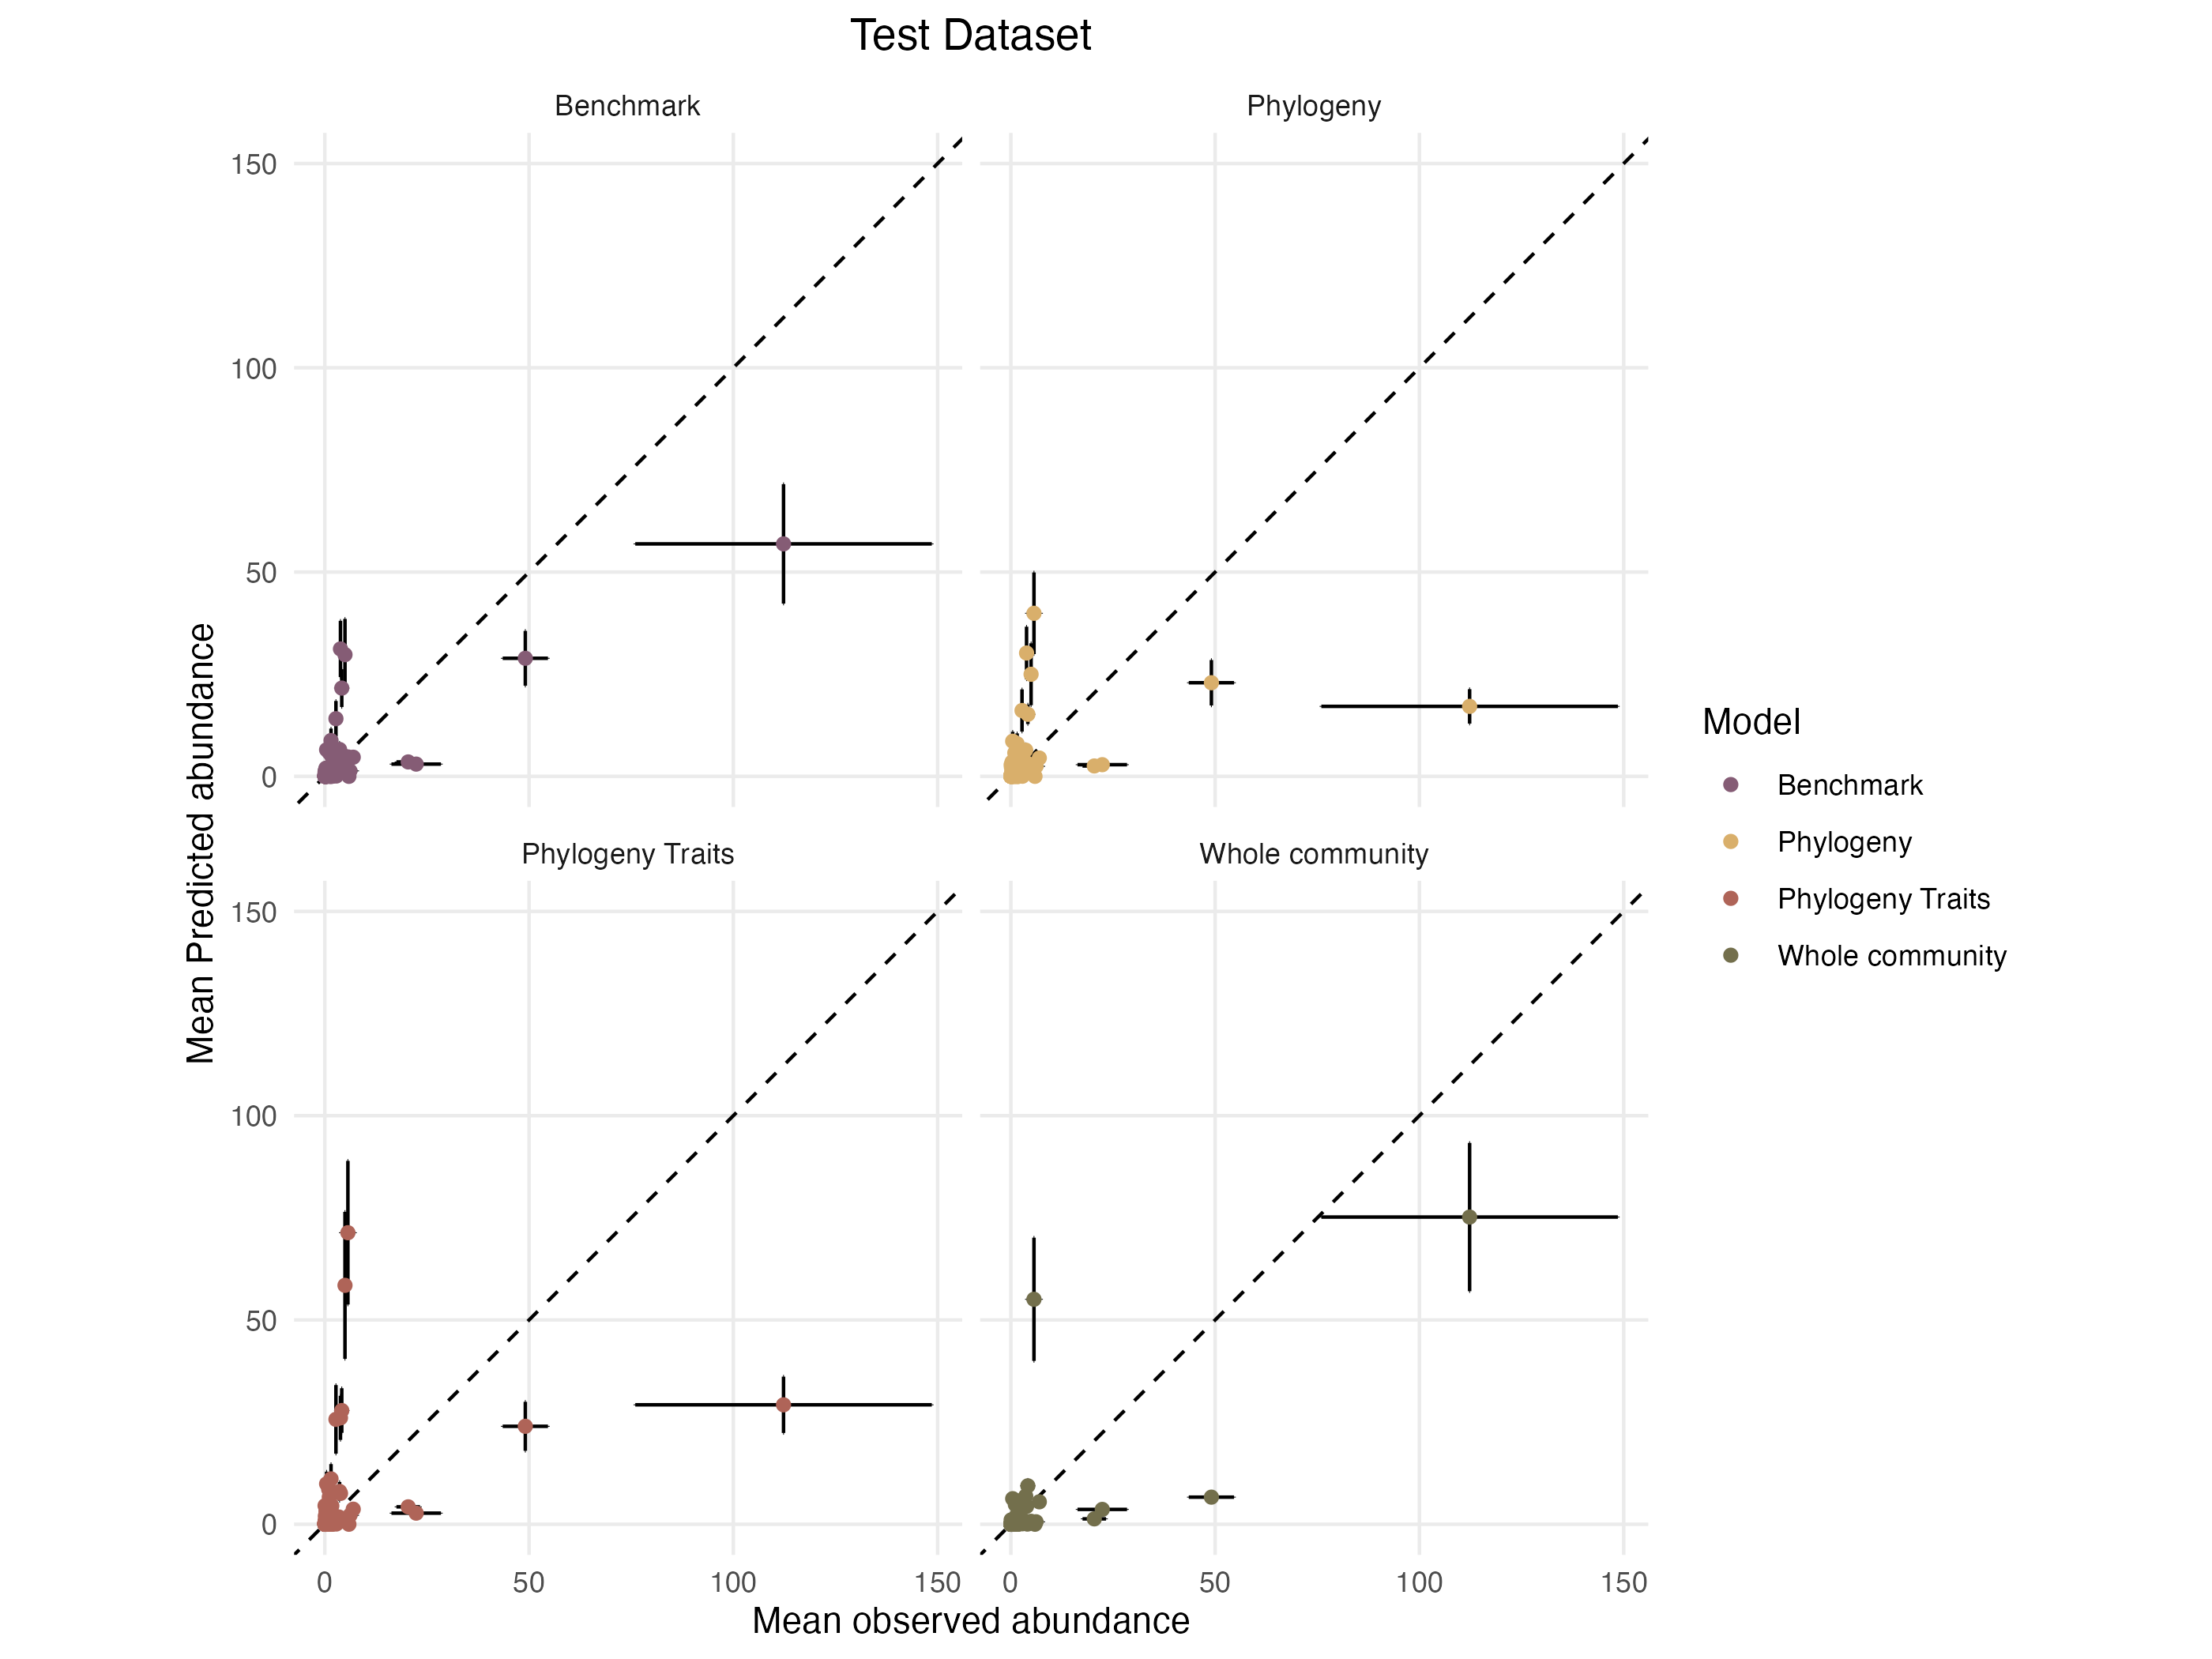
\includegraphics{03-Chapitre1/figures/supplementary/fig_supp19.png}
\caption{Mean predicted abundances as a function of mean observed
abundances in the training dataset. Each species is represented by a
dot, the error bars on each point indicate the standard error around the
mean relatively to each axis.}\label{fig:chapt1supp19}
}
\end{figure}

\begin{figure}
\hypertarget{fig:chapt1supp20}{%
\centering
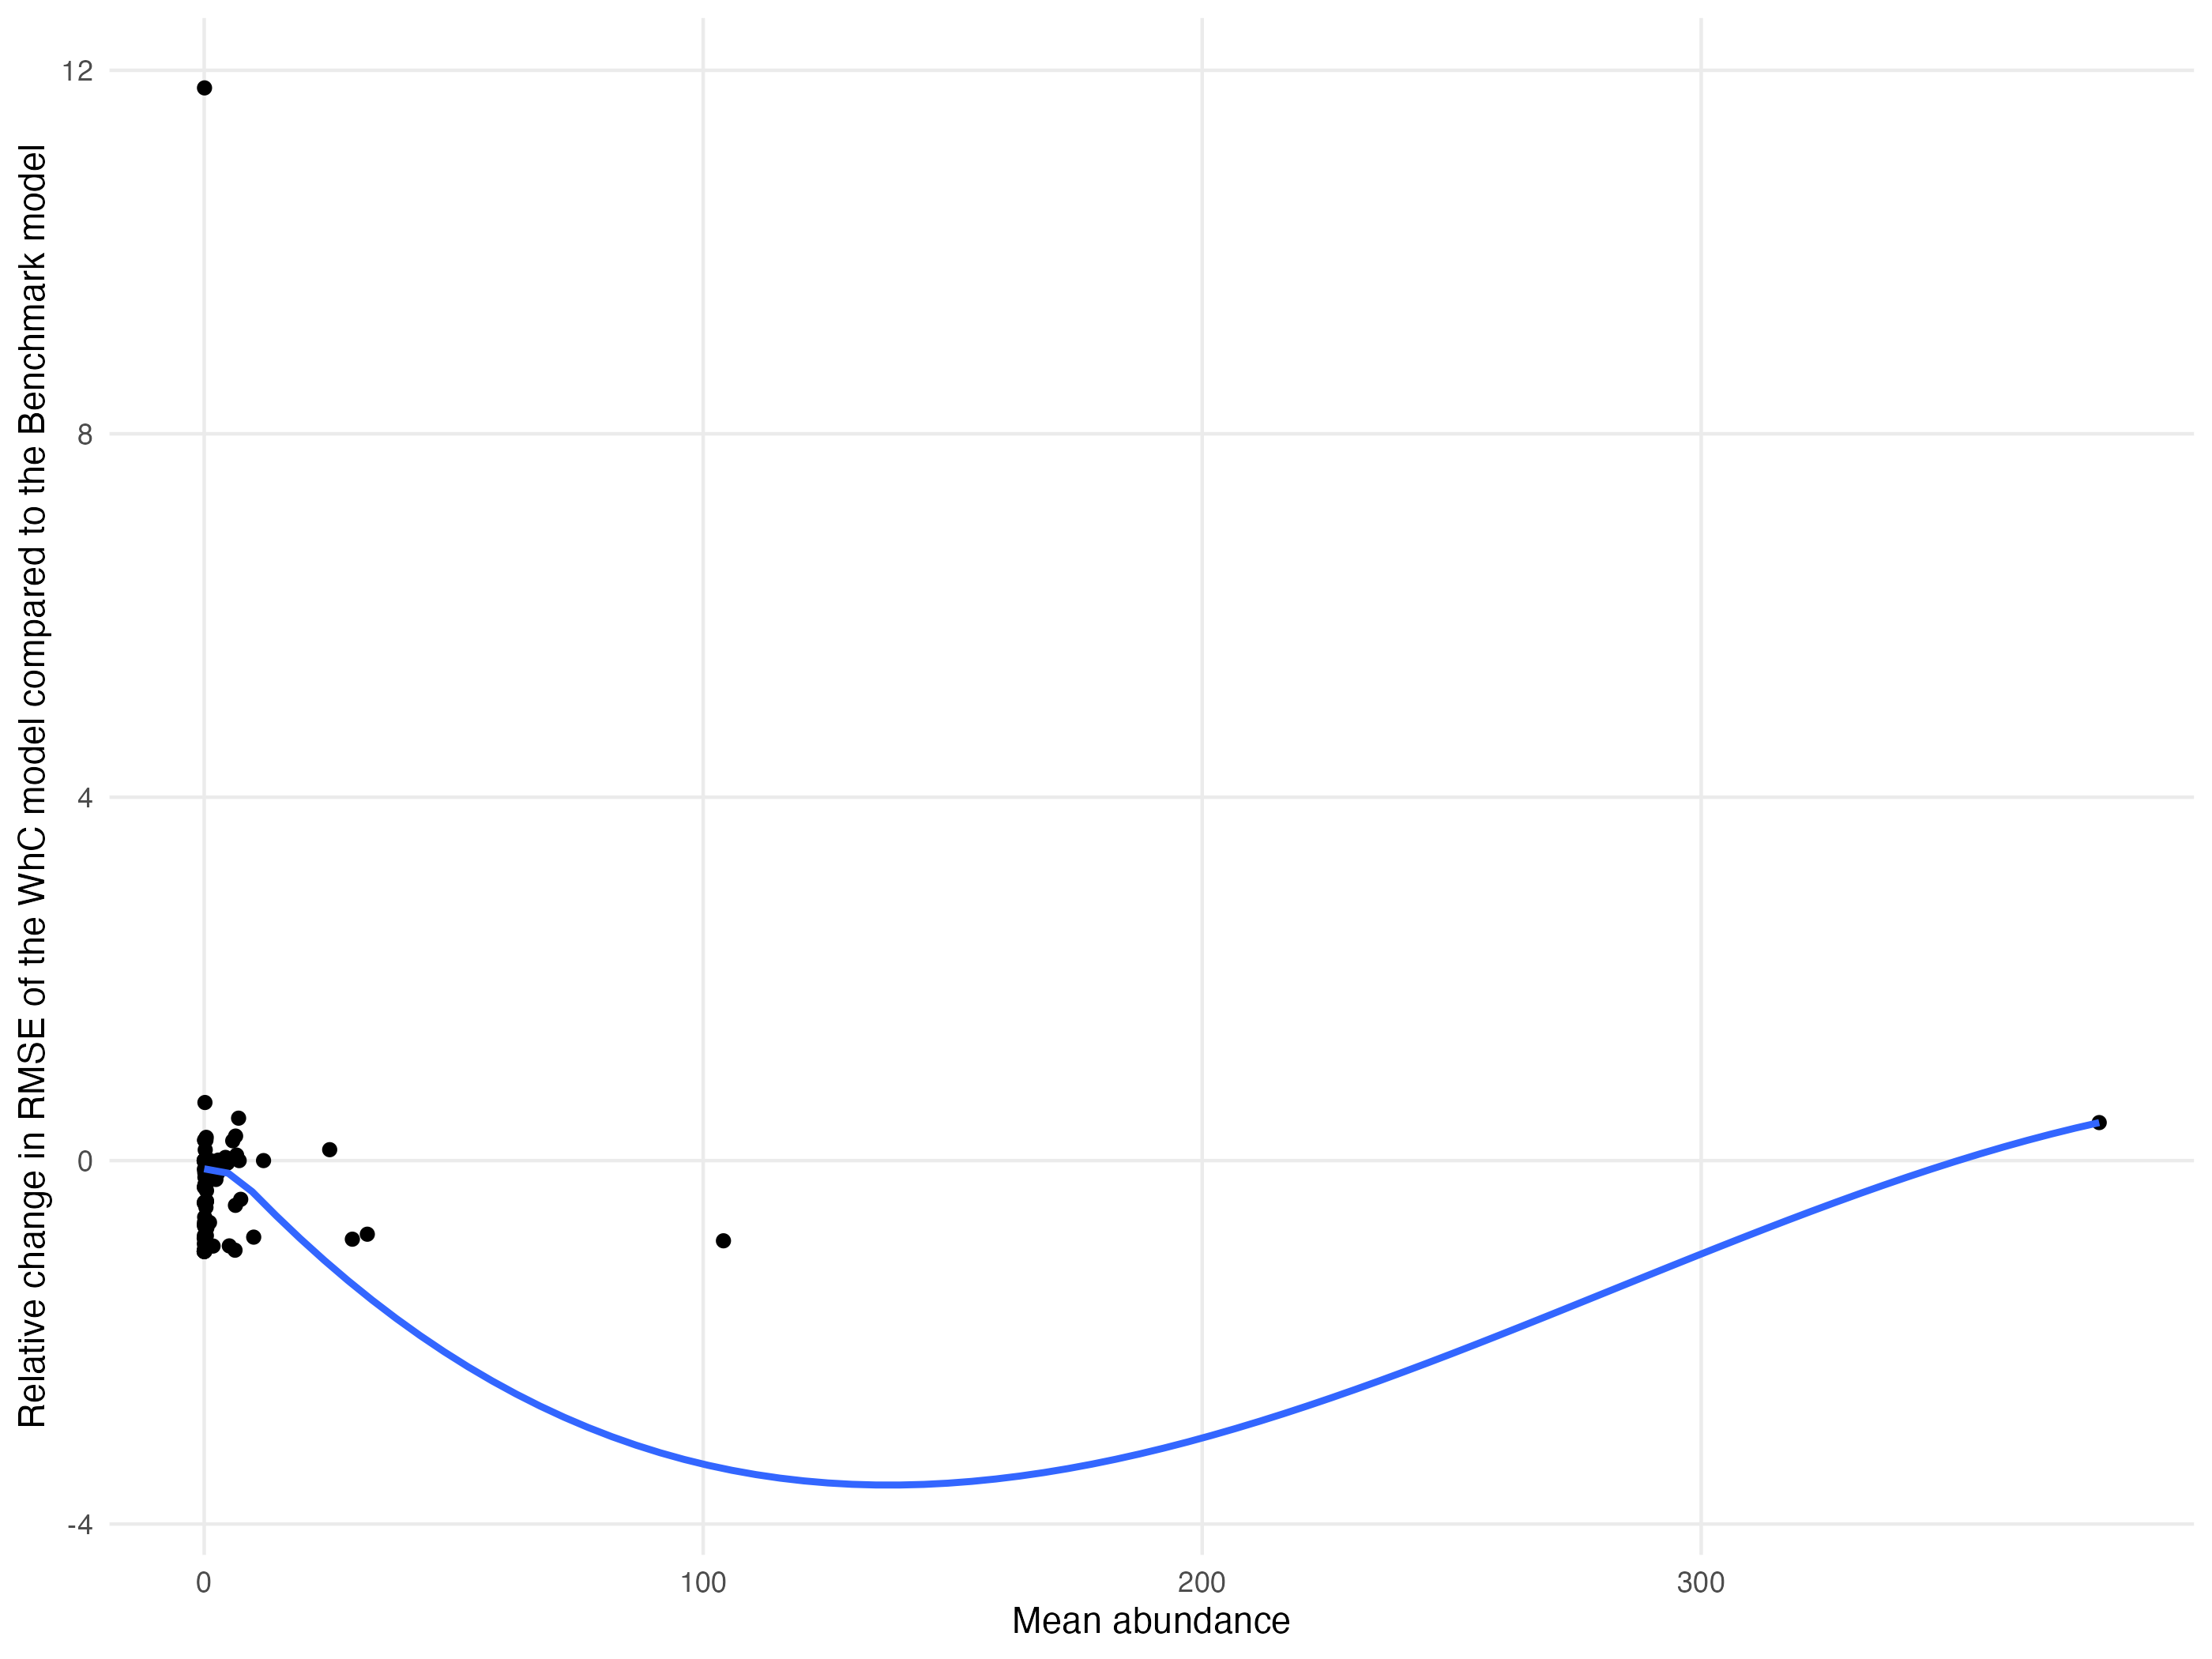
\includegraphics{03-Chapitre1/figures/supplementary/fig_supp20.png}
\caption{Relationship between the relative improvement in RMSE for the
WhC model compared to Bench model and the mean abundance of species in
the training dataset. Each dot represents a species. The blue line
represents a fit obtained from a LOESS
regression.}\label{fig:chapt1supp20}
}
\end{figure}

\begin{figure}
\hypertarget{fig:chapt1supp21}{%
\centering
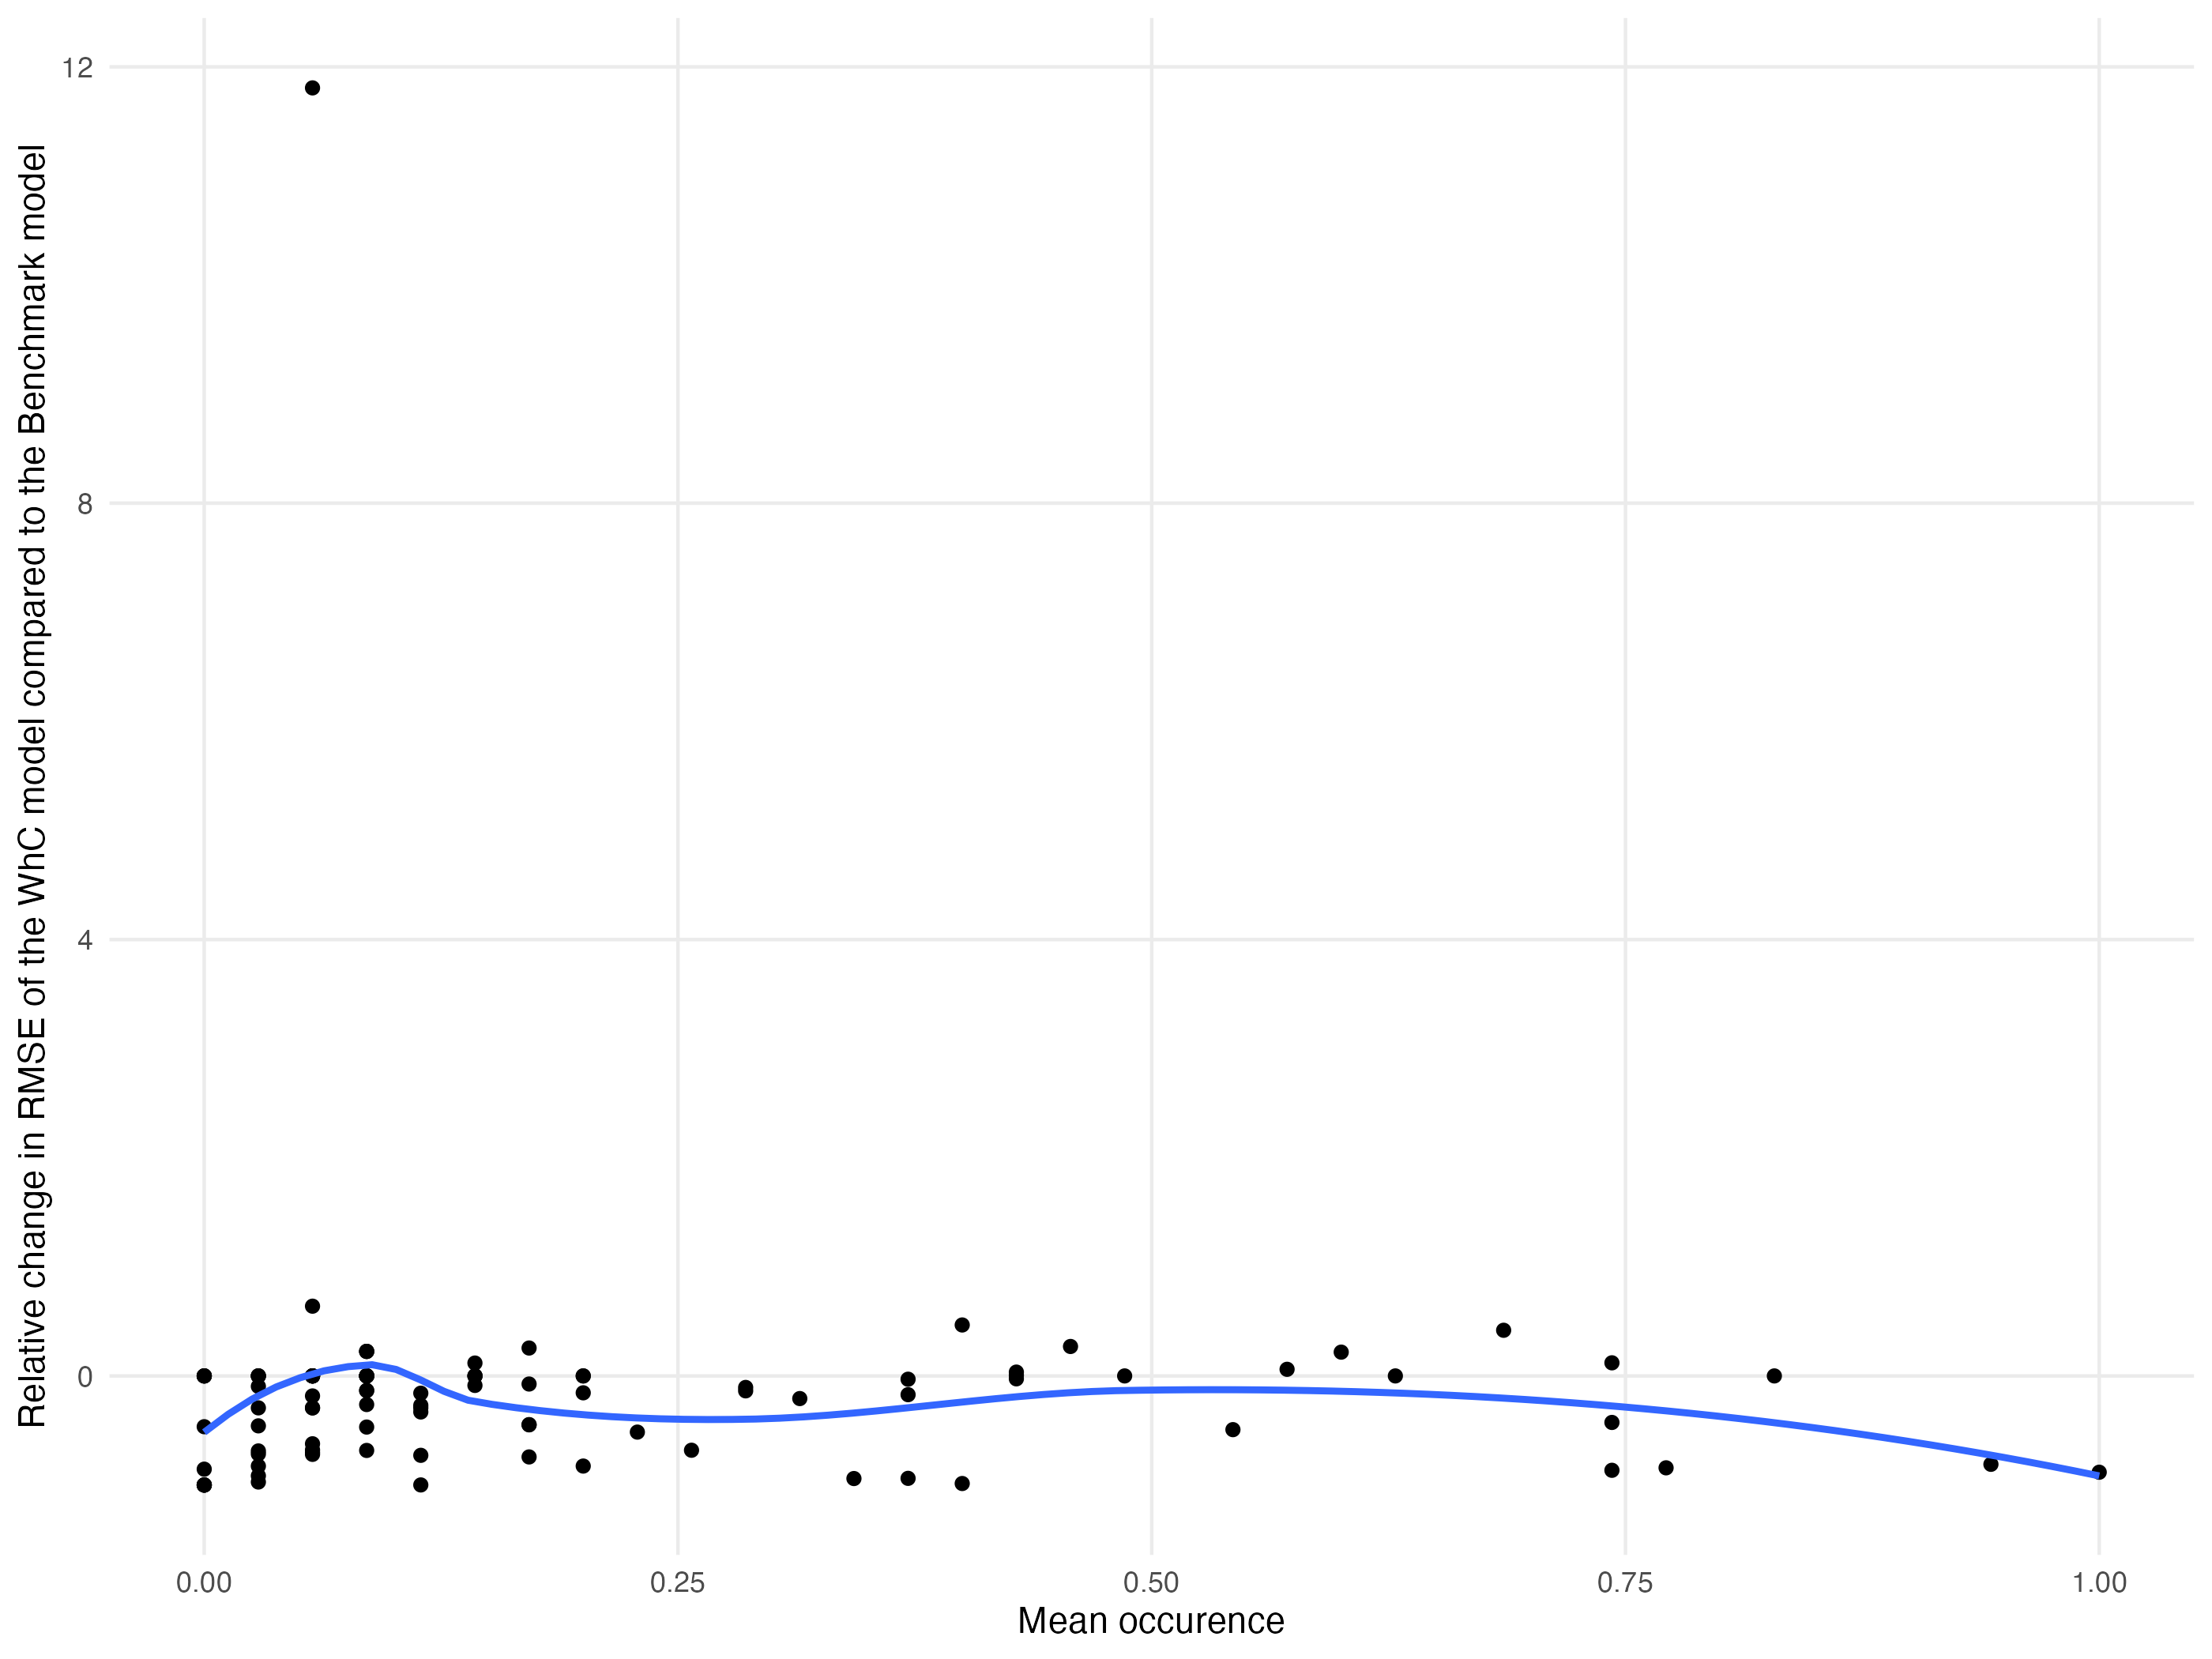
\includegraphics{03-Chapitre1/figures/supplementary/fig_supp21.png}
\caption{Relationship between the relative improvement in RMSE for the
WhC model compared to Bench model and the mean occurrence of species in
the training dataset. Each dot represents a species. The blue line
represents a fit obtained from a LOESS
regression.}\label{fig:chapt1supp21}
}
\end{figure}

\begin{figure}
\hypertarget{fig:fig22}{%
\centering
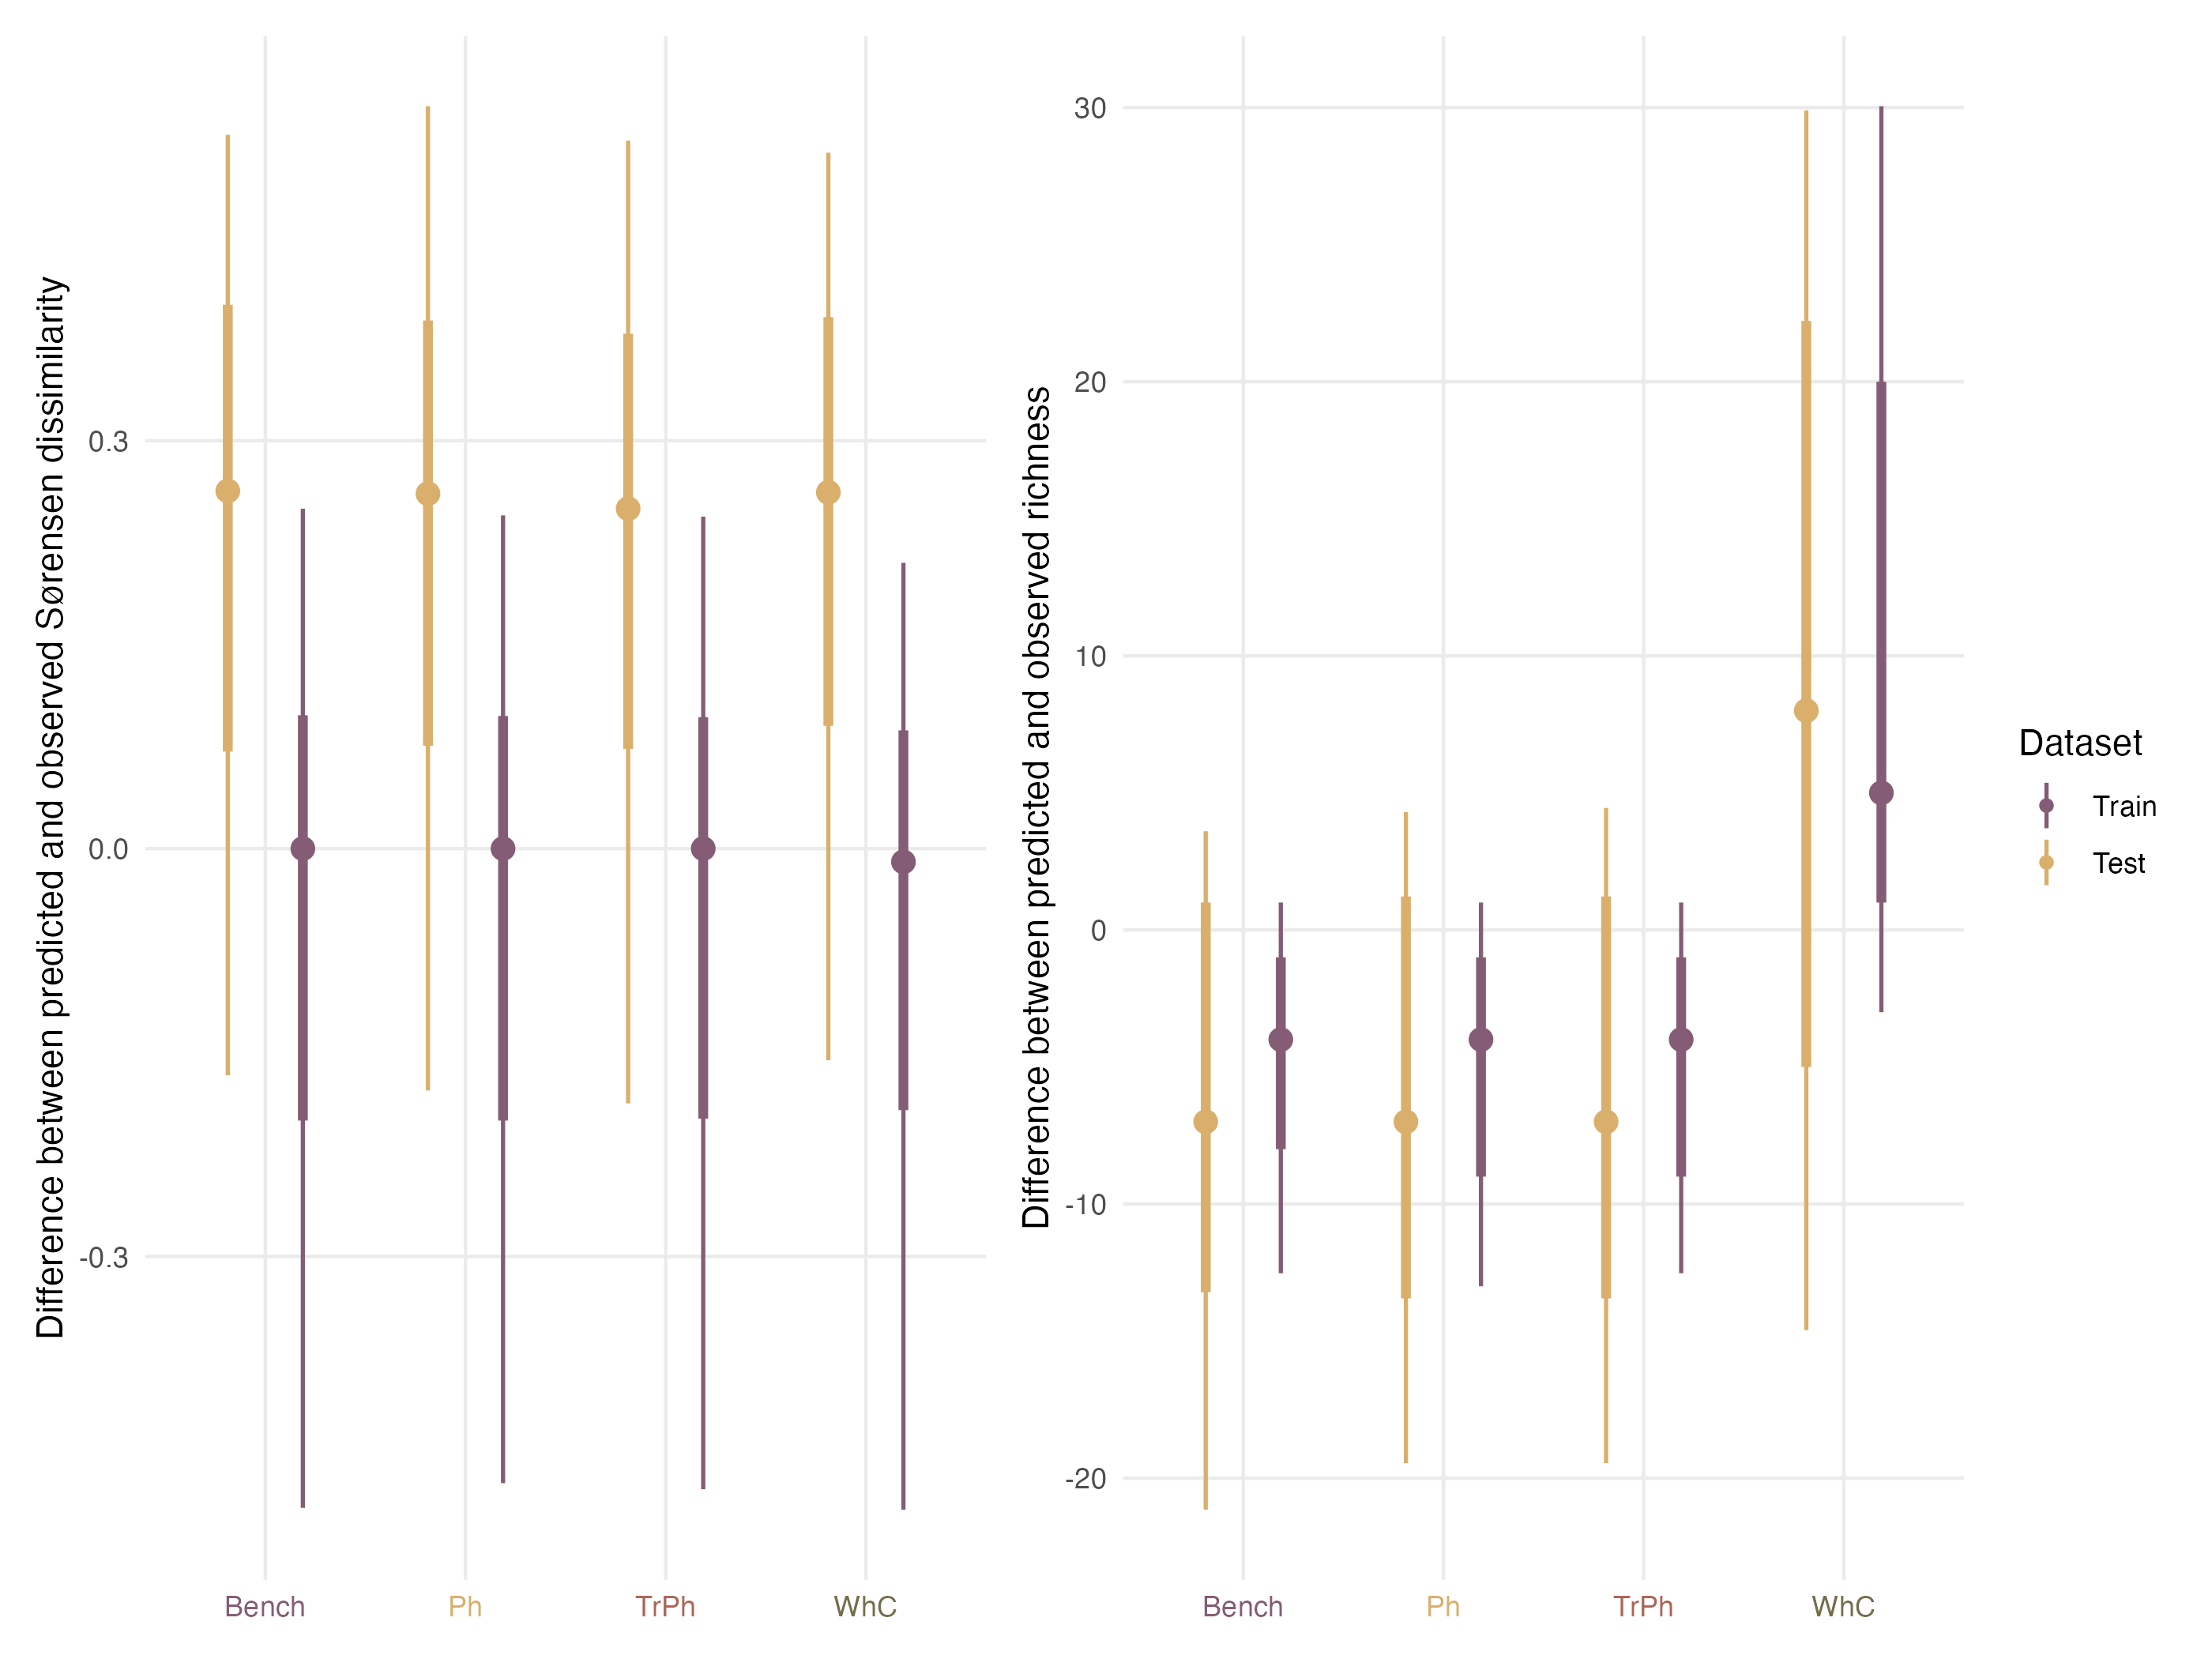
\includegraphics{03-Chapitre1/figures/supplementary/fig_supp22.png}
\caption{Comparison of model performances with regards to their ability
to predict community structures when fitted with presence/absence data
for the train (purple) and test (yellow) dataset. The left column
indicates for each model the difference between the pairwise
dissimilarities computed on the observed assemblages and those computed
on the predicted community. The right column presents the differences in
species richness between the observed and predicted
assemblages.}\label{fig:fig22}
}
\end{figure}

\begin{figure}
\hypertarget{fig:chapt1supp24}{%
\centering
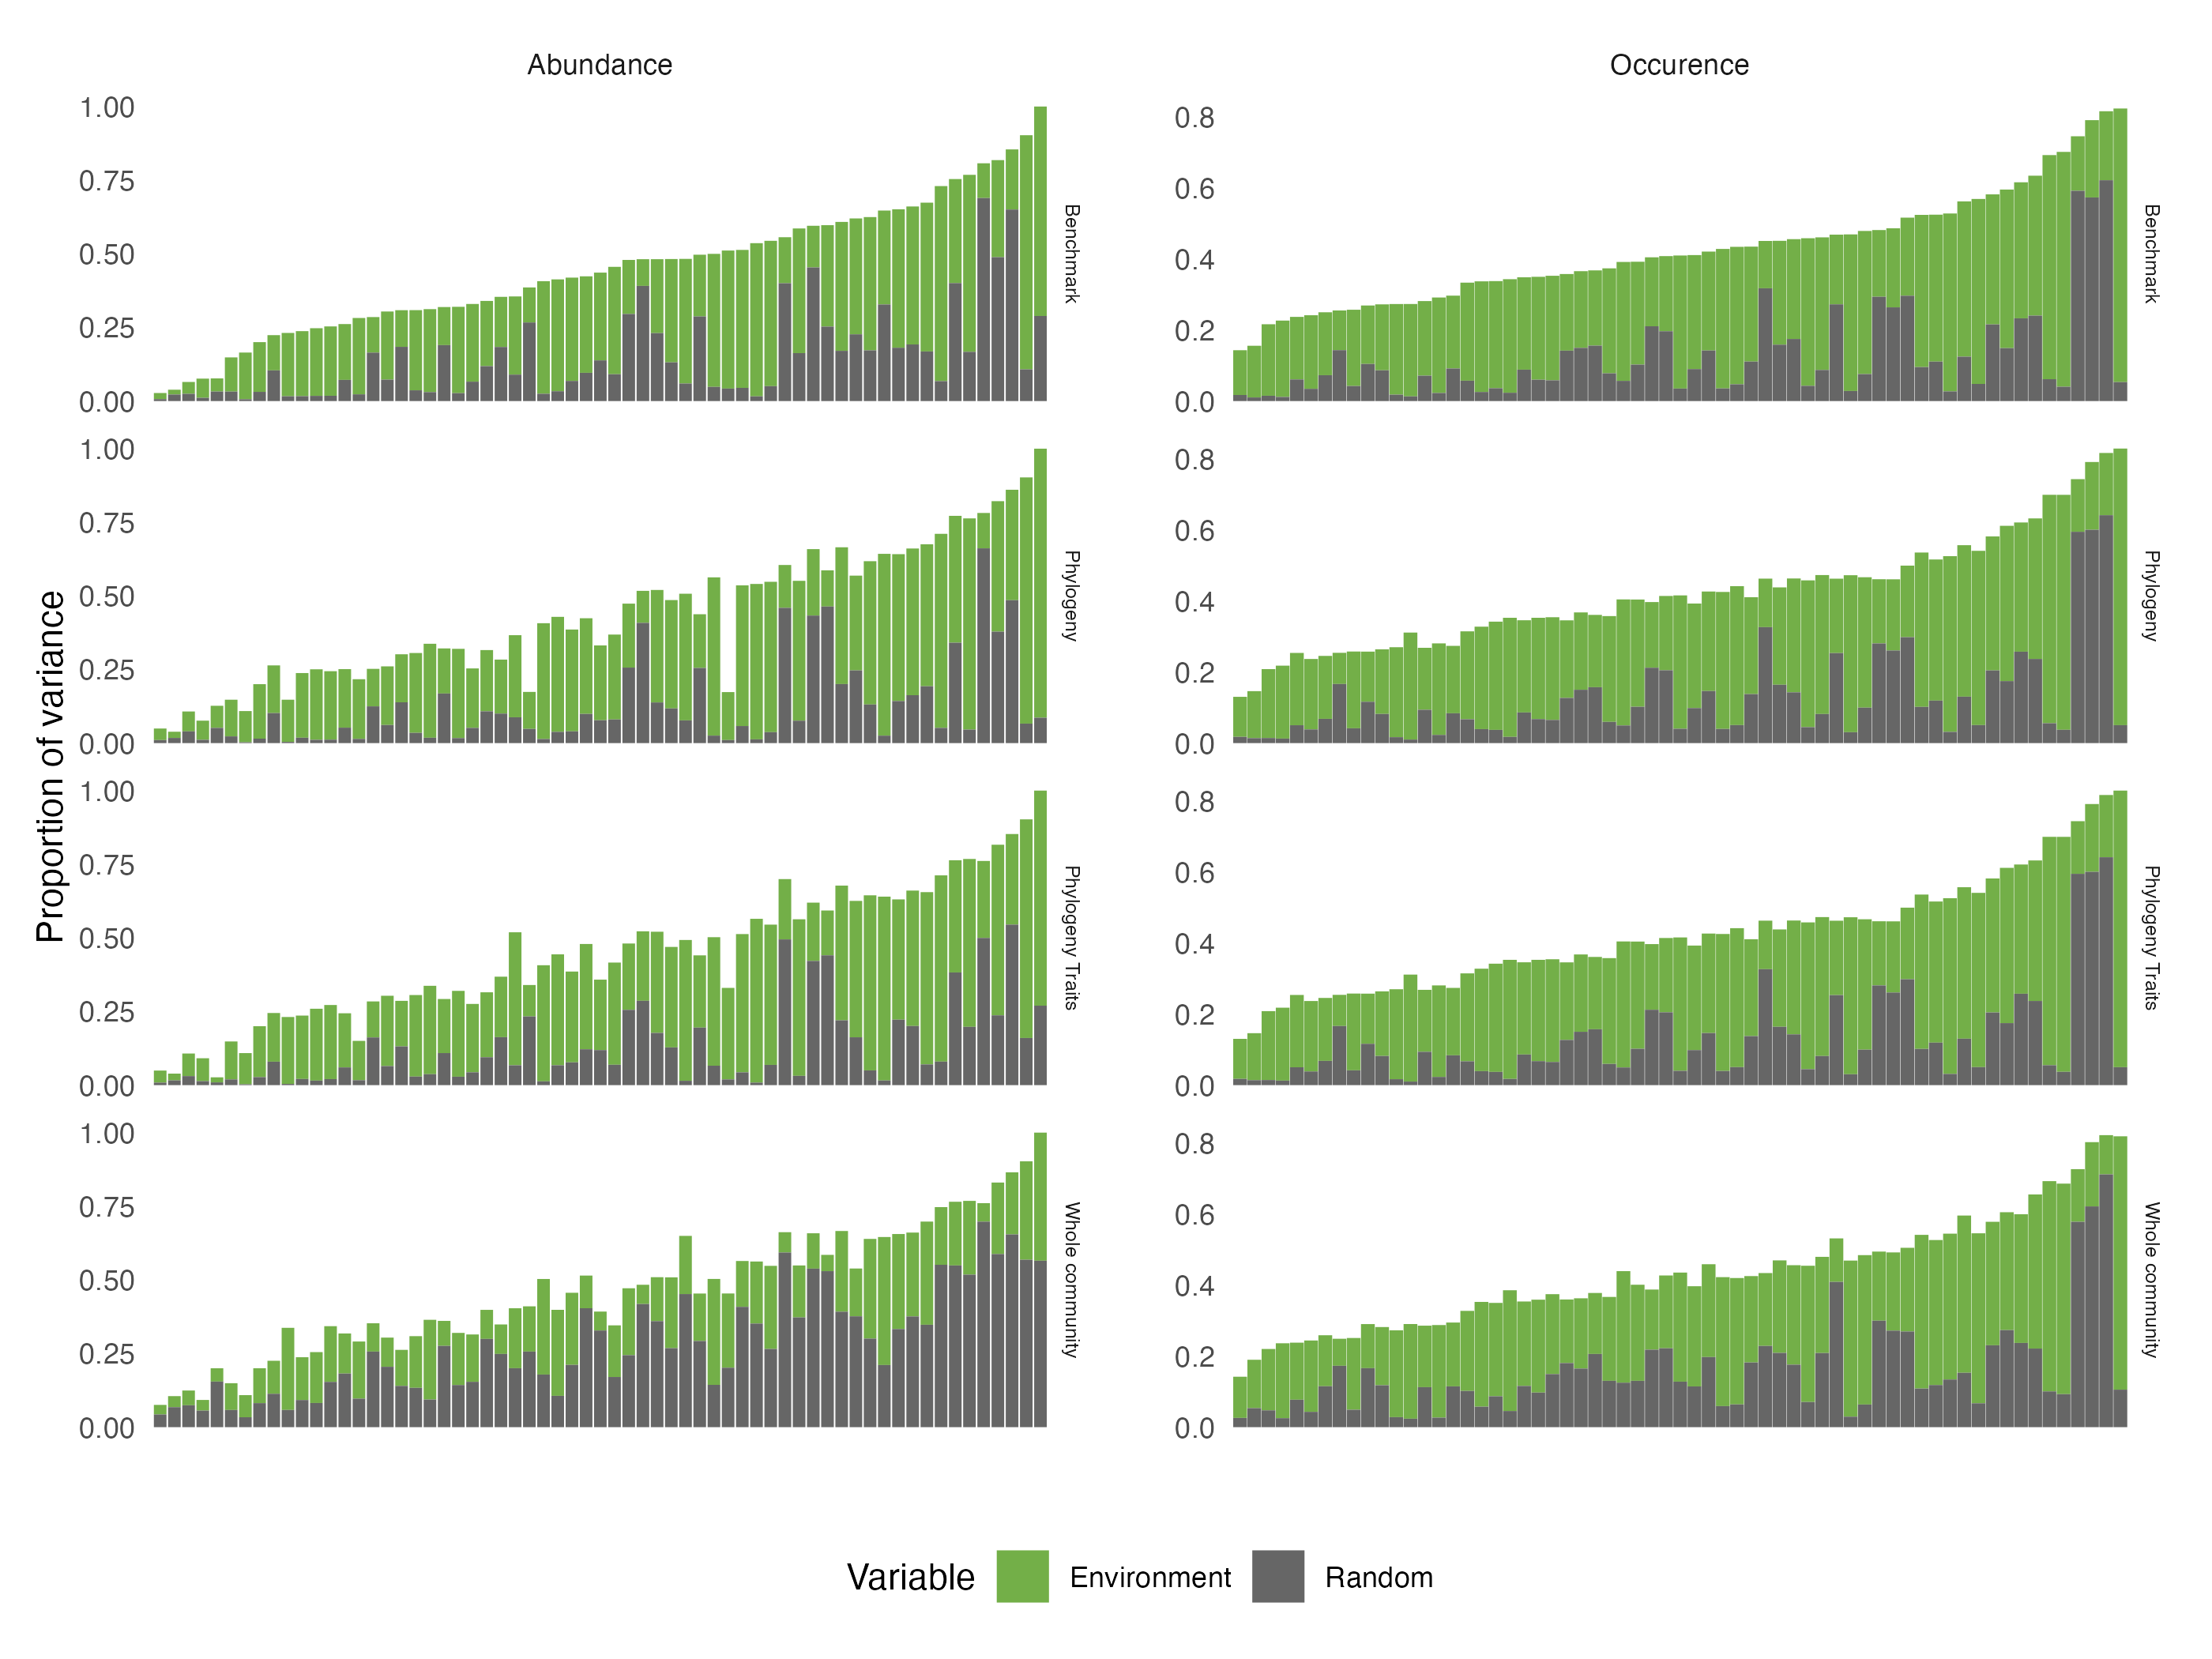
\includegraphics{03-Chapitre1/figures/supplementary/fig_supp24.png}
\caption{Comparison across the four alternative model structures of the
total amount of variance of each species (along the x-axis) that is
explained by (1) the environmental variables (Environment) and (2) the
three random effects (Random). Results are presented for the models
fitted with abundance (left) and presence/absence (right) data. Species
are ordered by increasing order of total variance explained by the
benchmark model.}\label{fig:chapt1supp24}
}
\end{figure}

\begin{figure}
\hypertarget{fig:chapt1supp23}{%
\centering
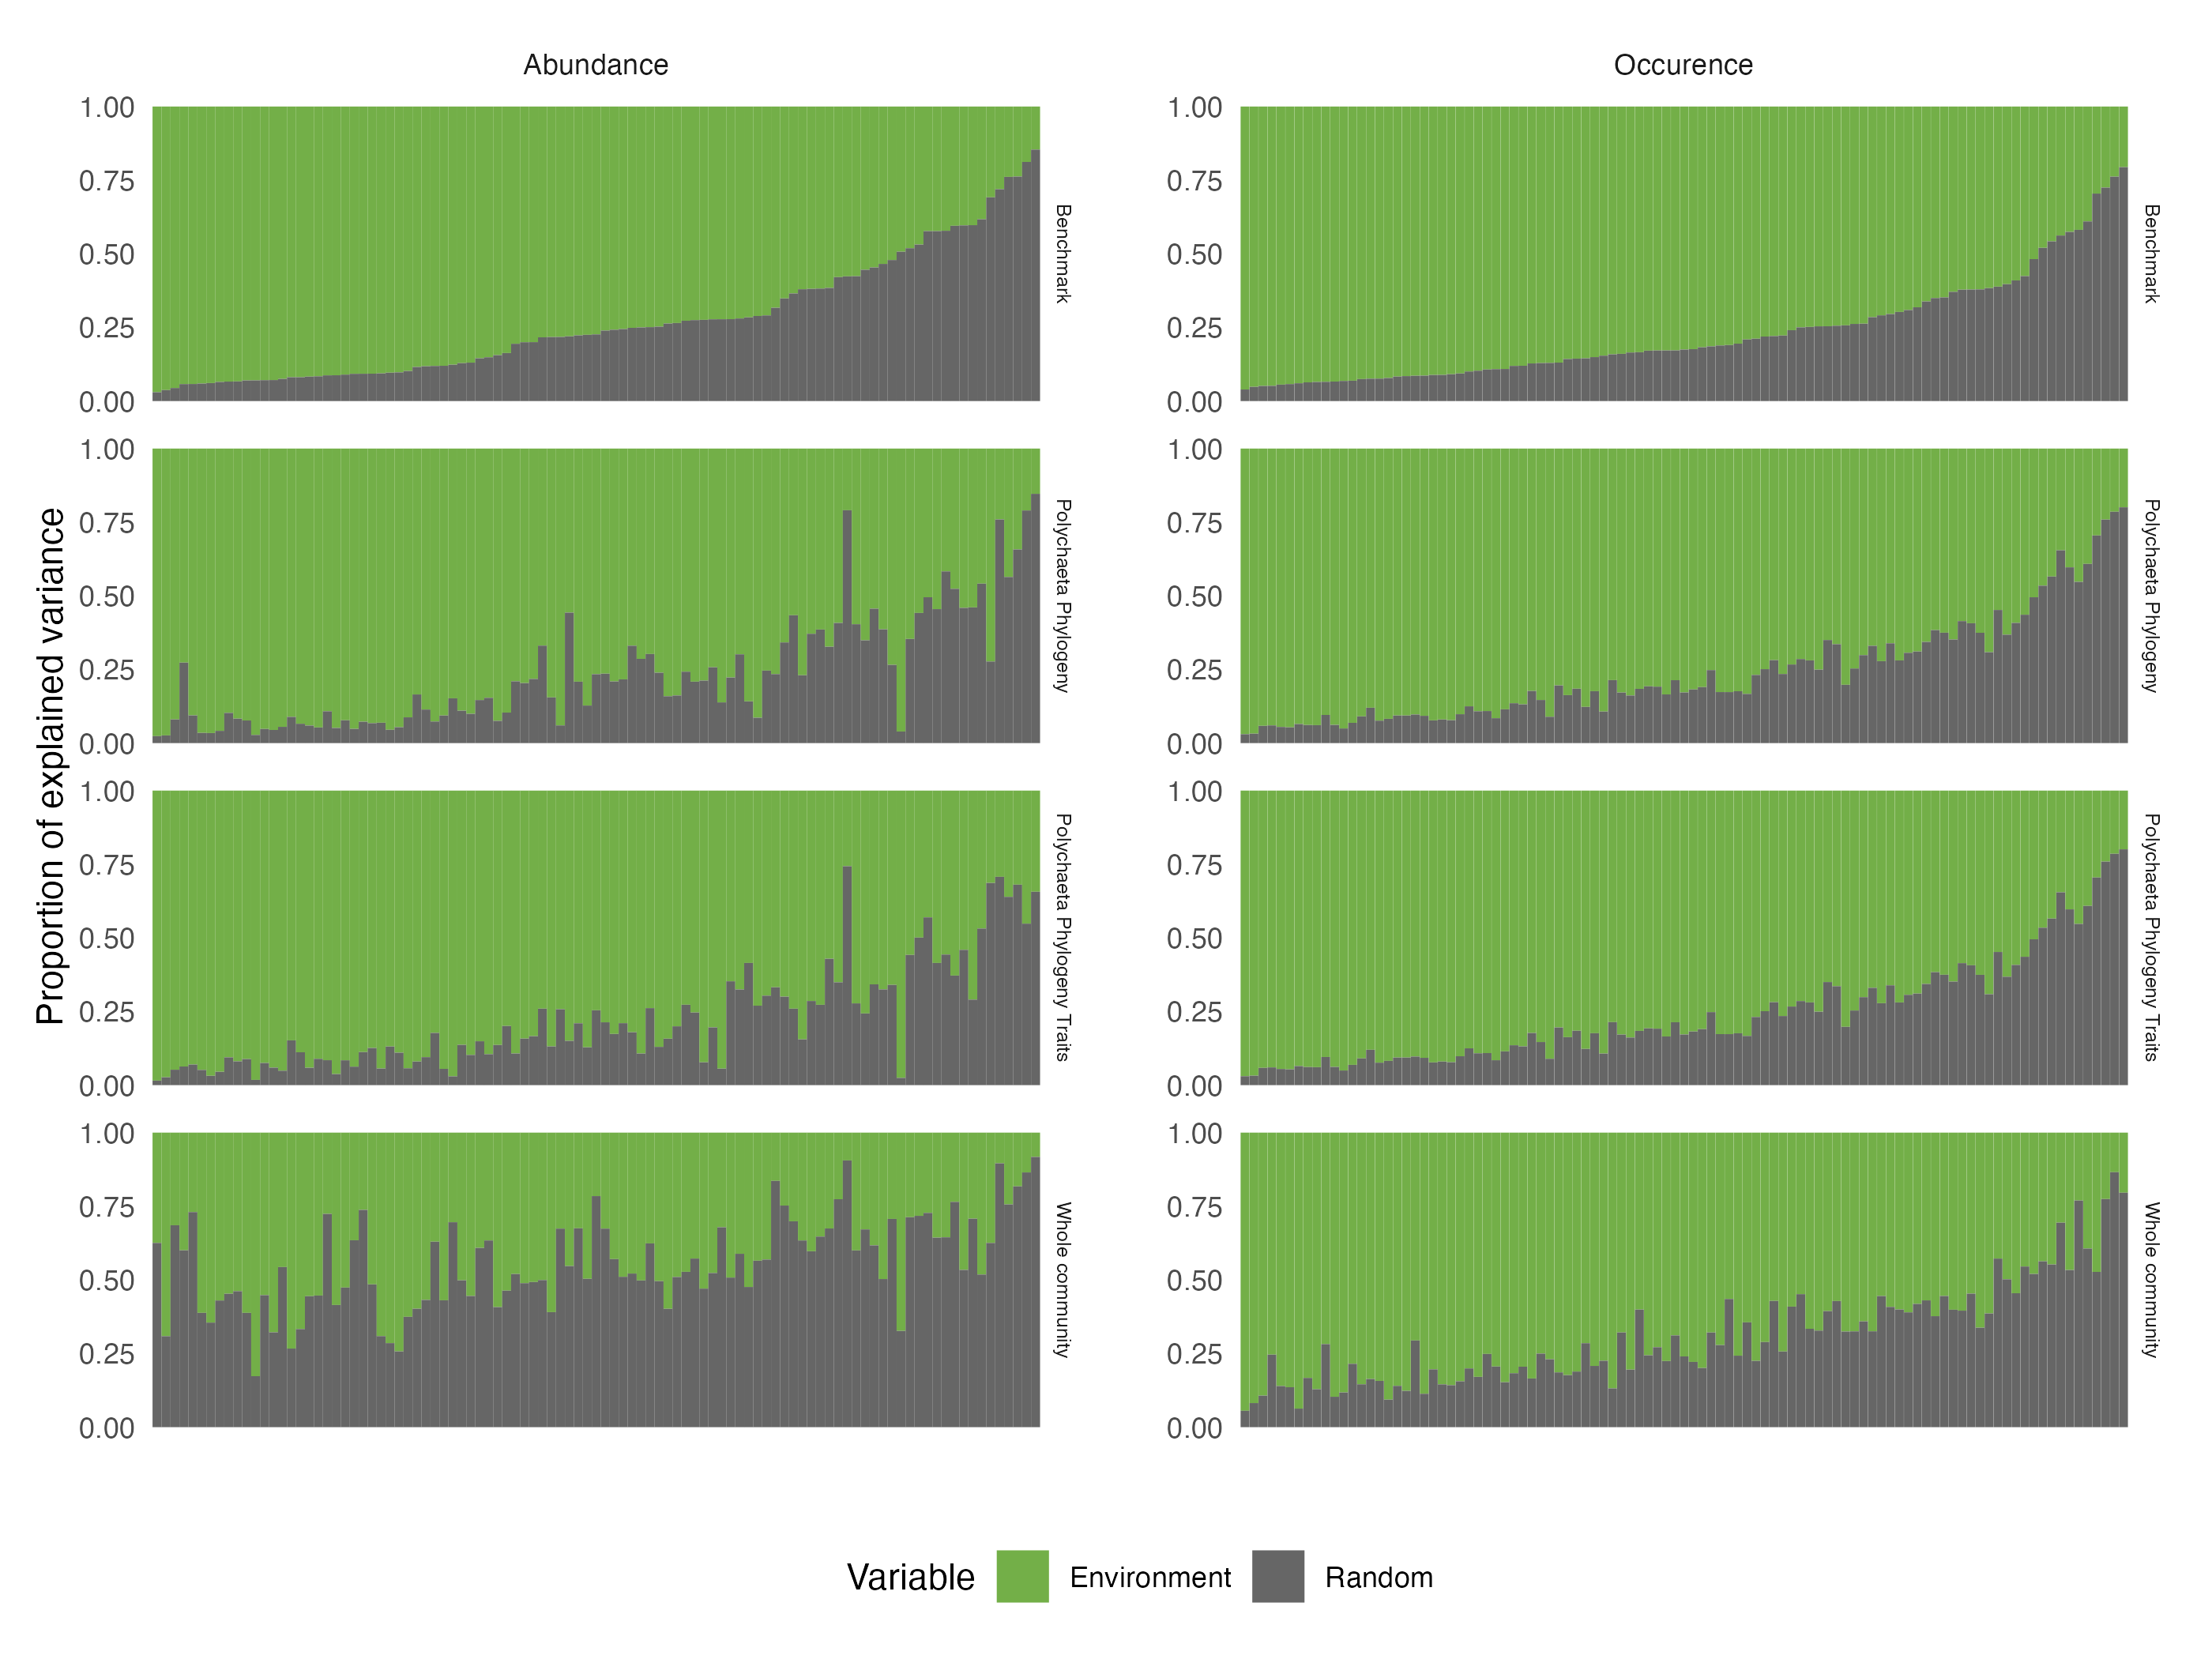
\includegraphics{03-Chapitre1/figures/supplementary/fig_supp23.png}
\caption{Comparison across the four alternative model structures of the
fraction of variance of each species (along the x-axis) that is
explained by (1) the environmental variables (Environment) and (2) the
three random effects (Random). Results are presented for the models
fitted with abundance (left) and presence/absence (right) data. Species
are ordered by decreasing order of variance explained by the environment
for the benchmark model.}\label{fig:chapt1supp23}
}
\end{figure}

\begin{figure}
\hypertarget{fig:chapt1supp26}{%
\centering
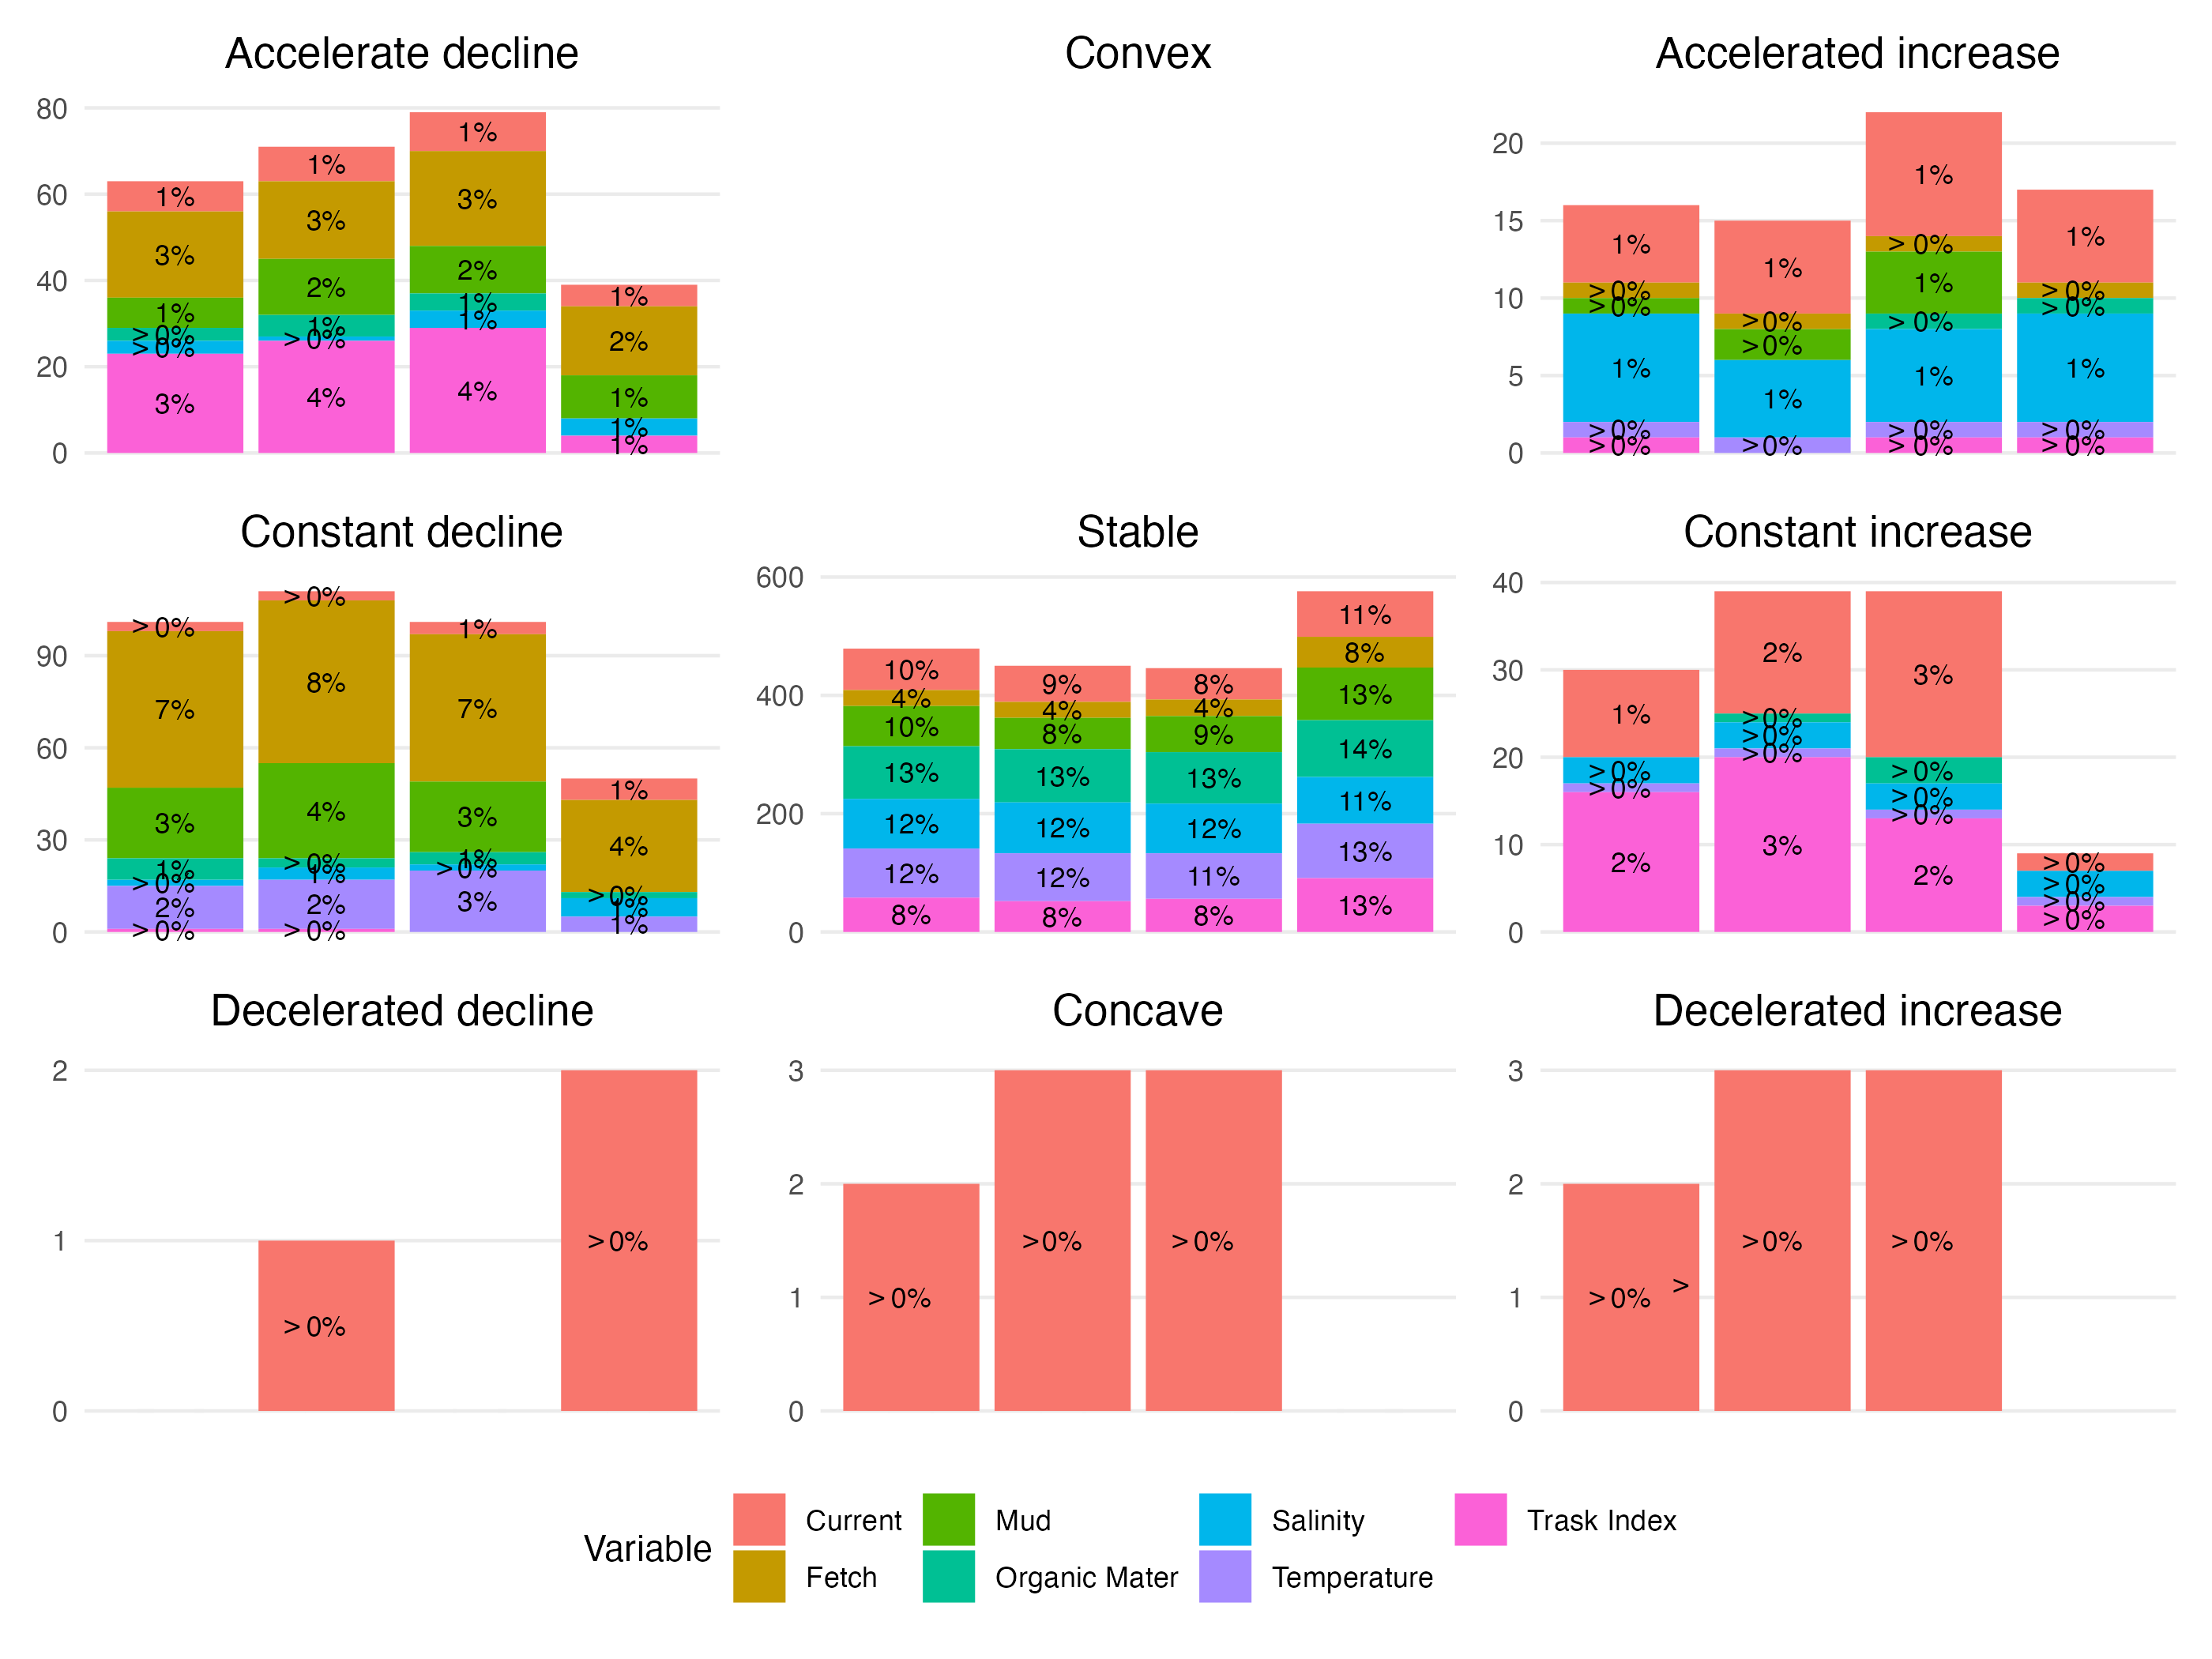
\includegraphics{03-Chapitre1/figures/supplementary/fig_supp26.png}
\caption{Same figure as Fig. 4 in the main text for models fitted on
abundance data. Number (y-axis) and proportion (indicated above
individual bars, rounded to the nearest integer) of response curves
(i.e.~one for each species-predictor combination) according to the
nomenclature (nine shapes highlighted by the black curve in each panel)
defined by \textcite{Rigal_2020}. Results are presented for different
model structures: from left to right the Benchmark (Bench), the
phylogeny (Ph), the traits \& phylogeny (TrPh), and the whole community
(WhC) models. Each bar is coloured by the relative contribution of each
environmental covariate to this particular shape. For illustrative
purposes, note that the scale of variation on the y-axis differs across
panels.}\label{fig:chapt1supp26}
}
\end{figure}

\begin{figure}
\hypertarget{fig:chapt1supp25}{%
\centering
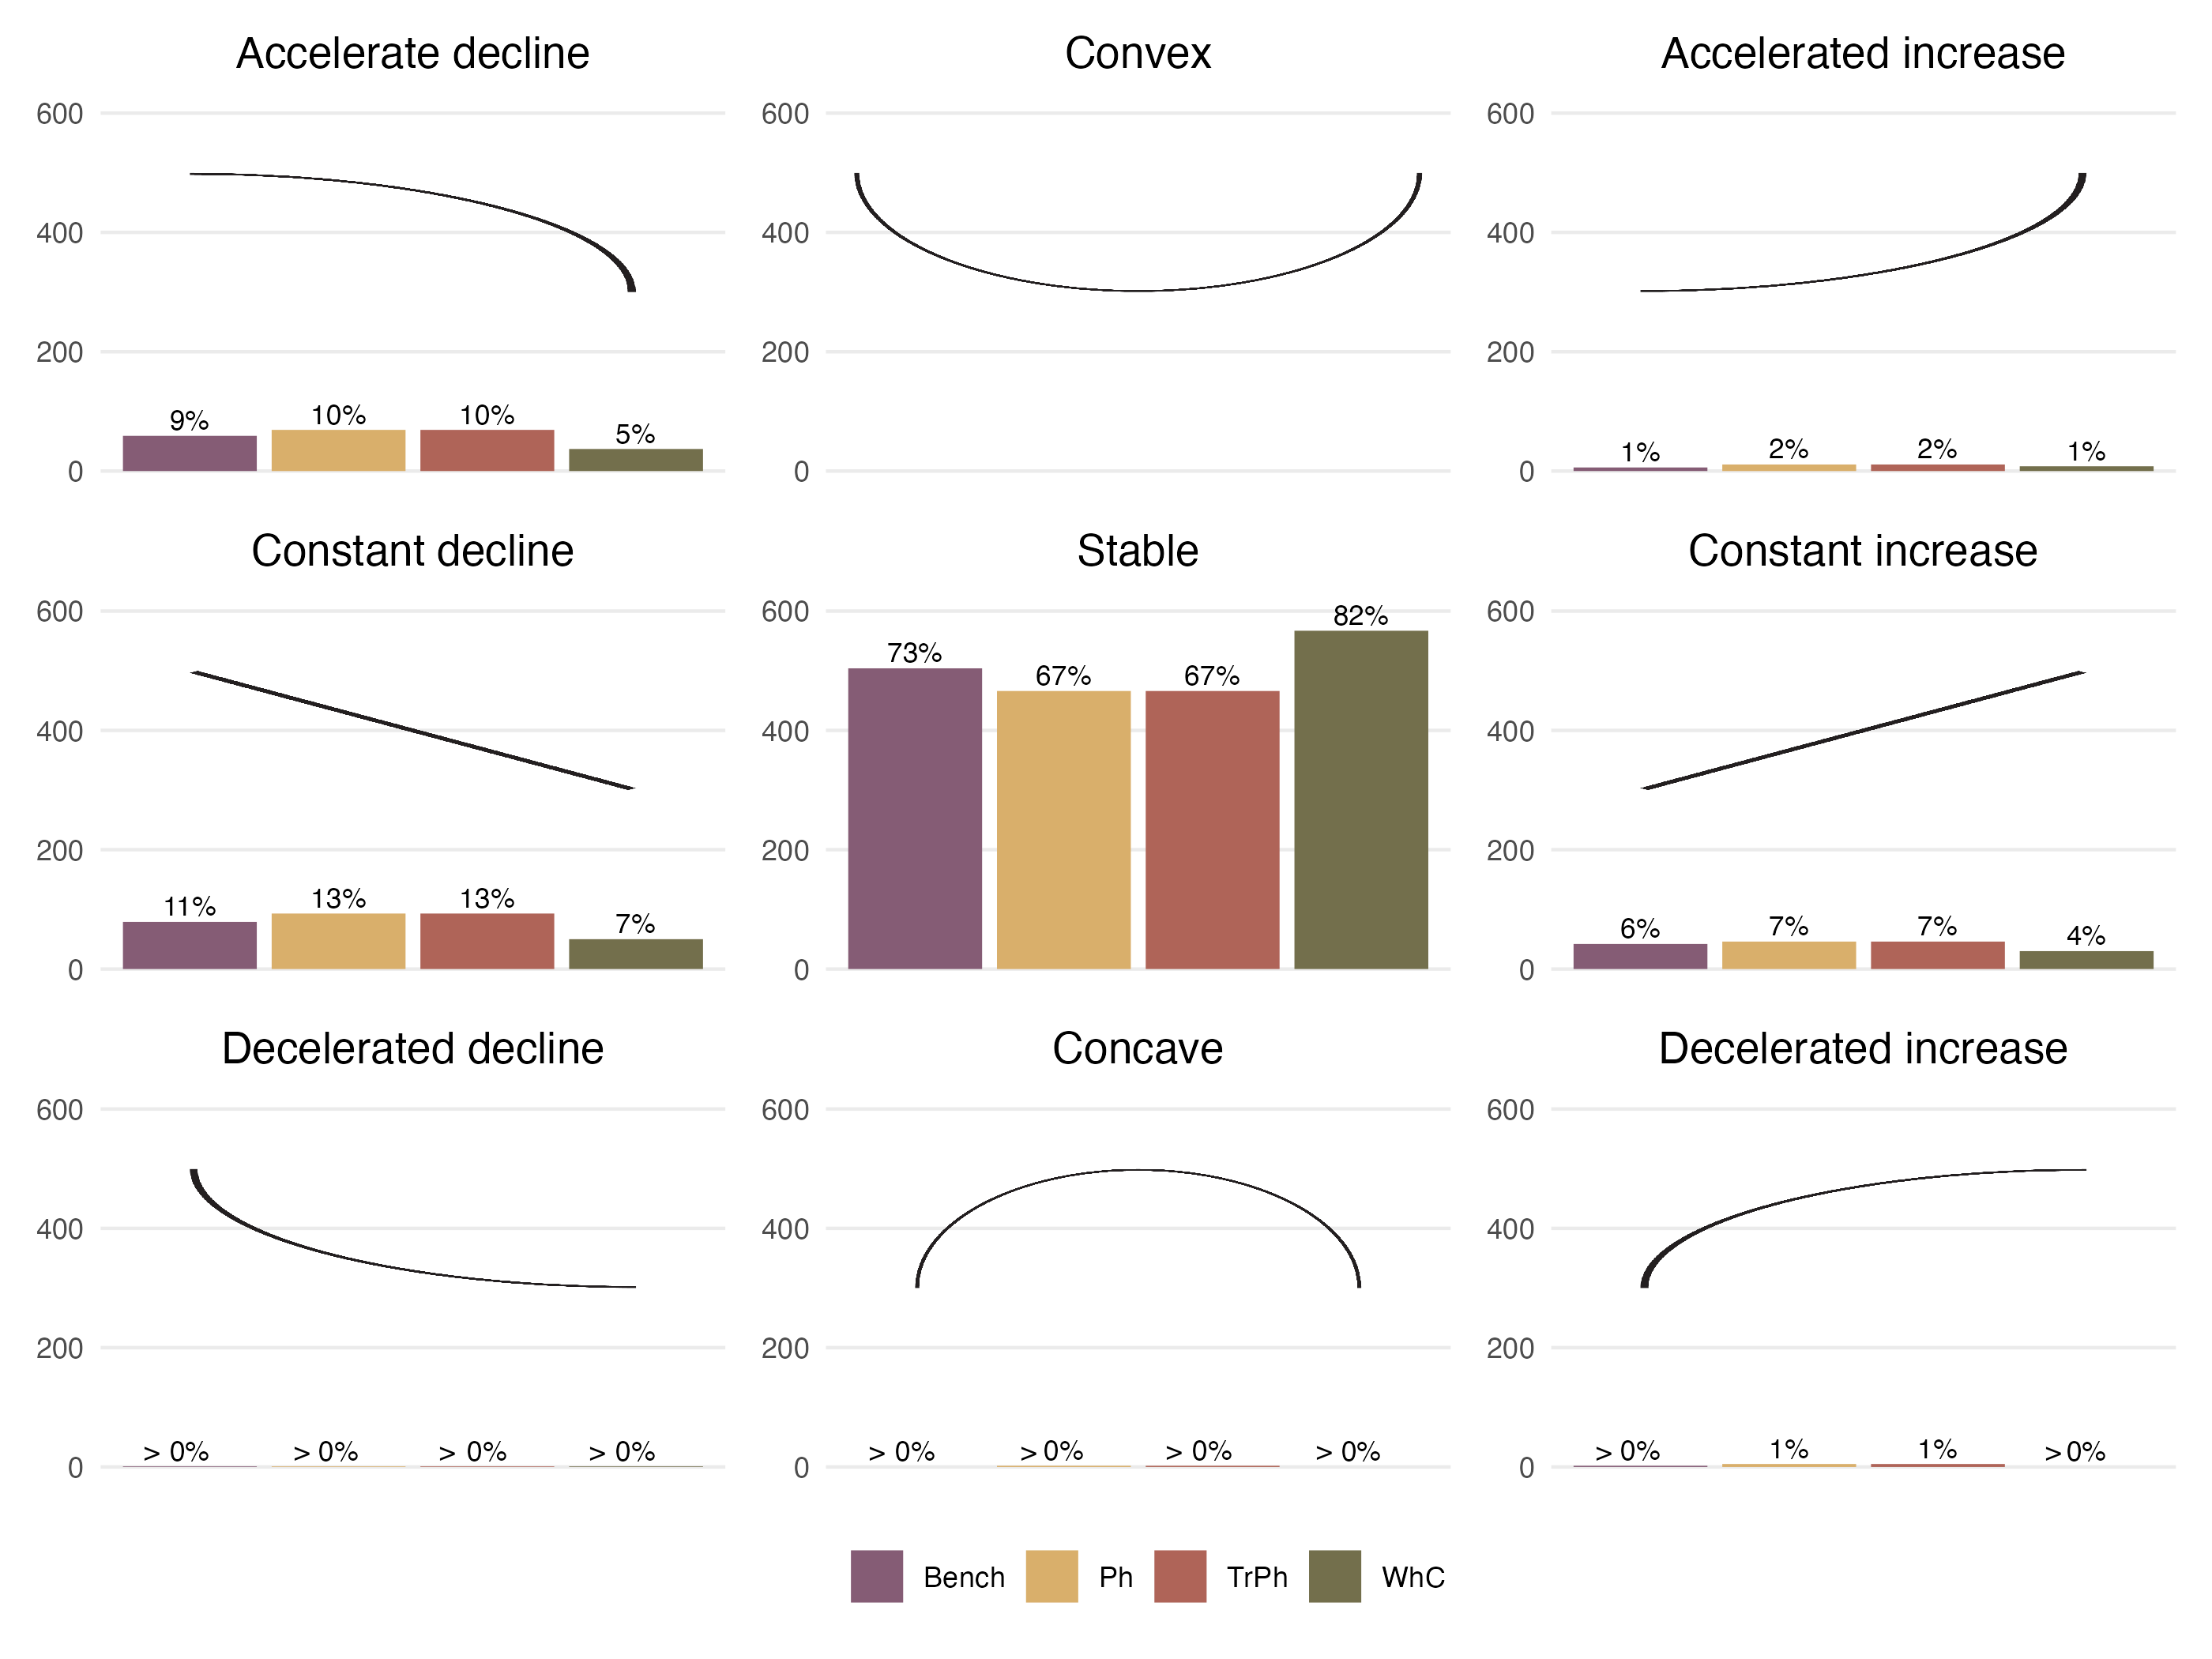
\includegraphics{03-Chapitre1/figures/supplementary/fig_supp25.png}
\caption{Same figure as Fig. 4 in the main text but for models fitted to
presence/absence data. Number (y-axis) and proportion (indicated above
individual bars, rounded to the nearest integer) of response curves
(i.e.~one for each species-predictor combination) according to the
nomenclature (nine shapes highlighted by the black curve in each panel)
defined by \textcite{Rigal_2020}. Results are presented for the
different structures: purple for the Benchmark (Bench), yellow for
phylogeny (Ph), red for traits \& phylogeny (TrPh), and green for whole
community (WhC) model.}\label{fig:chapt1supp25}
}
\end{figure}

\begin{figure}
\hypertarget{fig:chapt1supp27}{%
\centering
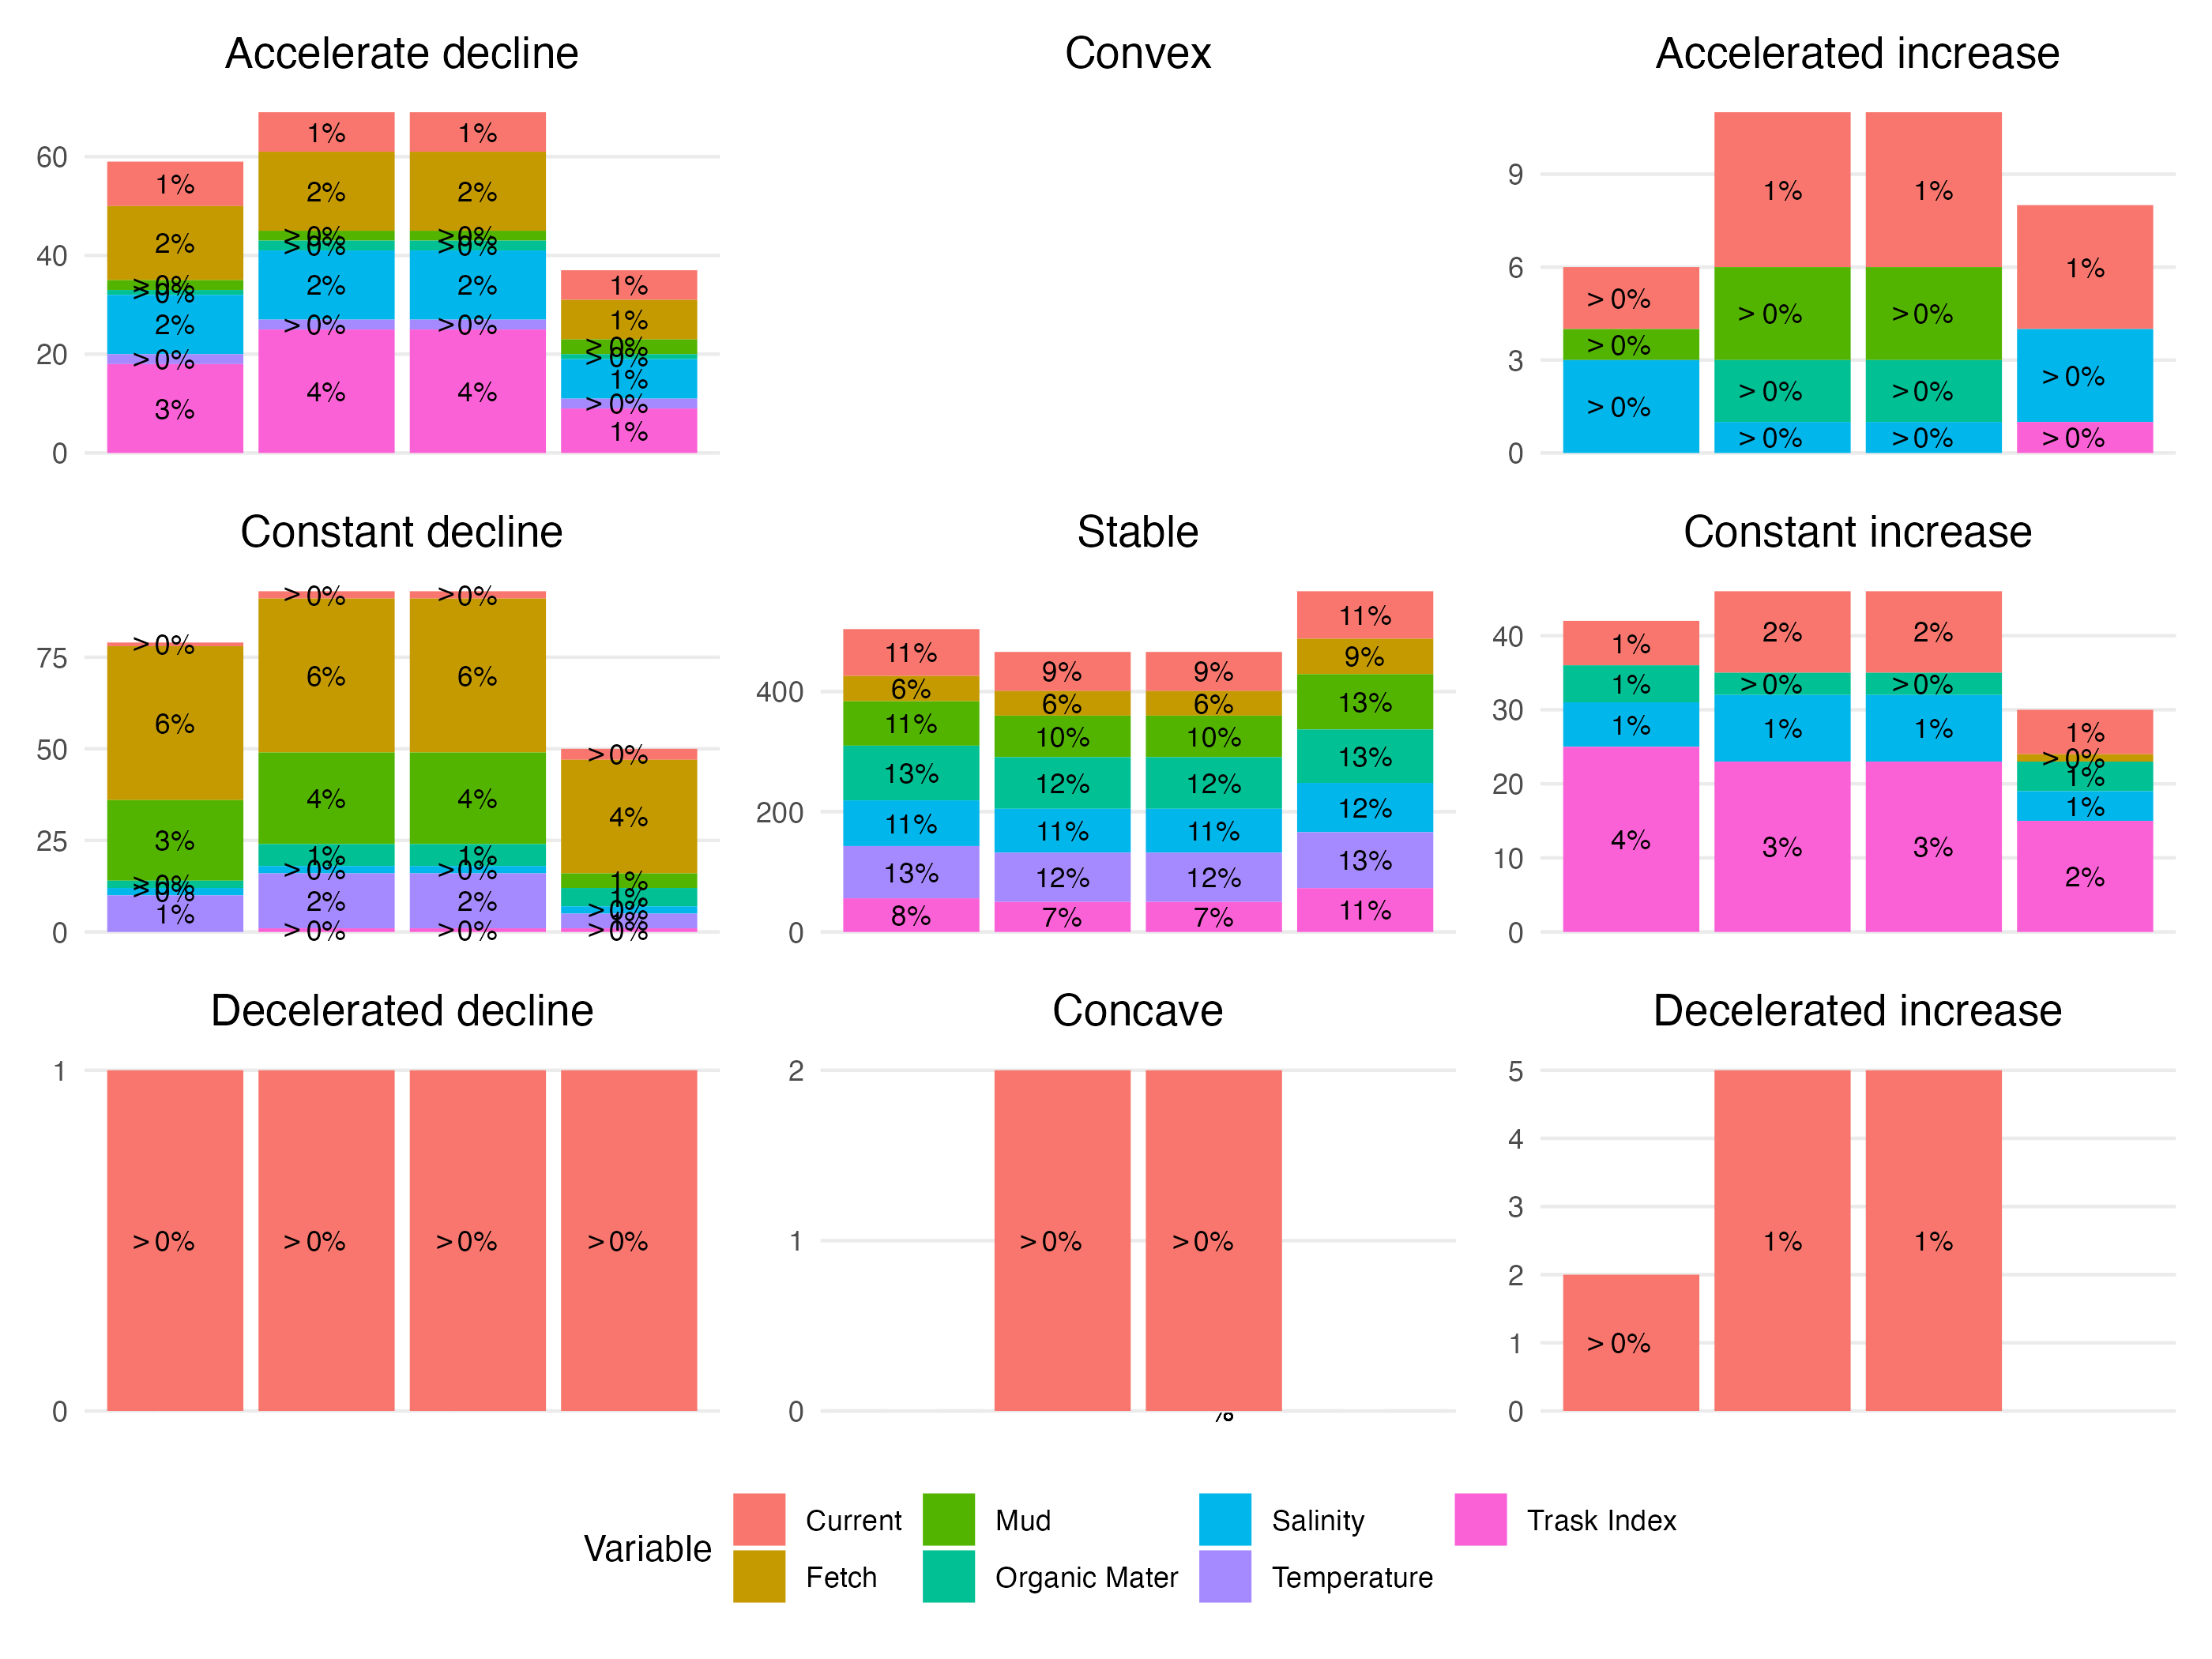
\includegraphics{03-Chapitre1/figures/supplementary/fig_supp27.png}
\caption{Same figure as Fig.~\ref{fig:chapt1supp26} but for models
fitted on presence/absence data. Number (y-axis) and proportion
(indicated above individual bars, rounded to the nearest integer) of
response curves (i.e.~one for each species-predictor combination)
according to the nomenclature (nine shapes highlighted by the black
curve in each panel) defined by \textcite{Rigal_2020} for different
presence/absence model structures. Each bar is coloured by the relative
contribution of each environmental covariate to this particular shape.
For illustrative purposes, note that the scale of variation on the
y-axis differs across panels.}\label{fig:chapt1supp27}
}
\end{figure}

\begin{figure}
\hypertarget{fig:chapt1supp28}{%
\centering
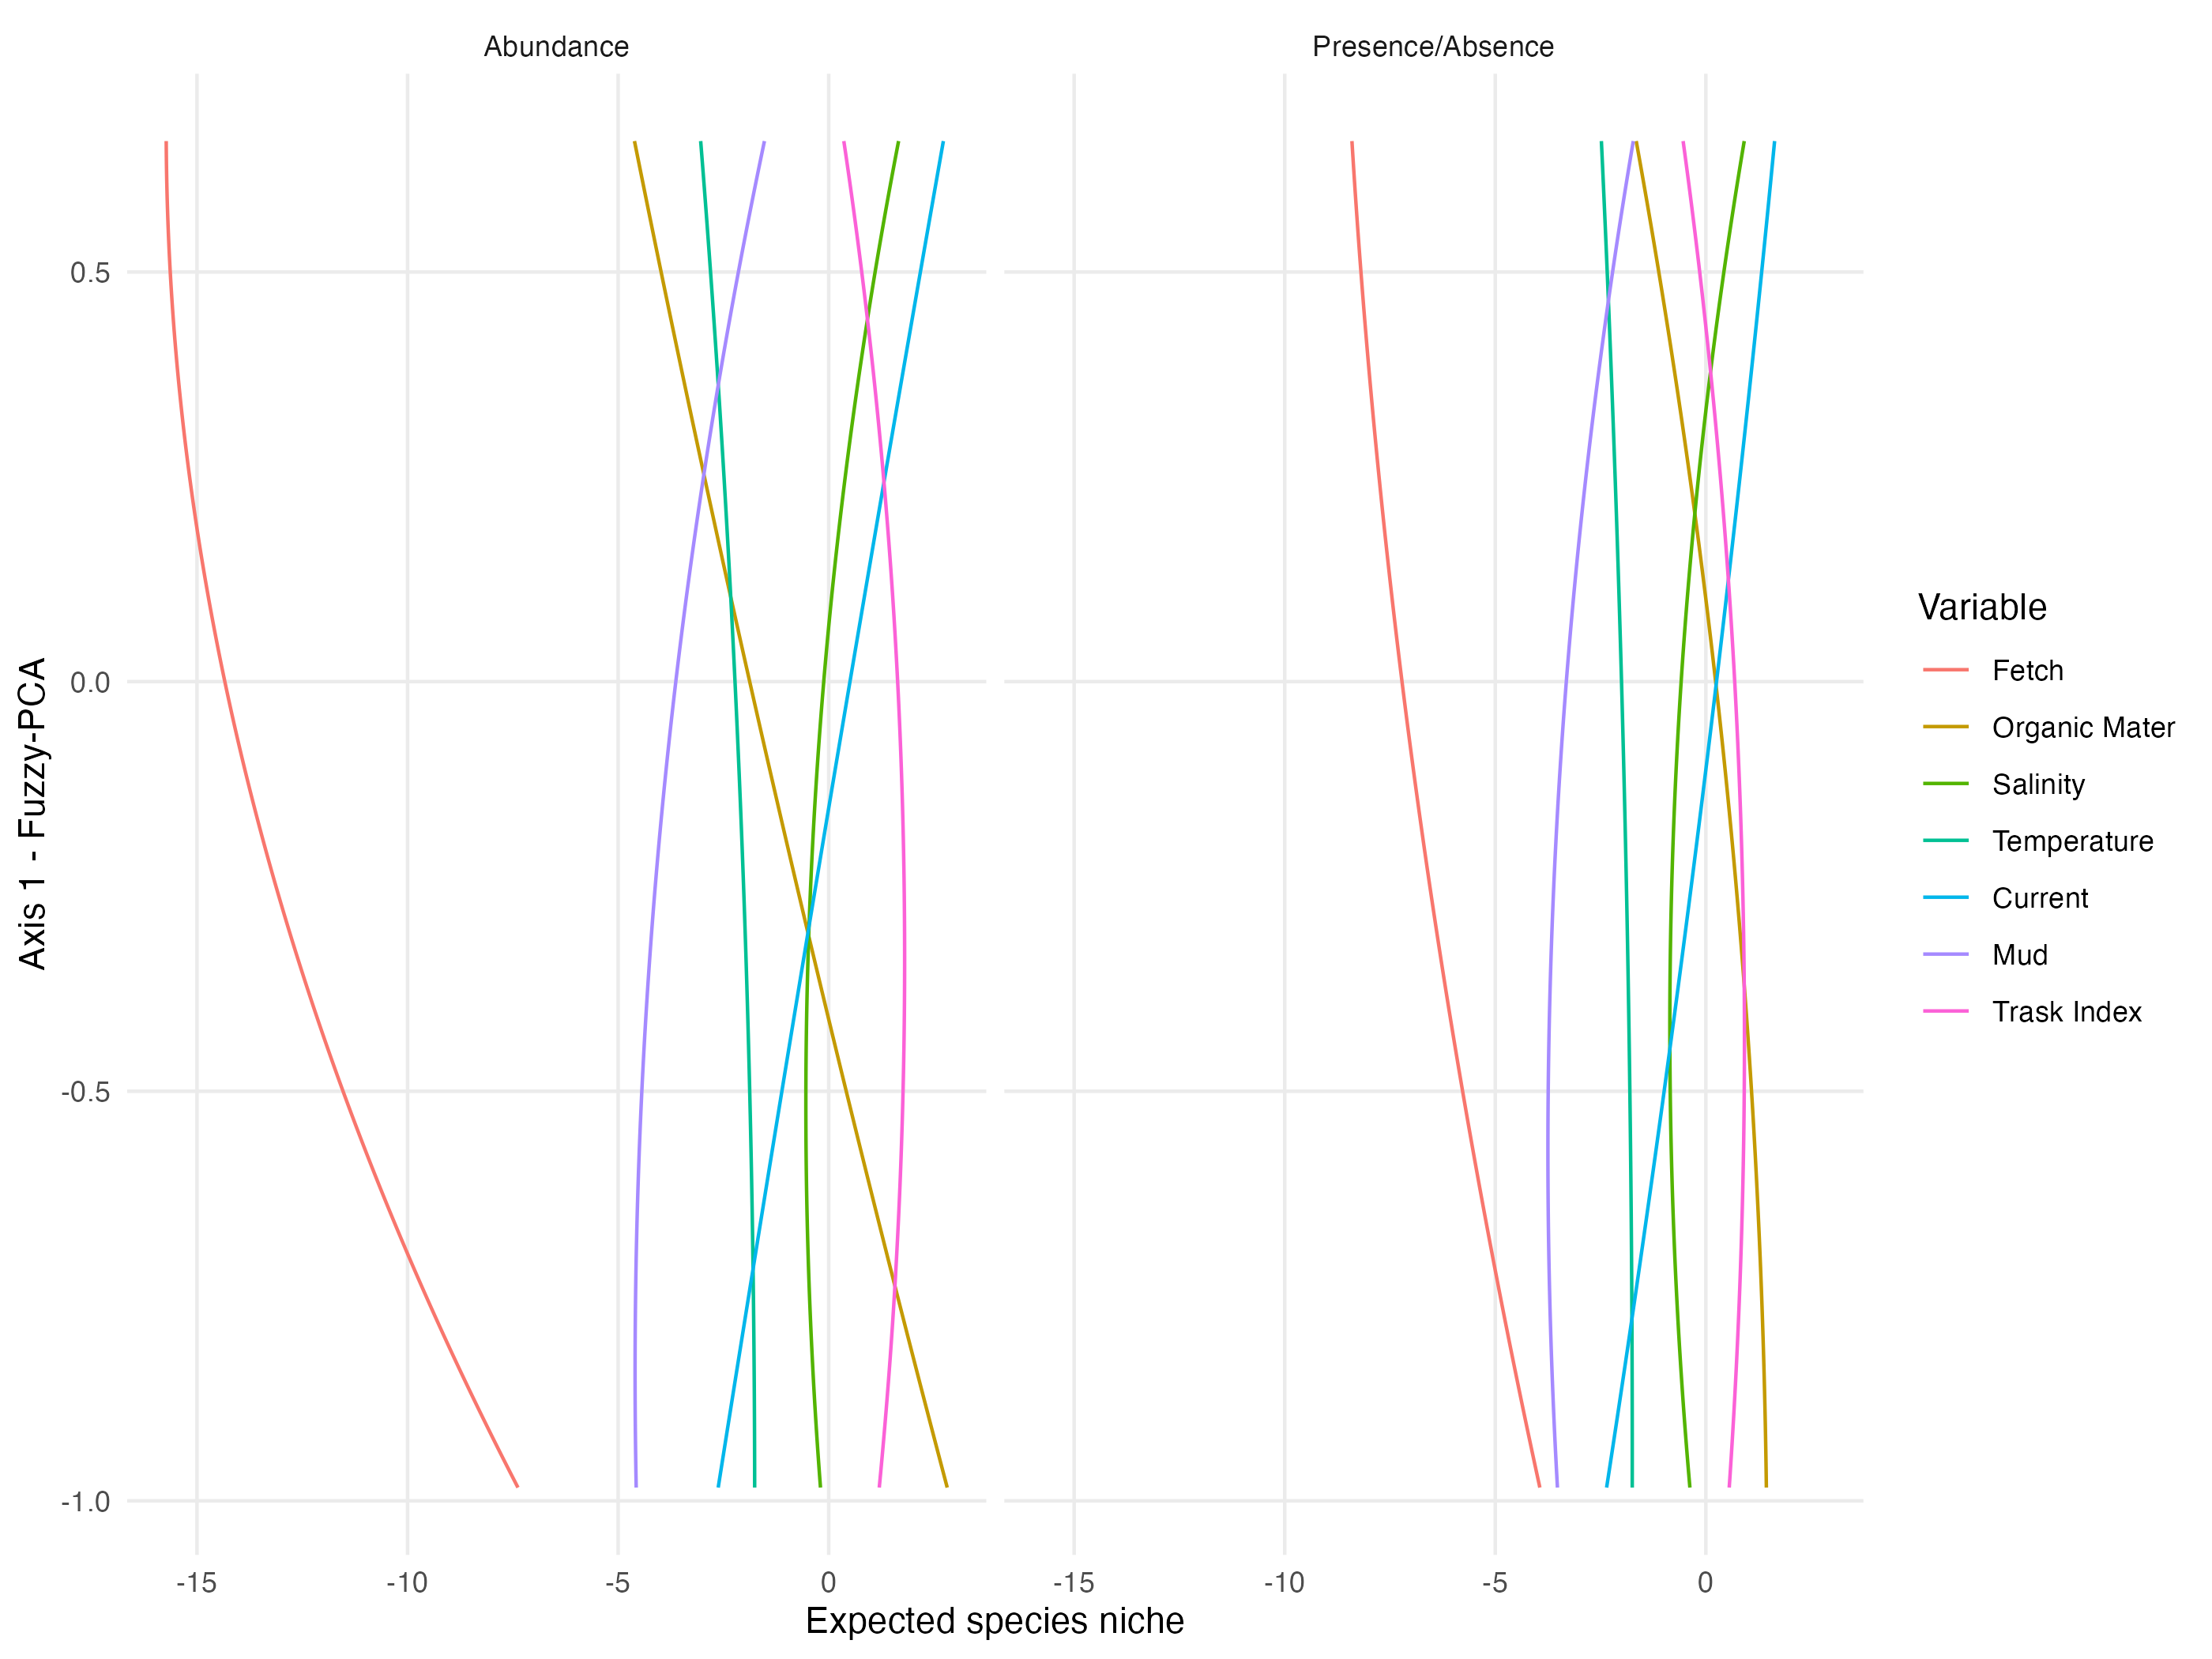
\includegraphics{03-Chapitre1/figures/supplementary/fig_supp28.png}
\caption{Relationship between species' position along the first axis of
the fuzzy PCA (sessile microphagous-mobile macrophagous gradient) and
the different environmental variables used in the models (fitted with
abundance data in the left panel, and with presence/absence data in the
right panel). Relationships are derived from the regression coefficients
estimated for the PhTr model (\(\gamma\) coefficients in HMSC;
\textcite{Ovaskainen_2020}).The lines are fitted quadratic regressions
representing the average response across the different species. As an
example of interpretation, the red lines in both graphs indicate that
sessile microphagous species are more negatively influenced (lower
abundance, low probability for presence) by fetch than macrophagous
mobile species.}\label{fig:chapt1supp28}
}
\end{figure}

\begin{figure}
\hypertarget{fig:chapt1supp30}{%
\centering
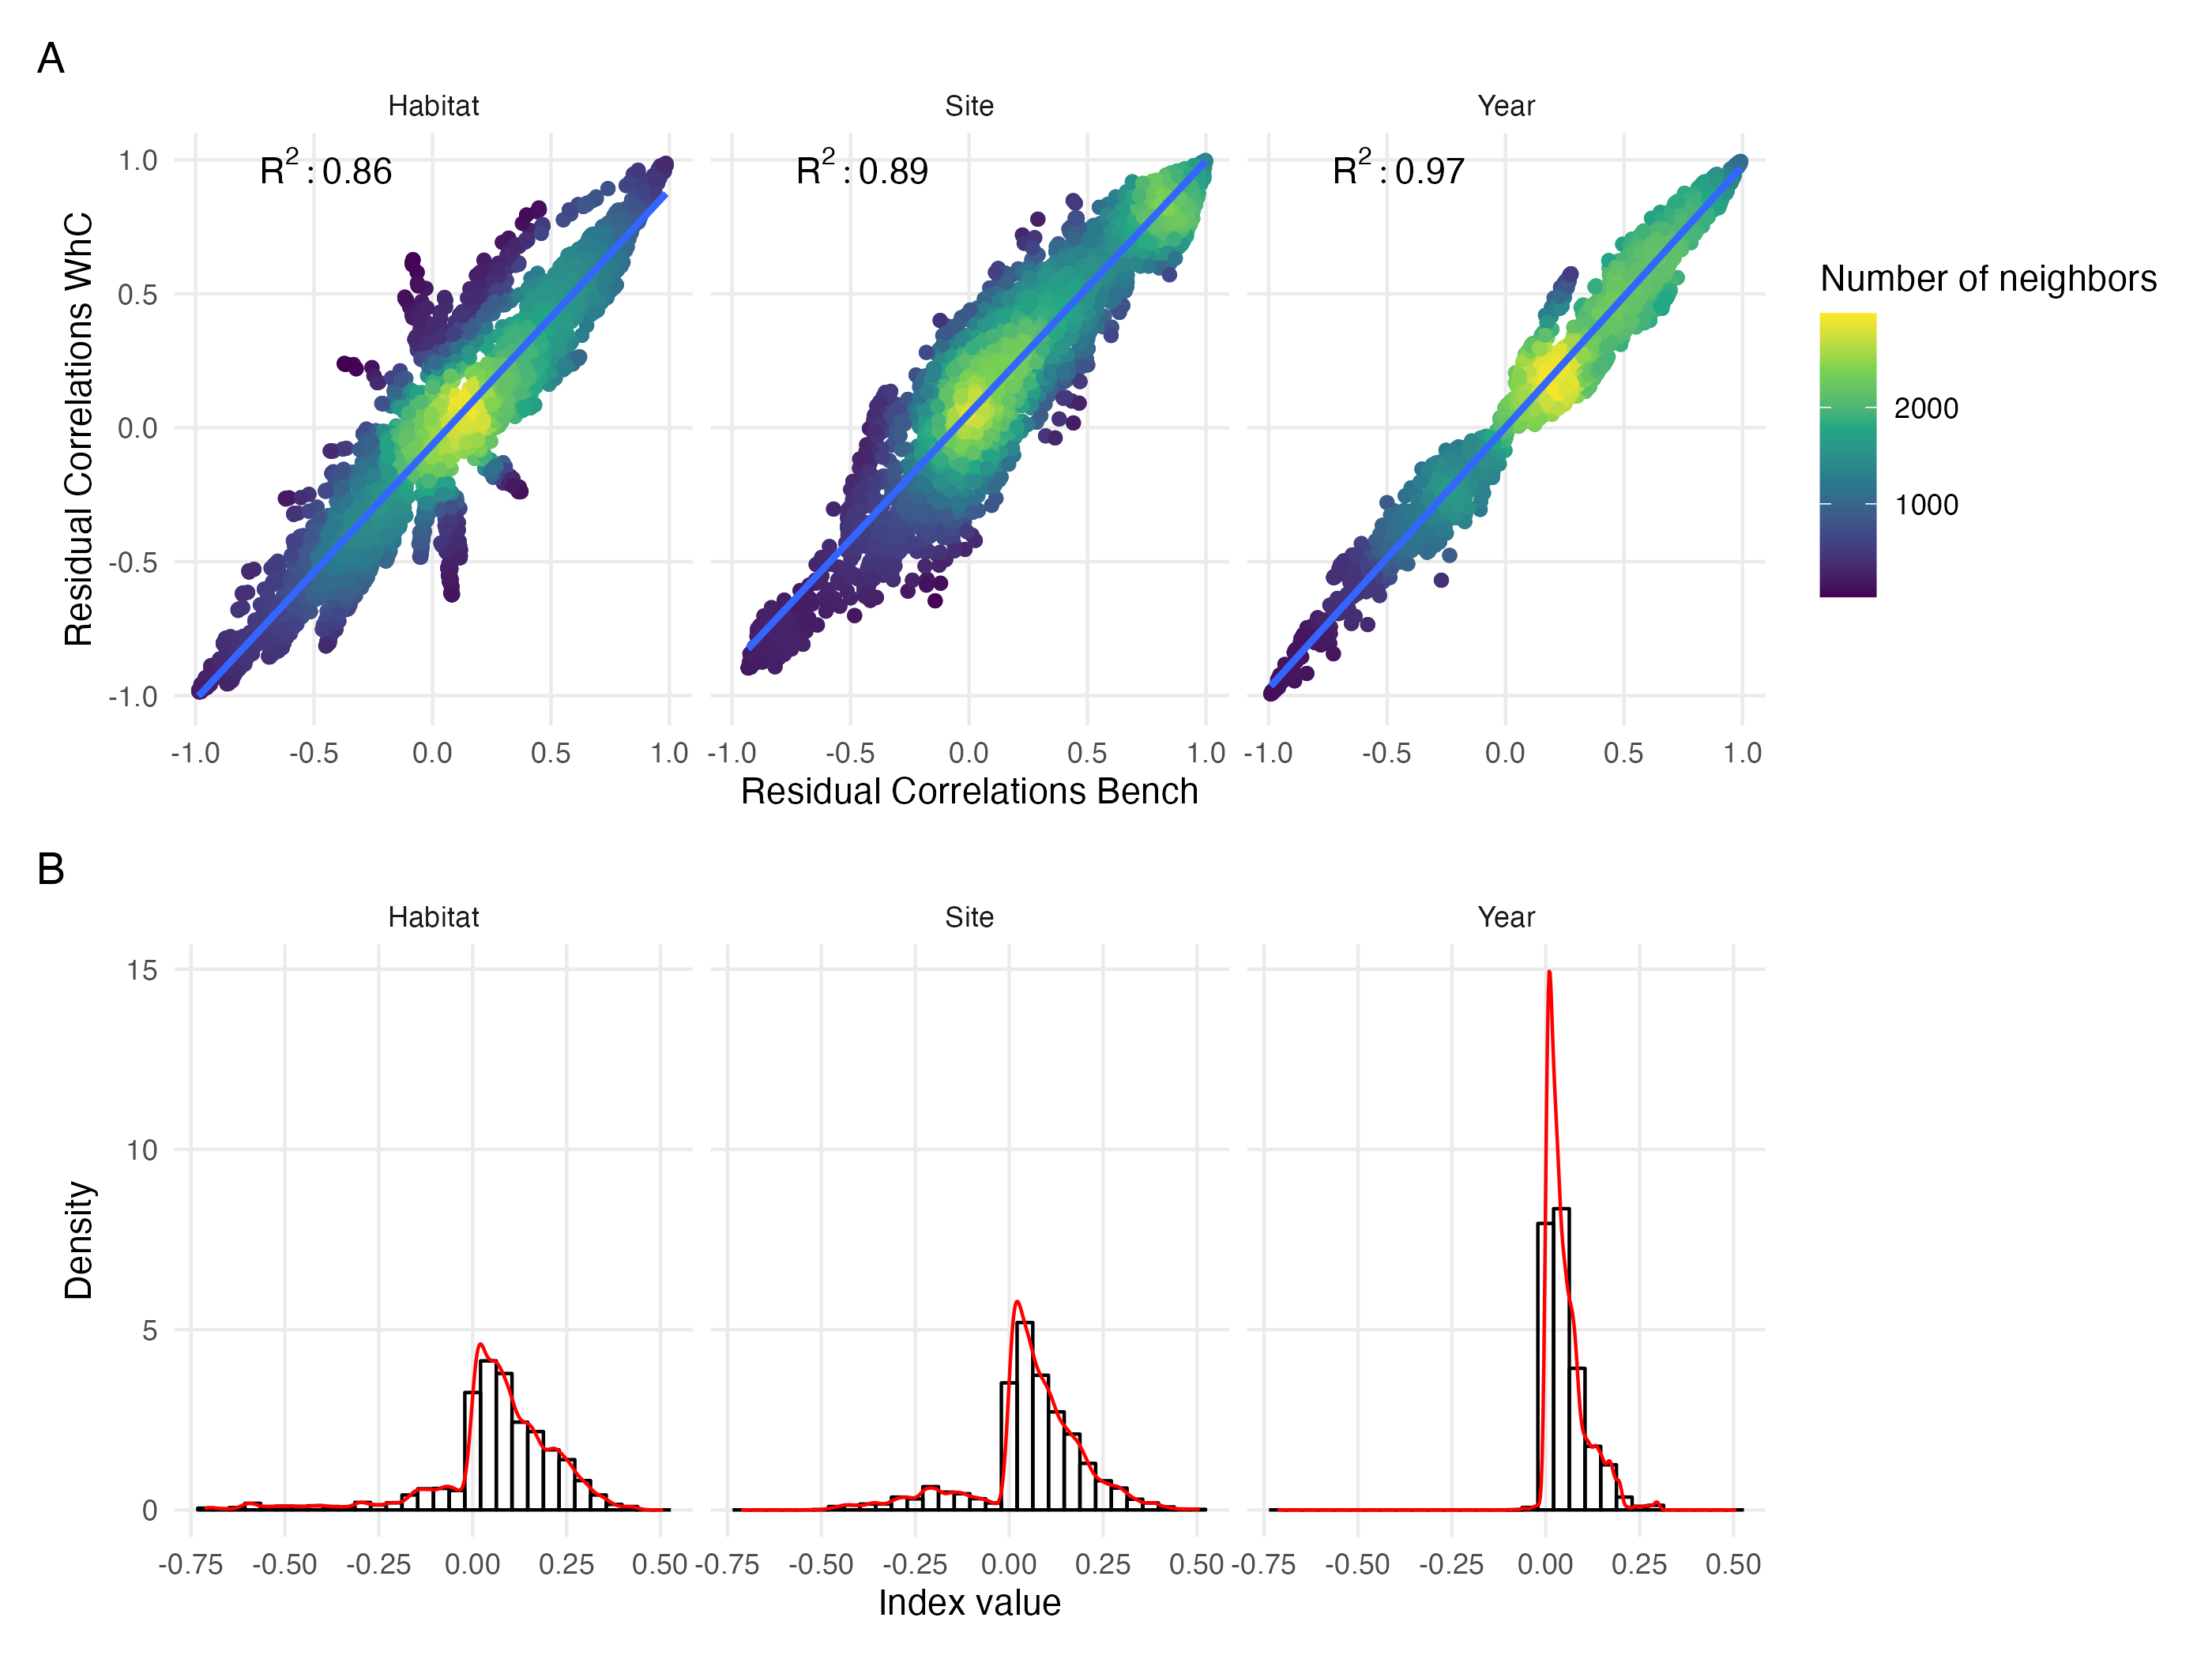
\includegraphics{03-Chapitre1/figures/supplementary/fig_supp29.png}
\caption{Same figure as Fig. 5 in the main text but for models fitted on
presence/absence data. (A) Comparison of residual correlations
associated with the three random effects estimated by the Whole
Community Model (y-axis) and the Benchmark model (x-axis). The colour
scale highlights the density of points in each scatter plot. (B)
Distribution of the index measuring change in sign (sign change left to
the zero line, no change to the right) and magnitude (higher departure
from the zero line indicate higher difference) between residual
correlations estimated by the whole community model and the benchmark
model for the three random effects (Habitat, Site,
Year).}\label{fig:chapt1supp30}
}
\end{figure}

% Restore all parameters as default

\let\sectionmark\oldsectionmark

\captionsetup[figure]{list=yes}
\captionsetup[table]{list=yes}

\renewcommand{\thefigure}{\arabic{figure}}
\renewcommand{\thetable}{\arabic{table}}   

% \setcounter{figure}{\value{savedfigure}}
% \setcounter{table}{\value{savedtable}}
\counterwithin{figure}{chapter}
\counterwithin{table}{chapter}

% End of subappendices environment
\AtEndEnvironment{subappendices}{%
}